
% !Mode:: "Tex:UTF-8"



\documentclass[10pt,a4paper]{article}\usepackage[]{graphicx}\usepackage[]{color}
%% maxwidth is the original width if it is less than linewidth
%% otherwise use linewidth (to make sure the graphics do not exceed the margin)
\makeatletter
\def\maxwidth{ %
  \ifdim\Gin@nat@width>\linewidth
    \linewidth
  \else
    \Gin@nat@width
  \fi
}
\makeatother

\definecolor{fgcolor}{rgb}{0.345, 0.345, 0.345}
\newcommand{\hlnum}[1]{\textcolor[rgb]{0.686,0.059,0.569}{#1}}%
\newcommand{\hlstr}[1]{\textcolor[rgb]{0.192,0.494,0.8}{#1}}%
\newcommand{\hlcom}[1]{\textcolor[rgb]{0.678,0.584,0.686}{\textit{#1}}}%
\newcommand{\hlopt}[1]{\textcolor[rgb]{0,0,0}{#1}}%
\newcommand{\hlstd}[1]{\textcolor[rgb]{0.345,0.345,0.345}{#1}}%
\newcommand{\hlkwa}[1]{\textcolor[rgb]{0.161,0.373,0.58}{\textbf{#1}}}%
\newcommand{\hlkwb}[1]{\textcolor[rgb]{0.69,0.353,0.396}{#1}}%
\newcommand{\hlkwc}[1]{\textcolor[rgb]{0.333,0.667,0.333}{#1}}%
\newcommand{\hlkwd}[1]{\textcolor[rgb]{0.737,0.353,0.396}{\textbf{#1}}}%
\let\hlipl\hlkwb

\usepackage{framed}
\makeatletter
\newenvironment{kframe}{%
 \def\at@end@of@kframe{}%
 \ifinner\ifhmode%
  \def\at@end@of@kframe{\end{minipage}}%
  \begin{minipage}{\columnwidth}%
 \fi\fi%
 \def\FrameCommand##1{\hskip\@totalleftmargin \hskip-\fboxsep
 \colorbox{shadecolor}{##1}\hskip-\fboxsep
     % There is no \\@totalrightmargin, so:
     \hskip-\linewidth \hskip-\@totalleftmargin \hskip\columnwidth}%
 \MakeFramed {\advance\hsize-\width
   \@totalleftmargin\z@ \linewidth\hsize
   \@setminipage}}%
 {\par\unskip\endMakeFramed%
 \at@end@of@kframe}
\makeatother

\definecolor{shadecolor}{rgb}{.97, .97, .97}
\definecolor{messagecolor}{rgb}{0, 0, 0}
\definecolor{warningcolor}{rgb}{1, 0, 1}
\definecolor{errorcolor}{rgb}{1, 0, 0}
\newenvironment{knitrout}{}{} % an empty environment to be redefined in TeX

\usepackage{alltt}
\usepackage{etoolbox}
\newtoggle{color}
%\togglefalse{color}
\toggletrue{color}

\usepackage{makeidx}
\newcommand{\idioma}{spanish}
\newcommand{\opcionesIdioma}{,es-nodecimaldot,es-tabla}
% !Mode:: "Tex:UTF-8"
%%%%%%%%%%%%%%%%%%%%%Carga de Packages
%%poner \newcommand{\idioma}{spanish} o \newcommand{\idioma}{english} en el documento
\usepackage{pdfsync}
\usepackage{srcltx}
\usepackage[\idioma\opcionesIdioma]{babel}
\usepackage[utf8x]{inputenc}
\usepackage[T1]{fontenc}
\usepackage{graphicx}
\graphicspath{{/users/fernando/figuras/}{./}{./figuras/}{/fernando/figuras/}{/fernando/figuras/jpg/}}
\usepackage{multicol}
\usepackage{epsfig}
%\usepackage{oberdiek}
\usepackage{listingsutf8}
\lstset{inputencoding=utf8/latin1}
%\lstset{extendedchars=true}
\lstset{ %
  language=R,                     % the language of the code
  basicstyle=\ttfamily\small,       % the size of the fonts that are used for the code
  numbers=left,                   % where to put the line-numbers
  numberstyle=\tiny\color{gray},  % the style that is used for the line-numbers
  stepnumber=1,                   % the step between two line-numbers. If it's 1, each line
                                  % will be numbered
  numbersep=5pt,                  % how far the line-numbers are from the code
  backgroundcolor=\color{white},  % choose the background color. You must add \usepackage{color}
  showspaces=false,               % show spaces adding particular underscores
  showstringspaces=false,         % underline spaces within strings
  showtabs=false,                 % show tabs within strings adding particular underscores
  frame=single,                   % adds a frame around the code
  rulecolor=\color{black},        % if not set, the frame-color may be changed on line-breaks within not-black text (e.g. commens (green here))
  tabsize=2,                      % sets default tabsize to 2 spaces
  %captionpos=,                   % sets the caption-position to bottom
  breaklines=true,                % sets automatic line breaking
  breakatwhitespace=false,        % sets if automatic breaks should only happen at whitespace
  %title=\lstname,                 % show the filename of files included with \lstinputlisting;
                                  % also try caption instead of title
  keywordstyle=\color{black},      % keyword style
  commentstyle=\color{Brown},   % comment style
  stringstyle=\color{black},      % string literal style
  escapeinside={\%*}{*)},         % if you want to add a comment within your code
  morekeywords={*,...},            % if you want to add more keywords to the set
  lineskip={-2.5pt} % single line spacing
}
%\usepackage{algorithm}
\usepackage{amsmath}
\usepackage{amsfonts}
\usepackage{amssymb}
\usepackage{amsthm}
\usepackage{fancybox}
\usepackage{fancyvrb}
\usepackage{rotating}
\usepackage{keystroke}
\usepackage{array}
\input{xy}
\xyoption{all}
%\usepackage[dvipsnames,usenames]{color}
\usepackage[usenames,dvipsnames,svgnames,table]{xcolor}
\usepackage{colortbl}
\usepackage{comment}
\excludecomment{spanish}
\excludecomment{english}
\includecomment{\idioma}

%\usepackage{noweb}
%\usepackage{clrscode}
\usepackage{eurosym}
\usepackage{wasysym}
\usepackage{multirow}
%\usepackage{margins}
\usepackage{lscape}
\usepackage{longtable}
\usepackage[normalem]{ulem}
\usepackage{xr-hyper}

%%NUEVO
\newcolumntype{C}{{\centering\arraybackslash}m{20mm}}
\newcommand{\centercell}[1]{\multicolumn{1}{c}{#1}}
\newcommand{\colHead}[1]{\centercell{\bfseries#1}}

\excludecomment{ocultar}


% Matriz (par‚ntesis)
\def\matr#1#2{\left(\begin{array}{#1}#2\end{array}\right)}
% Determinante (barras)
\def\deter#1#2{\left|\begin{array}{#1}#2\end{array}\right|}
% Sistema de ecuaciones. (llave a la izda.)
\def\seq#1#2{\left\{\begin{array}{#1}#2\end{array}\right.}
% Ecuaci\'on de varias lineas (sin llave a la izda.)
\def\evl#1#2{\begin{array}{#1}#2\end{array}}

%%%%%%%%%%%%%%%%%%%%%%%%%%%%%%%%%%%%%%%%%%%%%%
%%%%%%%%%%%%%%%%%%%%%%%%%%%%%%%%%%%%%%%%%%%%%%
%%%%%%%%%%%%%%%%% M\'{a}rgenes %%%%%%%%%%%%%%%%
%
%
%\parindent=0mm
%
%\textwidth=160mm
%\textheight=220mm
%\hoffset=-20mm
%\voffset=-15mm
%\parskip=0mm
\marginparsep=3mm
\marginparwidth=25mm
%
%%%%%%%%%%%%%%%%%%%%%%%%%%%% Contadores para listas de problemas
%\newcommand{\adc}{\addtocounter{enumi}{1}}
\newcommand{\adc}{\stepcounter{enumi}}
\newcommand{\adci}{\stepcounter{enumii}}
\newcommand{\xadc}{\addtocounter{xcounter}{1}}
\newcommand{\be}{\begin{enumerate}}
\newcommand{\ee}{\end{enumerate}}
\newcommand{\bi}{\begin{itemize}}
\newcommand{\ei}{\end{itemize}}
\newcounter{xcounter}


\newcommand{\nin}{{\noindent}}

%\newcounter{prob}{}
%\def\pr{\addtocounter{prob}{1}(\theprob)\ }
%\def\pr2{\addtocounter{prob}{2}(\theprob)\ }

%%%%%%%%%%%%%%%%%%%%%%%%%%%Fin de demostraciones, ejemplos, etc.
\newcommand{\fin}{$\square$}
%%%%%%%%%%%%%%%%%%%%%%%%%%Notaci\'{o}n matem\'{a}ticas generales
%\newcommand{\suc}[1]{\{#1_n\}}
%\newcommand{\sucn}[1]{\{#1_n\}_{n\in\mathbb{N}}}
%\newcommand{\ser}[1]{\sum #1_n}
%\newcommand{\sern}[1]{\sum_{n\geq 1} #1_n}
%\newcommand{\limn}{\lim_{n\rightarrow\infty}}
%\newcommand{\limnd}{\displaystyle\lim_{n\rightarrow\infty}}
%\newcommand{\mf}[1]{\mathbf{#1}}
%\newcommand{\mb}[1]{\mathbb{#1}}
%\newcommand{\D}[1]{\Dv_{\mf{#1}}}
%\newcommand{\bsigma}{\pmb{\sigma}}
%\newcommand{\bPhi}{\pmb{\Phi}}
%\newcommand{\vol}{\operatorname{vol}}
%\newcommand{\ldbr}{[\hspace{-1.5pt}[}
%\newcommand{\rdbr}{]\hspace{-1.5pt}]}
%\newcommand{\fpws}[2]{{#1}\ldbr{#2}\rdbr}
%\newcommand{\leftPui}{<\hspace{-3pt}<}
%\newcommand{\rightPui}{\hspace{-3pt}}
%\newcommand{\Pui}[2]{{#1}\hspace{-6pt}\leftPui{#2}\rightPui}
%\newcommand{\pdd}[2]{\dfrac{\partial{#1}}{\partial{#2}}}
%%%%%%%%%%Conjuntos de n\'{u}meros
\newcommand{\N}{\mathbb{N}} %conjunto de n\'{u}meros naturales
\newcommand{\Z}{\mathbb{Z}} %conjunto de n\'{u}meros enteros
\newcommand{\R}{\mathbb{R}} %conjunto de n\'{u}meros reales
\newcommand{\C}{\mathbb{C}} %conjunto de n\'{u}meros complejos
\newcommand{\Q}{\mathbb{Q}} %conjunto de n\'{u}meros racionales
\newcommand{\EP}{\mathbb{P}} %espacios proyectivos
\newcommand{\K}{\mathbb{K}} %cuerpo gen\'{e}rico
\newcommand{\A}{\mathbb{A}} %espacios afines

%%%%%%%%%%Estadistica
\newcommand{\MEAN}{\mathrm{E}}
\newcommand{\Var}{\mathrm{Var}}
\newcommand{\Cov}{\mathrm{Cov}}


%%%%%%%%%%Funciones
\def\arcsen{\operatorname{arcsen}}
\def\arctg{\operatorname{arctg}}
\def\argCosh{\operatorname{argCosh}}
\def\argSenh{\operatorname{argSenh}}
\def\argTgh{\operatorname{argTgh}}
\def\cosec{\operatorname{cosec}}
\def\Cosh{\operatorname{Cosh}}
\def\cotg{\operatorname{cotg}}
\def\Dv{\operatorname{D}}
\def\discrim{\operatorname{discrim}}
\def\dive{\operatorname{div}}
\def\dom{\operatorname{dom}}
\def\Ext{\operatorname{Ext}}
\def\Fr{\operatorname{Fr}}
\def\dder#1#2{\dfrac{d #1}{d #2} } %derivada en estilo display
\def\gr{\operatorname{gr}}
\def\grad{\operatorname{grad}}
\def\Imag{\operatorname{Im}}
\def\mcm{\operatorname{mcm}}
\def\rang{\operatorname{rang}}
\def\rot{\operatorname{rot}}
\def\sen{\operatorname{sen}}
\def\Senh{\operatorname{Senh}}
\def\sgn{\operatorname{sgn}}
\def\sig{\operatorname{sig}}
\def\tg{\operatorname{tg}}
\def\Tgh{\operatorname{Tgh}}
\def\E{\operatorname{E}}
\def\VAR{\operatorname{VAR}}
\newcommand{\margWeb}[2]{\noindent{#2}\marginpar[\hspace{-18mm}\link{#1}{WEB}]{\hspace*{-18mm}\link{#1}{WEB}}}

%%%%%%%%%%%%%%%%%%%%%%\'{A}lgebra conmutativa.
\def\multideg{\operatorname{multideg}} %multidegree of a polynomial
\def\LT{\operatorname{lt}} %leading term of a polynomial
\def\LC{\operatorname{lc}} %leading coefficient of a polynomial
\def\LM{\operatorname{lm}} %leading monomial of a polynomial
\def\Mexp{\mathbb{Z}^n_{\geq 0}} %set of multiexponents of monomials
\def\set#1{\left\{{#1}\right\}}
\newcommand{\vlist}[2]{\mbox{${#1}_{1},\ldots,{#1}_{#2}$}}
\def\deg{\operatorname{deg}} %grado de un polinomio
\def\cp{\operatorname{cp}} %coeficiente principal de un polinomio
\def\CP{\operatorname{cp}} %coeficiente principal de un polinomio
\def\set#1{\left\{{#1}\right\}} %llaves de conjunto
\newcommand{\V}{{\bf V}} %variedad de un conjunto de polinomios
\newcommand{\I}{{\bf I}} %ideal de un conjunto
\newcommand{\MCD}{\operatorname{mcd}} %m\'{a}ximo com\'{u}n divisor
\newcommand{\MCM}{\operatorname{mcm}} %m\'{\i}nimo com\'{u}n m\'{u}ltiplo
\newcommand{\LCM}{\operatorname{lcm}} %least common multiple
\newcommand{\GCD}{\operatorname{gcd}} %greatest common divisor
\newcommand{\Ker}{\operatorname{Ker}} %N\'{u}cleo
\newcommand{\IM}{\operatorname{IM}} %Imagen
\newcommand{\Rad}{\operatorname{Rad}} %radical de un ideal
\newcommand{\Jac}{\operatorname{Jac}} %radical de Jacobson de un anillo
\newcommand{\Ann}{\operatorname{Ann}} %anulador de un ideal
\newcommand{\Res}{\operatorname{Res}} %resultante de polinomios
\newcommand{\Mult}{\operatorname{mult}} %multiplicidad
\newcommand{\Gen}{\operatorname{Gen}} %g\'{e}nero
\newcommand{\Card}{\operatorname{Card}} %cardinal
\newcommand{\ord}{\operatorname{ord}} %orden
\newcommand{\prim}{\operatorname{prim}} %parte primitiva
\newcommand{\NP}{\operatorname{NP}} %NP idea
\newcommand{\cont}{\operatorname{cont}} %parte primitva
\newcommand{\pp}{\operatorname{pp}} %parte primitva
\newcommand{\PP}{\mathop{\mathrm{PP}}\nolimits}
\newcommand{\Int}{\operatorname{Int}}
\newcommand{\Ind}{\operatorname{index}}
\newcommand{\Lcoeff}{\operatorname{lc}} %leading coefficient of a polynomial
\newcommand{\Sqf}{\operatorname{Sqf}} %square free part of a polynomial

\def\pd#1#2{\frac{\partial #1}{\partial #2}} %derivada parcial
\def\mult{\text{mult}} %multiplicity
\def\Sing{\text{Sing}} %multiplicity
\def\Cl#1{\overline{#1}} %cierre topol\'{o}gico
\def\fobox#1{\begin{center}\fbox{$\displaystyle #1 $}\end{center}}

%\newcommand{\Ext}{\operatorname{Ext}}

%%%%%%%%%%%%%%%%%%%%%%%%
%% unpunto mayor que cdot, pero menor que bullet
\newcommand{\sbt}{\,\begin{picture}(-1,1)(-1,-3)\circle*{3}\end{picture}\ }

%%%%%%%%%%%%%%%%%%%%%%%%S\'{\i}mbolos rodeados de un c\'{\i}rculo
\def\circled#1{\xymatrix{*+[o][F]{#1}}}

%%%%%%%%%%%%%%%%%%%Geometr\'{\i}a
\newcommand{\CH}{{\cal CH}} %%cierre convexo

%%%%%%%%%%%%%%%%%%%%Tipos de letra especiales
%%Caligr\'{a}ficas
\newcommand{\cA}{{\cal A}}
\newcommand{\cB}{{\cal B}}
\newcommand{\cC}{{\cal C}}
\newcommand{\cD}{{\cal D}}
\newcommand{\cE}{{\cal E}}
\newcommand{\cF}{{\cal F}}
\newcommand{\cG}{{\cal G}}
\newcommand{\cH}{{\cal H}}
\newcommand{\cI}{{\cal I}}
\newcommand{\cJ}{{\cal J}}
\newcommand{\cK}{{\cal K}}
\newcommand{\cL}{{\cal L}}
\newcommand{\cM}{{\cal M}}
\newcommand{\cN}{{\cal N}}
\newcommand{\cO}{{\cal O}}
\newcommand{\cP}{{\cal P}}
\newcommand{\cQ}{{\cal Q}}
\newcommand{\cR}{{\cal R}}
\newcommand{\cS}{{\cal S}}
\newcommand{\cT}{{\cal T}}
\newcommand{\cU}{{\cal U}}
\newcommand{\cV}{{\cal V}}
\newcommand{\cW}{{\cal W}}
\newcommand{\cX}{{\cal X}}
\newcommand{\cY}{{\cal Y}}
\newcommand{\cZ}{{\cal Z}}

%%%%%%%%%%%%%%%%%%%%%%%%%%Notaci\'{o}n matem\'{a}ticas generales
\newcommand{\sucn}[1]{\{#1_n\}_{n\in\mathbb{N}}}
\newcommand{\ser}[1]{\sum #1_n}
\newcommand{\sern}[1]{\sum_{n\geq 1} #1_n}
\newcommand{\limn}{\lim_{n\rightarrow\infty}}
\newcommand{\mf}[1]{\mathbf{#1}}
\newcommand{\mb}[1]{\mathbb{#1}}
\newcommand{\D}[1]{\Dv_{\mf{#1}}}
\newcommand{\bsigma}{\pmb{\sigma}}
\newcommand{\bPhi}{\pmb{\Phi}}
\newcommand{\vol}{\operatorname{vol}}
\newcommand{\ldbr}{[\hspace{-1.5pt}[}
\newcommand{\rdbr}{]\hspace{-1.5pt}]}
\newcommand{\fpws}[2]{{#1}\ldbr{#2}\rdbr}
\newcommand{\leftPui}{<\hspace{-3pt}<}
\newcommand{\rightPui}{\hspace{-3pt}}
\newcommand{\Pui}[2]{{#1}\hspace{-6pt}\leftPui{#2}\rightPui}
\newcommand{\pdd}[2]{\dfrac{\partial{#1}}{\partial{#2}}}


%\newcounter{contEnlace}

%\newcommand{\pendiente}{\textcolor{purple}{PENDIENTE: }}
%\newcommand{\link}[2]{\textcolor{blue}{{\href{#1}{#2}}}}


\iftoggle{color}{%
  % color version
  \newcommand{\pendiente}{\textcolor{red}{PENDIENTE: }}
  \newcommand{\link}[2]{\textcolor{blue}{{\href{#1}{#2}}}}
  \newcommand{\fichero}[2]{\textattachfile{#1}{\textcolor{blue}{#2}}}
  \newcommand{\otrofichero}[2]{\textattachfile{./datos/#1}{\textcolor{blue}{#2}}}
}{%
  % b/w version
  \newcommand{\pendiente}{\textcolor{black}{\underline{PENDIENTE:} }}
  \newcommand{\link}[2]{\textcolor{black}{{\href{#1}{\underline{#2}}}}}
  \newcommand{\fichero}[2]{\textattachfile{#1}{\textcolor{black}{\underline{#2}}}}
  \newcommand{\otrofichero}[2]{\textattachfile{./datos/#1}{\textcolor{black}{\underline{#2}}}}
}



%{\textcolor{blue}{{\href{#1}{#2}}}}

%%%%%%%%%%%%%%%%%%COLORES

\DefineNamedColor{named}{Brown}{cmyk}{0,0.81,1,0.60}
\definecolor{Gris050}{gray}{0.50}
\definecolor{Gris025}{gray}{0.75}
\definecolor{Gris010}{gray}{0.90}


%%%%%%%%%%%%%%%%%%%%%Package Algorithms
%\begin{spanish}
%\renewcommand{\algorithmicrequire}{{precondici\'{o}n:}}
%\renewcommand{\algorithmicensure}{{postcondici\'{o}n:}}
%\renewcommand{\algorithmicend}{{fin}}
%\renewcommand{\algorithmicif}{{si}}
% \renewcommand{\algorithmicthen}{{entonces}}
% \renewcommand{\algorithmicelse}{{si no}}
% \renewcommand{\algorithmicelsif}{\algorithmicelse\ \algorithmicif}
% \renewcommand{\algorithmicendif}{\algorithmicend\ \algorithmicif}
% \renewcommand{\algorithmicfor}{{para}}
% \renewcommand{\algorithmicforall}{{para todo}}
% \renewcommand{\algorithmicdo}{{hacer}}
% \renewcommand{\algorithmicendfor}{\algorithmicend\ \algorithmicfor}
% \renewcommand{\algorithmicwhile}{{mientras}}
% \renewcommand{\algorithmicendwhile}{\algorithmicend\ \algorithmicwhile}
% \renewcommand{\algorithmicrepeat}{{repetir}}
% \renewcommand{\algorithmicuntil}{{hasta}}
% \end{spanish}

%%%%%%%%%%%%%%%%%%%%%%%%%%%%%%%%%%Package Amsthm
\begin{spanish}
%\theoremstyle{definition}% default
\theoremstyle{plain}
\newtheorem{thm}{Teorema}[section]
\newtheorem{teo}{Teorema}[section]
\newtheorem{teorema}{Teorema}[section]
\newtheorem{lem}[thm]{Lema}
\newtheorem{lema}[thm]{Lema}
\newtheorem{prop}[thm]{Proposici\'{o}n}
\newtheorem{proposicion}[thm]{Proposici\'{o}n}
\newtheorem{cor}[thm]{Corolario}
\newtheorem{corolario}[thm]{Corolario}
\newtheorem*{KL}{Klein's Lemma}
%\theoremstyle{definition}
\newtheorem{defn}[thm]{Definici\'{o}n}
\newtheorem{definicion}[thm]{Definici\'{o}n}
\newtheorem{conj}[thm]{Conjetura}
\newtheorem{conjetura}[thm]{Conjetura}
\newtheorem{definicionInformal}[thm]{Definición Informal}
\newtheorem{exmp}[thm]{Ejemplo}
\newtheorem{ejemplo}[thm]{Ejemplo}
\newtheorem{Ejemplo}[thm]{Ejemplo}
\newtheorem{ejem}[thm]{Ejemplo}
\newtheorem{ejercicio}{Ejercicio}
%\theoremstyle{remark}
\newtheorem*{rem}{Observaci\'{o}n}
\newtheorem{observacion}[thm]{Observaci\'{o}n}
\newtheorem*{note}{Nota}
\newtheorem{nota}[thm]{Nota}
\newtheorem{case}[thm]{Caso}
\newtheorem{caso}[thm]{Caso}
\newtheorem{regla}[thm]{Regla}

\theoremstyle{remark}
\newtheorem{enlace}{$\bullet$ }
\end{spanish}

\begin{english}
\theoremstyle{plain}% default
%\theoremstyle{definition}
\newtheorem{thm}{Theorem}[section]
\newtheorem{lem}[thm]{Lemma}
\newtheorem{prop}[thm]{Proposition}
\newtheorem{cor}[thm]{Corollary}
\newtheorem*{KL}{Klein's Lemma}
\newtheorem{defn}[thm]{Definition}
\newtheorem{conj}[thm]{Conjecture}
\newtheorem{exmp}[thm]{Example}
\theoremstyle{remark}
\newtheorem*{rem}{Remark}
\newtheorem*{note}{Note}
\newtheorem{case}{Case}
\end{english}

%%%%%%%%%%%%%%%Package Listings
%\lstset{showstringspaces=false}
%\newcommand{\PAS}[1]{\lstinline@#1@}
%\newcommand{\CPP}[1]{\lstinline@#1@}


%%%%%%%%%%%%Estilo para bibliograf\'{\i}a

%\bibliographystyle{plain}

%%%%%%%%%%%%Mis anotaciones
\newcommand{\Pendiente}[1]{\textcolor{red}{Pendiente: #1}}
%\newcommand{\Pendiente}{\textcolor{purple}{Pendiente: }}

\newcommand{\fernando}[1]{\textcolor{red}{Fernando: #1}}

%%%%%%%%%%%%%%%% Enlace al indice
%\renewcommand{\chaptermark}[1]{\markboth{\chaptername\ \thechapter.#1 \ref{index}}{}}

%%%%%%%%%%%%%%%%%%Traducci\'{o}n de clrscode
%\renewcommand{\For}{\textbf{Para} }
%\renewcommand{\To}{\textbf{hasta} }
%\renewcommand{\By}{\textbf{incremento} }
%\renewcommand{\Downto}{\textbf{downto} }
%\renewcommand{\While}{\textbf{mientras} }
%\renewcommand{\Repeat}{\textbf{repetir}\\\addtocounter{indent}{1}}
%\renewcommand{\Until}{\kill\addtocounter{indent}{-1}\liprint\\\textbf{hasta que}\hspace*{-0.7em}\'}
%\renewcommand{\If}{\textbf{si} }
%\renewcommand{\Then}{\\textbf{entonces}\hspace{13mm}\\addtocounter{indent}{1}}
%\renewcommand{\Else}{\kill\addtocounter{indent}{-1}\liprint\\textbf{sino}\\addtocounter{indent}{1}}
%\renewcommand{\End}{\addtocounter{indent}{-1}}
%\renewcommand{\ElseIf}{\kill\addtocounter{indent}{-1}\liprint\textbf{sino si} }
%\renewcommand{\ElseNoIf}{\kill\addtocounter{indent}{-1}\liprint\textbf{si no}\addtocounter{indent}{1}}
%\renewcommand{\Do}{\\\textbf{hacer}\hspace*{-0.7em}\'\addtocounter{indent}{1}}
%\renewcommand{\Return}{\textbf{devolver} }
%\renewcommand{\Comment}{$\hspace*{-0.075em}\rhd$ }
%\renewcommand{\RComment}{\`\Comment}
%\renewcommand{\Goto}{\textbf{Ir a} }
%\renewcommand{\Error}{\textbf{error} }


%%%%%%%%%%%%%%%%%%%%%%%%%%%%%%%%%%%%%%%%%%%%%%%%%%%%%%%%%%%%%%%
%Cabecera para ejercicios
%\documentclass[11pt]{article}
%\newcommand{\idioma}{spanish}
%\input definiciones
%
%\textwidth=160mm \textheight=240mm \hoffset=-20mm \voffset=-30mm
%%\parskip=0mm
%%\marginparsep=-25mm \evensidemargin=82pt\evensidemargin=44pt
%
%
%\includecomment{solucion}
%%\excludecomment{solucion}

%%Compatibilidad con documentos antiguos
\newcounter{prob}{}
\def\pr{\noindent\addtocounter{prob}{1}(\theprob)\ }
\def\bepro{ \setcounter{prob}{0}}

%%Compatibilidad con documentos antiguos
% \def\ojo#1{
% \noindent$\btr$#1
% \marginpar[
% {GeoGebra}]
% {GeoGebra}}

% \def\atencion#1{\noindent #1
% \marginpar[
% {\includegraphics*[scale=1,width=1.2cm,keepaspectratio=true]{./datos/hipoizda}}]
% {\includegraphics*[scale=1,width=1.2cm,keepaspectratio=true]{./datos/hipodcha}}}


\def\Rlogo#1{\noindent #1
\marginpar[
{\includegraphics*[scale=1,width=1.5cm,keepaspectratio=true]{./datos/Rlogo.jpg}}]
{\includegraphics*[scale=1,width=1.5cm,keepaspectratio=true]{./datos/Rlogo.jpg}}}

\def\calcLogo#1{#1}

%\def\calcLogo#1{\noindent #1
%\marginpar[
%{\includegraphics*[scale=1,width=1.2cm,keepaspectratio=true]{./datos/LogoHojaCalculo.png}}]
%{\includegraphics*[scale=1,width=1.2cm,keepaspectratio=true]{./datos/LogoHojaCalculo.png}}}


\def\ninja#1{\noindent #1
\marginpar[ {\includegraphics*[scale=1,width=1.2cm,keepaspectratio=true]{../fig/ninja_desk.png}}]
{\includegraphics*[scale=1,width=1.2cm,keepaspectratio=true]{../fig/ninja_desk.png}}}

\def\buda#1{\noindent #1
\marginpar[ {\includegraphics*[scale=1,width=1.2cm,keepaspectratio=true]{../fig/Computer-Buddha.png}}]
{\includegraphics*[scale=1,width=1.2cm,keepaspectratio=true]{../fig/Computer-Buddha.png}}}


\def\puffin#1{\noindent #1
\marginpar[ {\includegraphics*[scale=1,width=1.2cm,keepaspectratio=true]{../fig/frailecillo3.png}}]
{\includegraphics*[scale=1,width=1.2cm,keepaspectratio=true]{../fig/frailecillo3-dcha.png}}}


\def\atencion{
\marginpar[
{\includegraphics*[scale=1,width=2cm,keepaspectratio=true]{./datos/hipoizda}}]
{\includegraphics*[scale=1,width=2cm,keepaspectratio=true]{./datos/hipodcha}}}


\def\ojo#1{
\noindent #1
\marginpar[
{\includegraphics*[scale=1,width=1.5cm,keepaspectratio=true]{./datos/hipoojoi}}]
{\includegraphics*[scale=1,width=1.5cm,keepaspectratio=true]{./datos/hipoojod}}}

\def\ojo2{
\marginpar[
{\includegraphics*[scale=1,width=1.5cm,keepaspectratio=true]{./datos/hipoojoi}}]
{\includegraphics*[scale=1,width=1.5cm,keepaspectratio=true]{./datos/hipoojod}}}


\def\lio#1{
\noindent$\btr$#1
\marginpar{\includegraphics*[scale=1,width=1.1cm,keepaspectratio=true]{./datos/hipolio}}}

\def\cuentas{
\marginpar{\includegraphics*[scale=1,width=1.3cm,keepaspectratio=true]{./datos/hipocuen}}}

\def\pensar{
\marginpar{\includegraphics*[scale=1,width=1.5cm,keepaspectratio=true]{./datos/hipopens}}}

\def\facil{
\marginpar{\includegraphics*[scale=1,width=2cm,keepaspectratio=true]{./datos/hipofcil}}}



\newcommand{\WikipediaLogo}{\marginpar{\includegraphics*[scale=1,width=1.2cm,keepaspectratio=true]{./datos/LogoWikipedia}}}
\newcommand{\MoodleLogo}{\marginpar{\includegraphics*[scale=1,width=1.2cm,keepaspectratio=true]{./datos/MoodleLogo}}}
\newcommand{\WirisGeoGebraLogo}{\marginpar{\includegraphics*[scale=1,width=1.2cm,keepaspectratio=true]{./datos/WirisGeoGebraLogo}}}
\newcommand{\WirisLogo}{\marginpar{\includegraphics*[scale=1,width=1.2cm,keepaspectratio=true]{./datos/WirisLogo}}}
\newcommand{\GeoGebraLogo}{\marginpar{\includegraphics*[scale=1,width=1.2cm,keepaspectratio=true]{./datos/GeoGebra-Logo}}}


\newcommand{\enObras}[1]{\includegraphics*[scale=1,width=0.5cm,keepaspectratio=true]{./datos/obras.png}\textcolor{blue}{#1}}



\newcommand{\GeoGebra}[2]{\noindent #1
\marginpar[{\link{#2}{\small Moodle}\\\includegraphics*[scale=1,width=1.2cm,keepaspectratio=true]{./datos/MoodleLogo}}]{\link{#2}{\small Moodle}\\\includegraphics*[scale=1,width=1.2cm,keepaspectratio=true]{./datos/MoodleLogo}}}

\newcommand{\Moodle}[2]{\noindent #1
\marginpar[{\link{#2}{\small Moodle}\\\includegraphics*[scale=1,width=1.2cm,keepaspectratio=true]{./datos/MoodleLogo}}]{\link{#2}{\small Moodle}\\\includegraphics*[scale=1,width=1.2cm,keepaspectratio=true]{./datos/MoodleLogo}}}

\newcommand{\Wikipedia}[2]{\noindent #1
\marginpar[{\link{#2}{\small Wikipedia}\\\includegraphics*[scale=1,width=1.2cm,keepaspectratio=true]{./datos/LogoWikipedia}}]{\link{#2}{\small Wikipedia}\\\includegraphics*[scale=1,width=1.2cm,keepaspectratio=true]{./datos/LogoWikipedia}}}


\newcommand{\pder}[2]{\frac{\partial #1}{\partial #2}}

%%%%%%%%%%%%%%%%%%%%%%%%%%%%%%%%%%%%%%%%%%%%%%
%%%%%%%%%%%%%%%%%%%%%%%%%%%%%%%%%%%%%%%%%%%%%%%
%%%%%%%%%%%%%%%%%% M\'{a}rgenes %%%%%%%%%%%%%%%%
%%
%%
%%\parindent=0mm
%%
%\textwidth=160mm \textheight=220mm \hoffset=-20mm \voffset=-15mm
%\parskip=0mm
%\marginparsep=-25mm
%%
%%%%%%%%%%%%%%%%%%%%%%%%%%%%% Contadores para listas de problemas
%%\newcommand{\adc}{\addtocounter{enumi}{1}}
%\newcommand{\adc}{\stepcounter{enumi}}
%\newcommand{\adci}{\stepcounter{enumii}}
%\newcommand{\xadc}{\addtocounter{xcounter}{1}}
%\newcommand{\be}{\begin{enumerate}}
%\newcommand{\ee}{\end{enumerate}}
%\newcommand{\bi}{\begin{itemize}}
%\newcommand{\ei}{\end{itemize}}
%\newcounter{xcounter}
%\newcounter{probl}
%\setcounter{probl}{0}
%\newcommand{\pro}{\addtocounter{probl}{1}}
%\newcommand{\pr}{{\pro}{(\theprobl.)}}
%%%%%%%%%%%%%%%%%%%%%%%%%%%%Fin de demostraciones, ejemplos, etc.
%\newcommand{\fin}{$\square$}
%%%%%%%%%%%%%%%%%%%%%%%%%%%Notaci\'{o}n matem\'{a}ticas generales
%\newcommand{\suc}[1]{\{#1_n\}}
%\newcommand{\sucn}[1]{\{#1_n\}_{n\in\mathbb{N}}}
%\newcommand{\ser}[1]{\sum #1_n}
%\newcommand{\sern}[1]{\sum_{n\geq 1} #1_n}
%\newcommand{\limn}{\lim_{n\rightarrow\infty}}
%\newcommand{\mf}[1]{\mathbf{#1}}
%\newcommand{\mb}[1]{\mathbb{#1}}
%\newcommand{\D}[1]{\Dv_{\mf{#1}}}
%\newcommand{\bsigma}{\pmb{\sigma}}
%\newcommand{\bPhi}{\pmb{\Phi}}
%\newcommand{\vol}{\operatorname{vol}}
%\newcommand{\ldbr}{[\hspace{-1.5pt}[}
%\newcommand{\rdbr}{]\hspace{-1.5pt}]}
%\newcommand{\fpws}[2]{{#1}\ldbr{#2}\rdbr}
%\newcommand{\leftPui}{<\hspace{-3pt}<}
%\newcommand{\rightPui}{\hspace{-3pt}}
%\newcommand{\Pui}[2]{{#1}\hspace{-6pt}\leftPui{#2}\rightPui}
%\newcommand{\pdd}[2]{\dfrac{\partial{#1}}{\partial{#2}}}
%%%%%%%%%%%Conjuntos de n\'{u}meros
%\newcommand{\N}{\mathbb{N}} %conjunto de n\'{u}meros naturales
%\newcommand{\Z}{\mathbb{Z}} %conjunto de n\'{u}meros enteros
%\newcommand{\R}{\mathbb{R}} %conjunto de n\'{u}meros reales
%\newcommand{\C}{\mathbb{C}} %conjunto de n\'{u}meros complejos
%\newcommand{\Q}{\mathbb{Q}} %conjunto de n\'{u}meros racionales
%\newcommand{\EP}{\mathbb{P}} %espacios proyectivos
%\newcommand{\K}{\mathbb{K}} %cuerpo gen\'{e}rico
%\newcommand{\A}{\mathbb{A}} %espacios afines
%%%%%%%%%%%Funciones
%\def\arcsen{\operatorname{arcsen}}
%\def\arctg{\operatorname{arctg}}
%\def\argCosh{\operatorname{argCosh}}
%\def\argSenh{\operatorname{argSenh}}
%\def\argTgh{\operatorname{argTgh}}
%\def\cosec{\operatorname{cosec}}
%\def\Cosh{\operatorname{Cosh}}
%\def\cotg{\operatorname{cotg}}
%\def\Dv{\operatorname{D}}
%\def\discrim{\operatorname{discrim}}
%\def\dive{\operatorname{div}}
%\def\dom{\operatorname{dom}}
%\def\Ext{\operatorname{Ext}}
%\def\Fr{\operatorname{Fr}}
%\def\gr{\operatorname{gr}}
%\def\grad{\operatorname{grad}}
%\def\Imag{\operatorname{Im}}
%\def\mcm{\operatorname{mcm}}
%\def\rang{\operatorname{rang}}
%\def\rot{\operatorname{rot}}
%\def\sen{\operatorname{sen}}
%\def\Senh{\operatorname{Senh}}
%\def\sgn{\operatorname{sgn}}
%\def\sig{\operatorname{sig}}
%\def\tg{\operatorname{tg}}
%\def\Tgh{\operatorname{Tgh}}
%\def\E{\operatorname{E}}
%\def\VAR{\operatorname{VAR}}
%
%%%%%%%%%%%%%%%%%%%%%%%\'{A}lgebra conmutativa.
%\def\multideg{\operatorname{multideg}} %multidegree of a polynomial
%\def\LT{\operatorname{lt}} %leading term of a polynomial
%\def\LC{\operatorname{lc}} %leading coefficient of a polynomial
%\def\LM{\operatorname{lm}} %leading monomial of a polynomial
%\def\Mexp{\mathbb{Z}^n_{\geq 0}} %set of multiexponents of monomials
%\def\set#1{\left\{{#1}\right\}}
%\newcommand{\vlist}[2]{\mbox{${#1}_{1},\ldots,{#1}_{#2}$}}
%\def\deg{\operatorname{deg}} %grado de un polinomio
%\def\cp{\operatorname{cp}} %coeficiente principal de un polinomio
%\def\CP{\operatorname{cp}} %coeficiente principal de un polinomio
%\def\set#1{\left\{{#1}\right\}} %llaves de conjunto
%\newcommand{\V}{{\bf V}} %variedad de un conjunto de polinomios
%\newcommand{\I}{{\bf I}} %ideal de un conjunto
%\newcommand{\MCD}{\operatorname{mcd}} %m\'{a}ximo com\'{u}n divisor
%\newcommand{\MCM}{\operatorname{mcm}} %m\'{\i}nimo com\'{u}n m\'{u}ltiplo
%\newcommand{\LCM}{\operatorname{lcm}} %least common multiple
%\newcommand{\GCD}{\operatorname{gcd}} %greatest common divisor
%\newcommand{\Ker}{\operatorname{Ker}} %N\'{u}cleo
%\newcommand{\IM}{\operatorname{IM}} %Imagen
%\newcommand{\Rad}{\operatorname{Rad}} %radical de un ideal
%\newcommand{\Jac}{\operatorname{Jac}} %radical de Jacobson de un anillo
%\newcommand{\Ann}{\operatorname{Ann}} %anulador de un ideal
%\newcommand{\Res}{\operatorname{Res}} %resultante de polinomios
%\newcommand{\Mult}{\operatorname{mult}} %multiplicidad
%\newcommand{\Gen}{\operatorname{Gen}} %g\'{e}nero
%\newcommand{\Card}{\operatorname{Card}} %cardinal
%\newcommand{\ord}{\operatorname{ord}} %orden
%\newcommand{\prim}{\operatorname{prim}} %parte primitiva
%\newcommand{\NP}{\operatorname{NP}} %NP idea
%\newcommand{\cont}{\operatorname{cont}} %parte primitva
%\newcommand{\pp}{\operatorname{pp}} %parte primitva
%\newcommand{\PP}{\mathop{\mathrm{PP}}\nolimits}
%\newcommand{\Int}{\operatorname{Int}}
%\newcommand{\Ind}{\operatorname{index}}
%\newcommand{\Lcoeff}{\operatorname{lc}} %leading coefficient of a polynomial
%\newcommand{\Sqf}{\operatorname{Sqf}} %square free part of a polynomial
%
%\def\pd#1#2{\frac{\partial #1}{\partial #2}} %derivada parcial
%\def\mult{\text{mult}} %multiplicity
%\def\Sing{\text{Sing}} %multiplicity
%\def\Cl#1{\overline{#1}} %cierre topol\'{o}gico
%
%%\newcommand{\Ext}{\operatorname{Ext}}
%
%%%%%%%%%%%%%%%%%%%%%%%%%S\'{\i}mbolos rodeados de un c\'{\i}rculo
%\def\circled#1{\xymatrix{*+[o][F]{#1}}}
%
%%%%%%%%%%%%%%%%%%%%Geometr\'{\i}a
%\newcommand{\CH}{{\cal CH}} %%cierre convexo
%
%%%%%%%%%%%%%%%%%%%%%Tipos de letra especiales
%%%Caligr\'{a}ficas
%\newcommand{\cA}{{\cal A}}
%\newcommand{\cB}{{\cal B}}
%\newcommand{\cC}{{\cal C}}
%\newcommand{\cD}{{\cal D}}
%\newcommand{\cE}{{\cal E}}
%\newcommand{\cF}{{\cal F}}
%\newcommand{\cG}{{\cal G}}
%\newcommand{\cH}{{\cal H}}
%\newcommand{\cI}{{\cal I}}
%\newcommand{\cJ}{{\cal J}}
%\newcommand{\cK}{{\cal K}}
%\newcommand{\cL}{{\cal L}}
%\newcommand{\cM}{{\cal M}}
%\newcommand{\cN}{{\cal N}}
%\newcommand{\cO}{{\cal O}}
%\newcommand{\cP}{{\cal P}}
%\newcommand{\cQ}{{\cal Q}}
%\newcommand{\cR}{{\cal R}}
%\newcommand{\cS}{{\cal S}}
%\newcommand{\cT}{{\cal T}}
%\newcommand{\cU}{{\cal U}}
%\newcommand{\cV}{{\cal V}}
%\newcommand{\cW}{{\cal W}}
%\newcommand{\cX}{{\cal X}}
%\newcommand{\cY}{{\cal Y}}
%\newcommand{\cZ}{{\cal Z}}
%
%
%%%%%%%%%%%%%%%%%%%COLORES
%
%\DefineNamedColor{named}{Brown}{cmyk}{0,0.81,1,0.60}
%\definecolor{Gris050}{gray}{0.50}
%\definecolor{Gris025}{gray}{0.50}
%
%
%%\theoremstyle{plain}
%%\newtheorem{thm}{Teorema}[section]
%%%\newtheorem{teo}{Teorema}[section]
%%\newtheorem{lem}[thm]{Lema}
%%\newtheorem{prop}[thm]{Proposici\'{o}n}
%%\newtheorem{cor}[thm]{Corolario}
%%\newtheorem*{KL}{Klein's Lemma}
%%%\theoremstyle{definition}
%%\newtheorem{defn}[thm]{Definici\'{o}n}
%%\newtheorem{conj}[thm]{Conjetura}
%%\newtheorem{exmp}[thm]{Ejemplo}
%%\newtheorem{ejem}[thm]{Ejemplo}
%%\theoremstyle{remark}
%%\newtheorem*{rem}{Observaci\'{o}n}
%%\newtheorem*{note}{Nota}
%%\newtheorem{case}{Caso}
%%\newtheorem{regla}[thm]{Regla}
%
%\theoremstyle{plain}
%\newtheorem{thm}{Teorema}%[subsection]
%%\newtheorem{teo}{Teorema}[section]
%%\newtheorem{teorema}{Teorema}[section]
%\newtheorem{lem}[thm]{Lema}
%\newtheorem{lema}[thm]{Lema}
%\newtheorem{prop}[thm]{Proposici\'{o}n}
%\newtheorem{proposicion}[thm]{Proposici\'{o}n}
%\newtheorem{cor}[thm]{Corolario}
%\newtheorem{corolario}[thm]{Corolario}
%\newtheorem*{KL}{Klein's Lemma}
%%\theoremstyle{definition}
%\newtheorem{defn}[thm]{Definici\'{o}n}
%\newtheorem{definicion}[thm]{Definici\'{o}n}
%\newtheorem{conj}[thm]{Conjetura}
%\newtheorem{conjetura}[thm]{Conjetura}
%\newtheorem{exmp}[thm]{Ejemplo}
%\newtheorem{ejemplo}[thm]{Ejemplo}
%\newtheorem{ejem}[thm]{Ejemplo}
%\newtheorem{ejercicio}[thm]{Ejemplo}
%\theoremstyle{remark}
%\newtheorem*{rem}{Observaci\'{o}n}
%\newtheorem*{observacion}{Observaci\'{o}n}
%\newtheorem*{note}{Nota}
%\newtheorem*{nota}{Nota}
%\newtheorem{case}{Caso}
%\newtheorem{caso}{Caso}
%\newtheorem{regla}[thm]{Regla}
%
%%%%%%%%%%%%%Estilo para bibliograf\'{\i}a
%
%\bibliographystyle{plain}
%
%%%%%%%%%%%%%Mis anotaciones
%\newcommand{\Pendiente}{\textcolor{blue}{Pendiente: }}

\renewcommand{\listtablename}{Indice de tablas}
\renewcommand{\tablename}{Tabla}


%%%%%%%%%%%%%%%%%%%%%%%%%%%%%%%%%%%%%%%%%%%%%%%%%%%
\def\indexCond#1{
\ifnumcomp{\value{chapter}}{<}{3}{
        \index{#1}
    }
    {
        \index{#1}%% nothing is done
    }
}


\usepackage[pageanchor=true]{hyperref}
\makeindex

\usepackage{pdfpages}

%\input{sahp}
\includecomment{com}
%\excludecomment{com}
%\usepackage[dvips]{hyperref}
%\usepackage{pstricks}


\newtoggle{distribuir}
%\togglefalse{distribuir}
\toggletrue{distribuir}
\iftoggle{distribuir}{%
  % color version
    \includecomment{distribuir}
    \excludecomment{noDistribuir}
}{%
  % b/w version
    \includecomment{noDistribuir}
    \excludecomment{distribuir}
}


\usepackage{attachfile}

\textwidth=150mm \textheight=260mm
\hoffset=-1cm
\voffset=-25mm
\parskip=2mm
%\textwidth=160mm \textheight=240mm \hoffset=-20mm \voffset=-20mm \parskip=0mm \marginparsep=-25mm

\setlength{\parindent}{0pt}
\newcounter{cont01}
\newcounter{EjerExpo}
\newcounter{EjerDensidades}
\newcounter{EjerAdicionales}



\externaldocument[curso-]{../CursoIntroduccionEstadistica/000-CursoEstadistica}
\externaldocument[tut01-]{Tutorial-01}
\externaldocument[tut02-]{Tutorial-02}
\externaldocument[tut03-]{Tutorial-03}
\externaldocument[tut04-]{Tutorial-04}
\IfFileExists{upquote.sty}{\usepackage{upquote}}{}
\begin{document}
\includecomment{pdf}
%\excludecomment{pdf}
%\includecomment{dvi}
\excludecomment{dvi}
%\includecomment{com}
\excludecomment{com}




\paragraph{\link{http://www.postdata-statistics.com/}{PostData}\hspace{6.3cm}Curso de Introducción a la Estadística\\[2mm]} \noindent\hrule

\setcounter{section}{0}
\section*{\hspace{-0.1cm}\fbox{\colorbox{Gris025}{
\begin{minipage}{14.5cm}
Tutorial 05: Teorema Central del Límite.
\end{minipage}
}}}
{
Atención:
\begin{itemize}
  \item Este documento pdf lleva adjuntos algunos de los ficheros de datos necesarios. Y está pensado para trabajar con él directamente en tu ordenador. Al usarlo en la pantalla, si es necesario, puedes aumentar alguna de las figuras para ver los detalles. Antes de imprimirlo, piensa si es necesario. Los árboles y nosotros te lo agradeceremos.
  \item Fecha: \today. Si este fichero tiene más de un año, puede resultar obsoleto. Busca si existe una versión más reciente.
\end{itemize}
}
\setcounter{tocdepth}{1}
\tableofcontents


\section{La Distribución Binomial.}
\label{tut05:sec:DistribucionBinomial}

La distribución binomial (ver la Sección \ref{curso-cap05:subsec:VariableAleatoriaBinomial}, pág. \pageref{curso-cap05:subsec:VariableAleatoriaBinomial} del libro) es la primera de las grandes distribuciones clásicas, o distribuciones distinguidas, con nombre propio, que encontramos en el curso. No será, desde luego, la última. Después vendrán la normal, la $t$ de Student, la de Poisson, y otras cuantas. Como veremos, una ventaja, al trabajar con R, es que el tratamiento de todas esas distribuciones es muy parecido. Lo que vamos a aprender aquí para la  binomial nos servirá, con algunas modificaciones menores, para todas las distribuciones que vendrán detrás. Por contra, como también veremos, al usar una hoja de cálculo (como Calc), el trabajo con cada una de esas distribuciones es distinto y mucho menos cómodo.



\subsection{Simulando un ejemplo básico en R.}
\label{tut05:subsec:SimulandoEjemploBinomial}


Para que nos sirva de calentamiento, vamos a empezar usando R para ayudarnos con la lectura del Ejemplo \ref{curso-ejem:BinomialDosSeisesCuatroTiradas} del libro (pág. \pageref{curso-ejem:BinomialDosSeisesCuatroTiradas}). En ese ejemplo lanzamos un dado cinco veces, y nos preguntamos por la probabilidad de obtener exactamente dos seises en esas cinco tiradas. El primer paso es utilizar la librería {\tt gtools}, que hemos visto en el Tutorial03, para construir la lista completa de resultados que pueden  obtenerse al tirar cinco veces un dado. Esa lista la forman las permutaciones con repetición de seis elementos, tomados de cinco en cinco. La lista que obtenemos como respuesta se almacena en una matriz, que hemos llamado {\tt tiradas}. Usaremos {\tt head} y {\tt tail} para ver el aspecto de esta matriz:
\begin{knitrout}
\definecolor{shadecolor}{rgb}{0.969, 0.969, 0.969}\color{fgcolor}\begin{kframe}
\begin{alltt}
\hlkwd{rm}\hlstd{(}\hlkwc{list}\hlstd{=}\hlkwd{ls}\hlstd{())}
\hlkwd{library}\hlstd{(gtools)}
\hlstd{tiradas} \hlkwb{=} \hlkwd{permutations}\hlstd{(}\hlkwc{n}\hlstd{=}\hlnum{6}\hlstd{,} \hlkwc{r} \hlstd{=} \hlnum{5}\hlstd{,} \hlkwc{repeats.allowed} \hlstd{=} \hlnum{TRUE}\hlstd{)}
\hlkwd{head}\hlstd{(tiradas)}
\end{alltt}
\begin{verbatim}
##      [,1] [,2] [,3] [,4] [,5]
## [1,]    1    1    1    1    1
## [2,]    1    1    1    1    2
## [3,]    1    1    1    1    3
## [4,]    1    1    1    1    4
## [5,]    1    1    1    1    5
## [6,]    1    1    1    1    6
\end{verbatim}
\begin{alltt}
\hlkwd{tail}\hlstd{(tiradas)}
\end{alltt}
\begin{verbatim}
##         [,1] [,2] [,3] [,4] [,5]
## [7771,]    6    6    6    6    1
## [7772,]    6    6    6    6    2
## [7773,]    6    6    6    6    3
## [7774,]    6    6    6    6    4
## [7775,]    6    6    6    6    5
## [7776,]    6    6    6    6    6
\end{verbatim}
\end{kframe}
\end{knitrout}
Lo que hacemos ahora es usar los trucos que hemos aprendido en simulaciones de los tutoriales previos para localizar las partidas ganadoras, y calcular su frecuencia relativa como estimación de la probabilidad:
\begin{knitrout}
\definecolor{shadecolor}{rgb}{0.969, 0.969, 0.969}\color{fgcolor}\begin{kframe}
\begin{alltt}
\hlstd{es6} \hlkwb{=} \hlstd{(tiradas}\hlopt{==}\hlnum{6}\hlstd{)}
\hlstd{partidasGanadoras} \hlkwb{=} \hlstd{(}\hlkwd{rowSums}\hlstd{(es6)} \hlopt{==} \hlnum{2}\hlstd{)}
\hlstd{cuantasGanadoras} \hlkwb{=} \hlkwd{sum}\hlstd{(partidasGanadoras)}

\hlstd{(probabilidadGanar} \hlkwb{=} \hlstd{cuantasGanadoras} \hlopt{/} \hlkwd{nrow}\hlstd{(tiradas))}
\end{alltt}
\begin{verbatim}
## [1] 0.1608
\end{verbatim}
\end{kframe}
\end{knitrout}

¡Pero cuidado con malinterpretar lo que estamos haciendo! Aunque las técnicas son las mismas que las de las simulaciones, lo que hemos hecho aquí es construir el espacio muestral completo, y contar los casos en los que ocurre el suceso que nos interesa (la partida es ganadora). No es una simulación, es una {\sf enumeración}. Y por lo tanto el resultado

1250 partidas ganadoras de un total de 7776 partidas,

tiene que ser exactamente el mismo que produce el cálculo con la distribución binomial y que, como vimos en el ejemplo del libro, es:
\[\dfrac{\displaystyle\binom{5}{2}5^3}{6^5}=\dfrac{1250}{7776} = \dfrac{625}{3888}\approx 0.1608\]

\subsubsection{La distribución binomial en R.}

A continuación vamos a aprender a calcular directamente valores como estos en R. Para trabajar con la distribución binomial R nos ofrece básicamente cuatro funciones, que son
    \begin{center}
    {\tt    dbinom,\qquad     pbinom,\qquad     qbinom,\qquad     rbinom.}
    \end{center}
Todas ellas, como se ve, comparten el final, el sufijo {\tt binom}, pero cambian en la letra inicial, que puede ser {\tt d, p, q} o {\tt r}. Esto es un principio general en R. Cuando aprendamos a trabajar con la distribución normal veremos que el sufijo correspondiente es {\tt norm}, y que hay cuatro funciones análogas, llamadas
    \begin{center}
    {\tt     dnorm, \qquad     pnorm,\qquad     qnorm,\qquad     rnorm,}
    \end{center}
que cumplen cada una un papel similar, indicado por la letra inicial. Vamos por tanto, una por una, a entender lo que hacen estas cuatro funciones que acaban en {\tt binom}.


\subsection{La función {\tt dbinom}.}
\label{tut05:subsec:FuncionDbinom}

La función {\tt dbinom} es la función de densidad de una variable aleatoria binomial. Como hemos visto en la Ecuación \ref{curso-cap05:ecu:DensidadBinomial} (pág. \pageref{curso-cap05:ecu:DensidadBinomial}) del Capítulo \ref{curso-cap:TeoremaCentralLimite} del libro, si esa variable es de tipo $B(n,p)$, entonces su función de densidad viene dada por:
\[\displaystyle P(X=k)=\binom{n}{k}\cdot p^k\cdot q^{n-k}.\]
Por ejemplo, si $n=25$, $p=1/3$ (con lo que $q=2/3$) y queremos calcular (con $k=6$):
\[\displaystyle P(X=6)=\binom{25}{6}\cdot \left(\dfrac{1}{3}\right)^6\cdot \left(\dfrac{2}{3}\right)^{25-6}.\]
entonces la función {\tt dbinom} permite calcular este valor así:
\begin{knitrout}
\definecolor{shadecolor}{rgb}{0.969, 0.969, 0.969}\color{fgcolor}\begin{kframe}
\begin{alltt}
\hlkwd{dbinom}\hlstd{(}\hlnum{6}\hlstd{,} \hlkwc{size}\hlstd{=} \hlnum{25}\hlstd{,} \hlkwc{prob}\hlstd{=}\hlnum{1}\hlopt{/}\hlnum{3}\hlstd{)}
\end{alltt}
\begin{verbatim}
## [1] 0.1096
\end{verbatim}
\end{kframe}
\end{knitrout}

Si estamos trabajando con la binomial $B(n,p)$, la función {\tt dbinom} se puede aplicar al vector {\tt 0:n} de R para obtener la tabla de densidad de probabilidad de esa distribución. Si, por ejemplo, estamos trabajando con una binomial $B(10,1/5)$, esa tabla se obtiene con:
\begin{knitrout}
\definecolor{shadecolor}{rgb}{0.969, 0.969, 0.969}\color{fgcolor}\begin{kframe}
\begin{alltt}
\hlkwd{dbinom}\hlstd{(}\hlnum{0}\hlopt{:}\hlnum{10}\hlstd{,} \hlkwc{size}\hlstd{=} \hlnum{10}\hlstd{,} \hlkwc{prob}\hlstd{=}\hlnum{1}\hlopt{/}\hlnum{5}\hlstd{)}
\end{alltt}
\end{kframe}
\end{knitrout}


\begin{ejercicio}
\label{tut05:ejercicio01}
\begin{enumerate}
  \item[]
  \item Encuentra esos valores de probabilidad, y busca el máximo entre ellos.

  \item Usa la función {\tt dbinom} para comprobar los cálculos del Ejemplo \ref{curso-ejem:BinomialDosSeisesCuatroTiradas} del libro (pág. \pageref{curso-ejem:BinomialDosSeisesCuatroTiradas}), que es el que hemos usado para abrir este tutorial. Recuerda que lo que hemos hecho en este tutorial no es una simulación, sino una enumeración, así que los dos resultados deben ser idénticos. No parecidos, sino idénticos.

  \item Calcula la probabilidad de sacar exactamente 3 veces el 5 al lanzar un dado de 17 caras 11 veces.

  \item En el Ejemplo \ref{curso-cap05:ejem:DistribucionBinomialProbabilidadIntervalo01} del libro (página \pageref{curso-cap05:ejem:DistribucionBinomialProbabilidadIntervalo01}) , tenemos una variable $X$, de tipo $B(n,p)$ con $n=21$, $p=\dfrac{1}{3}$ y queremos calcular el valor exacto de
      \[P(5\leq X\leq 9) = P(X=5) + P(X=6) + \cdots + P(X=9).\]
      Usa la función {\tt dbinom} para comprobar el resultado 0.7541 (4 cifras sig.) que aparece en el texto.

  \item Usa también {\tt dbinom} para calcular, de forma aproximada, los valores de probabilidad que aparecen en la Tabla \ref{curso-cap04:tabla:EjemploTablaDensidadBinomial} del libro (Ejemplo \ref{curso-cap05:ejem:TablaDensidadBinomial}, pág. \pageref{curso-cap04:tabla:EjemploTablaDensidadBinomial}).
\end{enumerate}
Solución en la página \pageref{tut05:ejercicio01:sol}.
\qed
\end{ejercicio}

\subsection{La función {\tt pbinom}}
\label{tut05:subsec:FuncionPbinom}

Si la función {\tt dbinom} es la función de densidad de la distribución binomial, la función {\tt pbinom} es su función de distribución (recuerda la definición de la Sección \ref{curso-cap04:sec:FuncionDistribucionVariableAleatoriaDiscreta}, pág. \pageref{curso-cap04:sec:FuncionDistribucionVariableAleatoriaDiscreta}
del libro). Es decir, que {\tt pbinom} nos proporciona, para cada uno de los valores
\[k=0, 1, 2, \ldots, n,\]
la probabilidad de que $X$ tome un valor menor o igual que $k$:
\[F(X=k)=P(X\leq k).\]
Se trata de probabilidades acumuladas, las análogas teóricas de las frecuencias acumuladas. Por ejemplo, para la binomial $B(10,1/5)$, la probabilidad de que $X$ tome un valor igual o inferior a 3 es:
\begin{knitrout}
\definecolor{shadecolor}{rgb}{0.969, 0.969, 0.969}\color{fgcolor}\begin{kframe}
\begin{alltt}
\hlkwd{pbinom}\hlstd{(}\hlnum{3}\hlstd{,} \hlkwc{size}\hlstd{=} \hlnum{10}\hlstd{,} \hlkwc{prob}\hlstd{=}\hlnum{1}\hlopt{/}\hlnum{5}\hlstd{)}
\end{alltt}
\begin{verbatim}
## [1] 0.8791
\end{verbatim}
\end{kframe}
\end{knitrout}


Si la función {\tt dbinom} era muy fácil de entender, con la {\tt pbinom} tenemos que empezar a tener un poco de cuidado. Especialmente, {\bf porque la distribución binomial es discreta}. Para ilustrar lo que queremos decir, supongamos que, de nuevo con una binomial $B(10,1/5)$, queremos ahora la probabilidad de que $X$ tome un valor igual o superior a 3. Es decir,
\[P(X\geq 3)\]
R no tiene una función para calcular esto directamente, debemos usar {\tt pbinom} y las propiedades de la Probabilidad. El suceso contrario de $X\geq 3$ es $X<3$. Así que
\[P(X\geq 3)=1-P(X<3)\]
y ahora necesitamos calcular
\[P(X<3).\]
Y el peligro aquí es confundir las desigualdades estrictas (que son $<$ y $>$) con las que no lo son (es decir, $\leq$ y $\geq$). {\bf La función {\tt pbinom} se define con $\leq$.} Así que tenemos que expresar la probabilidad que queremos usando $\leq$. Y en este caso, eso significa darse cuenta de que, {\em como $X$ (de tipo $B(10,1/5)$) es discreta}, sólo toma los valores
\[0, 1, 2, 3, 4, 5, 6, 7, 8, 9, 10\]
y ningún otro valor. Es decir, que (y este es el {\bf paso clave})
\[P(X<3)=P(X\leq 2).\]
Y esta última probabilidad es la que podemos calcular con
\begin{knitrout}
\definecolor{shadecolor}{rgb}{0.969, 0.969, 0.969}\color{fgcolor}\begin{kframe}
\begin{alltt}
\hlkwd{pbinom}\hlstd{(}\hlnum{2}\hlstd{,} \hlkwc{size}\hlstd{=} \hlnum{10}\hlstd{,} \hlkwc{prob}\hlstd{=}\hlnum{1}\hlopt{/}\hlnum{5}\hlstd{)}
\end{alltt}
\begin{verbatim}
## [1] 0.6778
\end{verbatim}
\end{kframe}
\end{knitrout}
El punto clave, insistimos, es que para calcular $P(X<3)$ hemos tenido que reescribirlo como $P(X\leq 2)$ (porque la binomial es discreta). Los siguientes ejercicios pretenden ayudarte a practicar estas ideas.

\begin{ejercicio}
\label{tut05:ejercicio02}
\quad\\
En una binomial $B(7,1/4)$, calcula las siguientes probabilidades:
\begin{enumerate}
  \item $P(X\leq 4)$.
  \item $P(X<3)$.
  \item $P(X\geq 2)$.
  \item $P(X>3)$.
  \item $P(2\leq X \leq 4)$ (o, lo que es lo mismo, $P((X\geq 2)\cap (X\leq 4))$).
  \item $P(2<X<4)$.
  \item $P(2\leq X < 4)$.
  \item $P(2< X \leq 4)$.
\end{enumerate}
¿Echas de menos algún caso? Cuando estés convencido de tener una lista completa de preguntas sobre la binomial, escribe un fichero de instrucciones R en el que baste con introducir $n$, $p$, y el límite o límites de la desigualdad para obtener todas las probabilidades de una vez.
Solución en la página \pageref{tut05:ejercicio02:sol}.
\qed
\end{ejercicio}

La moraleja de todos estos ejercicios es la siguiente:
        \begin{center}
        \fcolorbox{black}{Gris025}{
        \begin{minipage}{12cm}
            {\sf Nunca debemos olvidar que, en R, todas las funciones de distribución, que empiezan por {\tt p}, como {\tt pbinom} calculan la probabilidad usando $\leq$ . A menudo diremos que usan la {\sf cola izquierda} de la distribución.}
        \end{minipage}}
        \end{center}

\begin{ejercicio}
\label{tut05:ejercicio03}
\quad\\
Usa la función {\tt barplot} para representar gráficamente los valores de {\tt dbinom} y {\tt pbinom} en la binomial $B(7,1/4)$ (son dos gráficas distintas). Pero antes trata de imaginar el resultado (usa lápiz y papel para hacer un esbozo) y la relación entre ambas gráficas.
Solución en la página \pageref{tut05:ejercicio03:sol}.
\qed
\end{ejercicio}

\subsection{La función {\tt qbinom}}
\label{tut05:subsec:FuncionQbinom}

La función {\tt qbinom} nos permite calcular los cuantiles de una variable aleatoria binomial. Hemos hablado de los cuantiles en la Sección \ref{curso-cap04:sec:FuncionDistribucionVariableAleatoriaDiscreta} del libro, donde hemos dicho que eran  los análogos teóricos de los cuartiles y percentiles de la Estadística Descriptiva. Un ejemplo ayudará a entenderlo mejor. Dada una variable binomial, de tipo $B(10,0.3)$, ¿cuál es el primer valor (de 0 a 10) para el que la probabilidad acumulada es igual o mayor que 0.5? Es decir, cuál es el $k$ para el que se cumple la siguiente desigualdad:
\[P(X \leq k)\geq 0.5\]

Puesto que las probabilidades acumuladas se calculan, como acabamos de ver, con {\tt pbinom}, podríamos calcular los valores $P(X \leq k)$ para $k$ de 0 a 10, y buscar, en los resultados, el primero que iguale o supere $0.5$. Al contar hay que tener cuidado, y restar $1$ porque el primer valor del vector corresponde a $X=0$ (pero R numera los elementos empezando siempre desde $1$).
\begin{knitrout}
\definecolor{shadecolor}{rgb}{0.969, 0.969, 0.969}\color{fgcolor}\begin{kframe}
\begin{alltt}
\hlstd{(pAcumuladas} \hlkwb{=} \hlkwd{pbinom}\hlstd{(}\hlnum{0}\hlopt{:}\hlnum{10}\hlstd{,} \hlkwc{size}\hlstd{=} \hlnum{10}\hlstd{,} \hlkwc{prob}\hlstd{=}\hlnum{0.3}\hlstd{))}
\end{alltt}
\begin{verbatim}
##  [1] 0.02825 0.14931 0.38278 0.64961 0.84973 0.95265 0.98941 0.99841
##  [9] 0.99986 0.99999 1.00000
\end{verbatim}
\begin{alltt}
\hlkwd{min}\hlstd{(}\hlkwd{which}\hlstd{(pAcumuladas} \hlopt{>=} \hlnum{0.5}\hlstd{))} \hlopt{-} \hlnum{1}
\end{alltt}
\begin{verbatim}
## [1] 3
\end{verbatim}
\end{kframe}
\end{knitrout}
Si te cuesta entender el segundo comando, analízalo paso a paso, ejecutando primero la parte
{\tt pAcumuladas >= 0.5}, luego {\tt which(pAcumuladas >= 0.5)}. En general, esa es una buena estrategia si te cuesta entender como está funcionando una expresión complicada en R.
%En particular, trata de entender porque aquí usamos {\tt min(which)} y no {\tt which.min}, como sigue:
%<<t05ch05a, eval=TRUE>>=
%which.min(pAcumuladas >= 0.5) - 1
%@
%Haz la prueba con este código para ver lo que sucede.

En cualquier caso, el método resulta demasiado complicado como para que lo convirtamos en un recurso habitual. Afortunadamente, ese es precisamente el trabajo que {\tt qbinom} hace por nosotros. Para obtener el resultado anterior, haríamos simplemente:
\begin{knitrout}
\definecolor{shadecolor}{rgb}{0.969, 0.969, 0.969}\color{fgcolor}\begin{kframe}
\begin{alltt}
\hlkwd{qbinom}\hlstd{(}\hlnum{0.5}\hlstd{,} \hlkwc{size}\hlstd{=} \hlnum{10}\hlstd{,} \hlkwc{prob}\hlstd{=}\hlnum{0.3}\hlstd{)}
\end{alltt}
\begin{verbatim}
## [1] 3
\end{verbatim}
\end{kframe}
\end{knitrout}
¿Y si queremos lo contrario? Por ejemplo, vamos a pensar ahora en la binomial $B(7,1/4)$ (que ya hemos usado antes), y busquemos el {\em mayor} valor $k$ para el que se cumple:
\[P(X \geq k)\geq 0.75\]


\begin{ejercicio}
\label{tut05:ejercicio04}
\quad\\
Haz esta cuenta ``a mano'', usando {\tt pbinom} (en particular, sin usar {\tt qbinom}).
Solución en la página \pageref{tut05:ejercicio04:sol}.
\qed
\end{ejercicio}

Si lo deseas, puedes forzar a R a trabajar con la cola derecha. Es decir, puedes obligar a R a utilizar probabilidades de la forma $P(X>k)$ tanto en {\tt pbinom} como en {\tt qbinom}, con la opción {\tt lower.tail=FALSE} (recuerda que, en RStudio, el tabulador es tu amigo).

\begin{ejercicio}
\label{tut05:ejercicio05}
\quad\\
Repite la cuenta del Ejercicio \ref{tut05:ejercicio04} usando esa opción.
Solución en la página \pageref{tut05:ejercicio05:sol}.
\qed
\end{ejercicio}

Personalmente, te lo desaconsejo. Lo que se puede ganar así, no compensa a mi juicio, lo que se pierde en sencillez conceptual, una vez que te acostumbras a trabajar siempre usando el valor por defecto.


\subsection{La  función {\tt rbinom}}
\label{tut05:subsec:FuncionRbinom}

Cuando conocimos la función {\tt sample} vimos que, usando la opción {\tt probs}, al elegir aleatoriamente en un conjunto de números, podíamos asignar distintas probabilidades para cada uno de los elementos. La función {\tt rbinom} (con r de random) fabrica números aleatorios pero que, de nuevo, no son equiprobables. Los números que fabrica {\tt rbinom} responden a la distribución de probabilidad binomial que nosotros queramos. Así, por ejemplo, al escribir (no se muestra el resultado):

\begin{knitrout}
\definecolor{shadecolor}{rgb}{0.969, 0.969, 0.969}\color{fgcolor}\begin{kframe}
\begin{alltt}
\hlkwd{set.seed}\hlstd{(}\hlnum{2014}\hlstd{)}
\hlkwd{rbinom}\hlstd{(}\hlkwc{n}\hlstd{=}\hlnum{200}\hlstd{,} \hlkwc{size}\hlstd{=} \hlnum{10}\hlstd{,} \hlkwc{prob}\hlstd{=}\hlnum{0.2}\hlstd{)}
\end{alltt}
\end{kframe}
\end{knitrout}

R fabrica un vector de $100$ números aleatorios, cuyas probabilidades se ajustan a una distribución binomial $B(10,0.2)$. En particular, eso significa que sólo podemos obtener resultados de 0 a 10. Y además, como la probabilidad de éxito $p=0.2$ es baja, es muy poco probable obtener resultados altos, como 9 o 10. Vamos a explorar esto con más detalle.

\begin{ejercicio}
\label{tut05:ejercicio06}
\begin{enumerate}
  \item[]
  \item ¿Cómo de improbable es observar un valor de $X$ mayor o igual a $9$ si $X$ es una binomial $B(10, 0.2)$? Calcula $P(X\geq 9)$ para $X\sim B(10,0.2)$
  \item Ya que estamos, calcula $P(X=k)$ para todos los valores de $k$ y representa gráficamente (usa {\tt barplot}) cómo se distribuye la probabilidad.
  \item Usando el código que aparece más arriba, fabrica un vector con $200$ números aleatorios que sigan la distribución $B(10, 0.2)$. Calcula la media y desviación típica (poblacional y muestral) de esos valores. Compáralos con los valores teóricos.
  \item Construye la tabla de frecuencias de los números que has construido, y representa gráficamente (usando {\tt barplot}) esa tabla.
  \item Para ver en acción a {\tt rbinom}, ejecuta el siguiente fragmento de código, que   te mostrará, a la izquierda, la gráfica de columnas de los valores producidos por {\tt rbinom} y, a la derecha, los valores teóricos de las probabilidades que corresponden a la binomial $B(n,p)$, con los mismos  parámetros $n$ y $p$. Inicialmente, fabricamos $20$ valores aleatorios con {\tt rbinom}. Ejecuta el programa  varias veces con {\tt numeroDatos = 20}. Después, cambia $20$ por $100$, y haz lo mismo. Luego, cambia por $1000$, $10000$ y $1000000$ (un millón), y repite en cada caso lo mismo. ¿Qué observas en los gráficos a medida que aumenta {\tt numeroDatos}?
\begin{knitrout}
\definecolor{shadecolor}{rgb}{0.969, 0.969, 0.969}\color{fgcolor}\begin{kframe}
\begin{alltt}
\hlstd{numeroDatos} \hlkwb{=} \hlnum{20}
\hlstd{n} \hlkwb{=} \hlnum{10}
\hlstd{p} \hlkwb{=} \hlnum{0.2}
\hlstd{aleatoriosBinomiales} \hlkwb{=} \hlkwd{rbinom}\hlstd{(numeroDatos,} \hlkwc{size}\hlstd{=n,} \hlkwc{prob}\hlstd{=p)}

\hlkwd{par}\hlstd{(}\hlkwc{mfrow}\hlstd{=}\hlkwd{c}\hlstd{(}\hlnum{1}\hlstd{,}\hlnum{2}\hlstd{))}
\hlkwd{barplot}\hlstd{(}\hlkwd{table}\hlstd{(aleatoriosBinomiales)}\hlopt{/}\hlstd{numeroDatos)}
\hlkwd{barplot}\hlstd{(}\hlkwd{dbinom}\hlstd{(}\hlnum{0}\hlopt{:}\hlstd{n,} \hlkwc{size}\hlstd{=n,} \hlkwc{prob}\hlstd{=p))}
\hlkwd{par}\hlstd{(}\hlkwc{mfrow}\hlstd{=}\hlkwd{c}\hlstd{(}\hlnum{1}\hlstd{,}\hlnum{1}\hlstd{))}
\end{alltt}
\end{kframe}
\end{knitrout}
        Los comandos {\tt par} son los encargados de colocar las dos figuras juntas.

\end{enumerate}
Solución en la página \pageref{tut05:ejercicio06:sol}.
\qed
\end{ejercicio}

\subsection{Media y varianza con R}
\label{tut05:subsec:MediaVarianzaBinomialConR}

Esta breve sección tiene por objeto aclarar que no existen funciones específicas para calcular la media y varianza de una distribución binomial en R... porque no se necesitan, claro. Las fórmulas
\[\mu=n\cdot p, \qquad\qquad\sigma = \sqrt{n\cdot p\cdot q}\]
son tan sencillas que basta con calcular esos valores directamente cuando se necesiten. Vamos a aprovechar, eso sí, para comprobar numéricamente que esas fórmulas coinciden con lo que se obtiene aplicando las definiciones.

\begin{ejercicio}
\label{tut05:ejercicio07}
\quad\\
\begin{enumerate}
  \item Usa R para comprobar que la suma del Ejemplo \ref{curso-cap05:ejem:MediaBinomialCalculoDirecto} (pág. \pageref{curso-cap05:ejem:MediaBinomialCalculoDirecto}) del libro produce los resultados que aparecen en el Ejemplo \ref{curso-cap05:ejem:MediaBinomialCalculoFormula} (pág. \pageref{curso-cap05:ejem:MediaBinomialCalculoFormula}). No olvides comprobar también la varianza y desviación típica. Y ten en cuenta que los valores de densidad de la binomial se obtienen con {\tt dbinom} (no es necesario que calcules los números combinatorios).
      Usa también el panel de vista simbólica de GeoGebra (o Wiris) para comprobar este resultado.

  \item El apartado anterior se ha centrado en el cálculo de los valores teóricos de la media $\mu$ y varianza $\sigma$ de una variable binomial $X\sim B(3, 1/5)$. Pero también podemos usar una simulación para {\em comprobar empíricamente} ese valor de $\mu$. Y además, y esa es precisamente la novedad que queremos subrayar ahora, la simulación resulta muy fácil si usamos {\tt rbinom}. Compruébalo: usa {\tt rbinom} para fabricar una muestra aleatoria de valores de una variable binomial $X\sim B(3, 1/5)$. Asegúrate de que el tamaño de la muestra es bastante grande (miles, por ejemplo) y calcula la media de los valores de la muestra. Repite este experimento varias veces. ¿Qué observas? Prueba a cambiar el tamaño de la muestra, haciéndola más pequeña. ¿A partir de qué tamaño empiezas a notar diferencias?
\end{enumerate}
Solución en la página \pageref{tut05:ejercicio07:sol}.
\qed
\end{ejercicio}

En el anterior ejercicio hemos evitado a propósito una pregunta qué también surge de manera natural: ¿qué sucede con la varianza de los valores de la muestra? Preferimos esperar a que la teoría del capítulo avance un poco antes de volver sobre esta pregunta.


\subsection{La binomial con Calc, Wiris y Wolfram Alpha}

Vamos a presentar muy brevemente las posibilidades de estos programas para trabajar con la binomial. En comparación con lo que ofrece R son, en todos los casos, bastante limitadas.

\subsubsection*{Calc}

Calc ofrece apenas la función {\tt DISTR.BINOM}. Esta función aúna la funcionalidad de {\tt pbinom} y {\tt dbinom}. Es decir, que permite calcular la densidad de probabilidad, pero también la probabilidad acumulada (la función de distribución). En la siguiente figura ilustramos como calcular $P(X=k)$ en una binomial $B(n,p)$, cuando $n=25$, $p=1/3$ y $k=6$. La sintaxis es, como se ve:
    \begin{center}
    \begin{minipage}{10cm}
    \begin{verbatim}
    DISTR.BINOM(6;25;1/3;0)
    \end{verbatim}
    \end{minipage}
    \end{center}
El último argumento (que Calc llama {\tt C}) sirve para decidir si calculamos los valores de densidad (como en {\tt dbinom}) cuando vale $0$, o si calculamos la función de distribución (como en {\tt pbinom}) cuando vale $1$
\begin{center}
    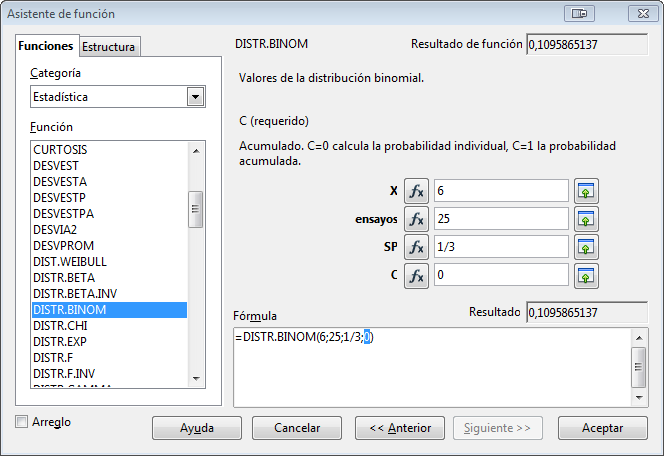
\includegraphics[width=8cm]{../fig/Tut05-19.png}
\end{center}

\begin{ejercicio}
\label{tut05:ejercicio08}
\quad\\
Repite en Calc los cálculos del Ejercicio \ref{tut05:ejercicio02}. O, al menos, repite algunos de ellos y piensa como harías el resto.
\qed
\end{ejercicio}

\subsubsection*{Wiris}

Wiris no ofrece herramientas especiales para trabajar con la distribución binomial. En el fichero adjunto:
\begin{center}
  \fichero{../html/Tut05-BinomialConWiris.html}{Tut05-BinomialConWiris.html}
\end{center}
hemos incluido una sesión de trabajo con Wiris, en la que se calculan valores de probabilidad de una binomial, y que puedes modificar para cubrir tus necesidades. Como en otros casos, una ventaja de trabajar con Wiris es su capacidad de expresar simbólicamente (como fracciones, sin redondeos) algunos resultados.

\begin{ejercicio}
\label{tut05:ejercicio09}
\quad\\
Calcular, usando Geogebra o Wiris, la probabilidad $P(300<X<600)$ si $X\sim B(1000, 1/3)$. Es el Ejemplo \ref{curso-cap05:ejem:DistribucionBinomialProbabilidadIntervalo02} del libro (pág. \pageref{curso-cap05:ejem:DistribucionBinomialProbabilidadIntervalo02}), en el que puedes ver la monstruosa solución exacta. Solución en la página \pageref{tut05:ejercicio09:sol}.
\qed
\end{ejercicio}



\subsubsection*{Wolfram Alpha}

Wolfram Alpha es muy potente, pero el mayor problema suele ser el de encontrar la forma correcta de formular la pregunta. Por ejemplo, para calcular $P(X\leq 6)$ cuando $X\sim B(25, \frac{1}{3})$ puedes usar:
    \begin{center}
    \begin{minipage}{10cm}
    \begin{verbatim}
    Prob x <= 6 if x is binomial with n = 25 and p = 1/3
    \end{verbatim}
    \end{minipage}
    \end{center}
devuelve el resultado correcto, pero si sustituyes {\tt <=} por {\tt =} (para calcular la densidad), Wolfram Alpha no lo entiende... y una forma correcta es esta (mucho menos intuitiva):
    \begin{center}
    \begin{minipage}{10cm}
    \begin{verbatim}
    PDF[BinomialDistribution[25, 1/3], 6]
    \end{verbatim}
    \end{minipage}
    \end{center}
donde {\tt PDF} corresponde a Probability Density Function. No dejes, en cualquier caso, de consultar las páginas de ejemplos de Wolfram Alpha (y una búsqueda astuta en internet a menudo muestra cómo formular la pregunta que nos interesa).

Puedes consultar también esta página web ({\em Binomial Distribution Calculator}, en {\em Wolfram Alpha Widgets}),
\begin{center}
  \link{http://www.wolframalpha.com/widgets/view.jsp?id=78baf4f3a070cc5b9b226664d2ce80ec}{http://www.wolframalpha.com/widgets/view.jsp?id=78baf4f3a070cc5b9b226664d2ce80ec}
\end{center}
que permite usar Wolfram Alpha para cálculos con la binomial, mediante una interfaz bastante más sencilla.

\section{Zoo binomial}

Vamos a recurrir a GeoGebra para explorar las distintas distribuciones binomiales que se obtienen al variar los valores de $n$ y $p$. GeoGebra tiene la ventaja de que nos permite hacer esa exploración dinámicamente, de una forma muy sencilla. Además, como veremos, lo vamos a poder utilizar en más casos a lo largo del curso.

Empezamos abriendo la ventana de GeoGebra (tiene que ser una versión reciente; yo he usado la versión 4.4.39 para este tutorial), y en el menú desplegable de herramientas que se indica en la siguiente figura, seleccionamos la herramienta llamada {\em Calculadora de Probabilidades}.

\begin{center}
    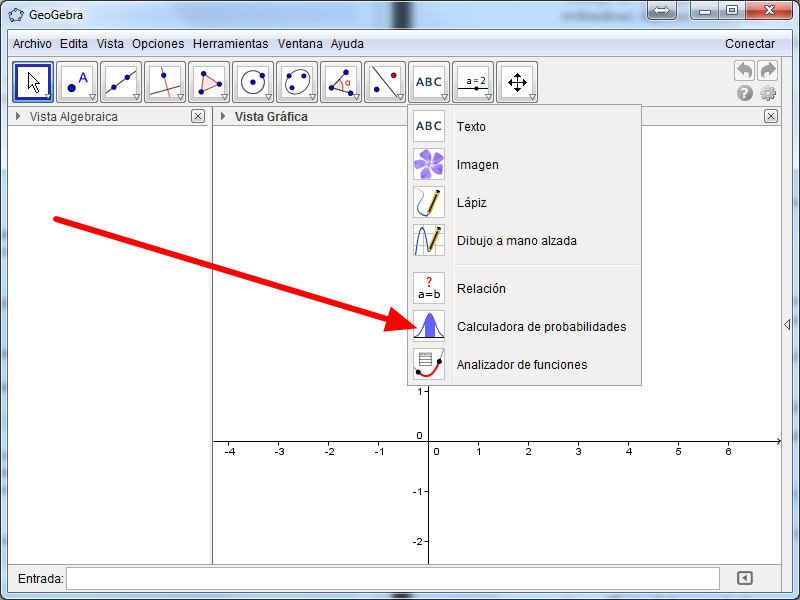
\includegraphics[width=14cm]{../fig/Tut05-22.png}
\end{center}

Al hacer clic sobre esa herramienta se abrirá una nueva ventana. Te recomiendo maximizarla para aprovechar al máximo el espacio de pantalla. Inicialmente, la ventana muestra una curva en forma de campana, que corresponde a la distribución normal (sobre la que volveremos en breve, tanto en el libro como en este tutorial). Como se ve en la siguiente figura, haz clic sobre el menú desplegable de la parte inferior, que nos permite elegir el tipo de distribución con la que vamos a trabajar, y selecciona la Binomial.

\begin{center}
    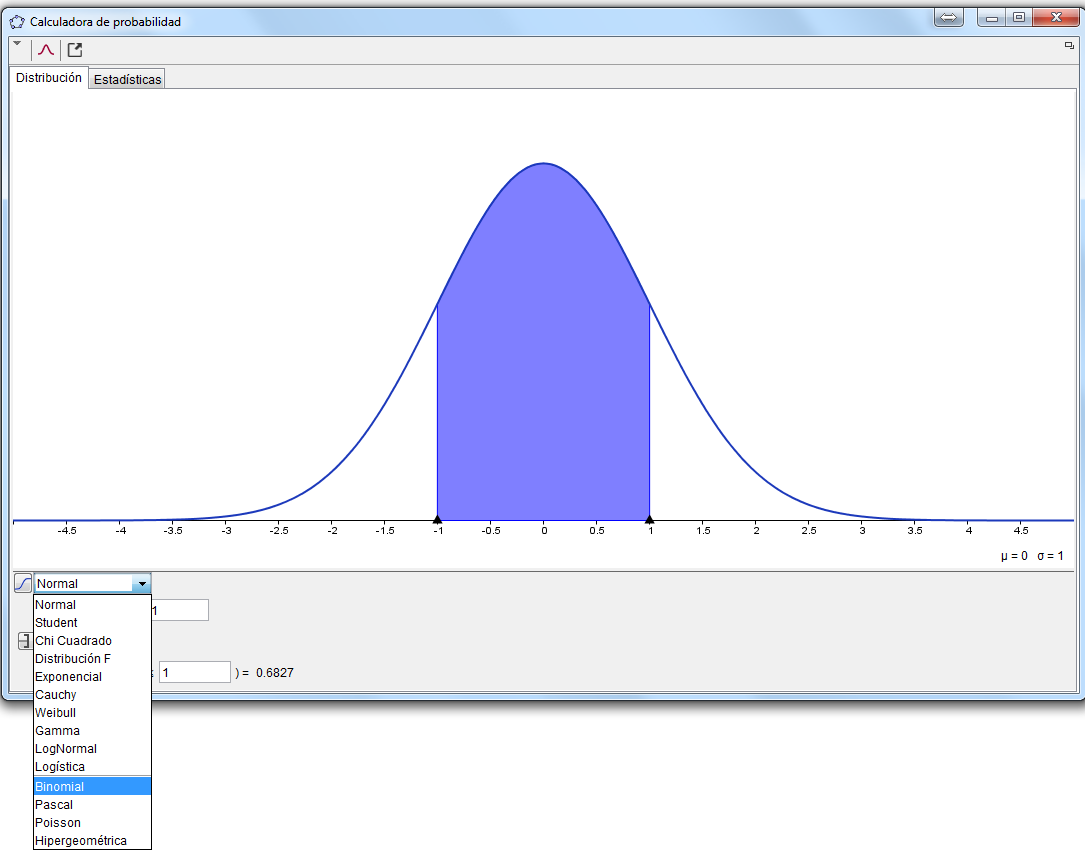
\includegraphics[width=15cm]{../fig/Tut05-23.png}
\end{center}

La ventana cambiará de aspecto, para aparecer como en esta figura:

\begin{center}
    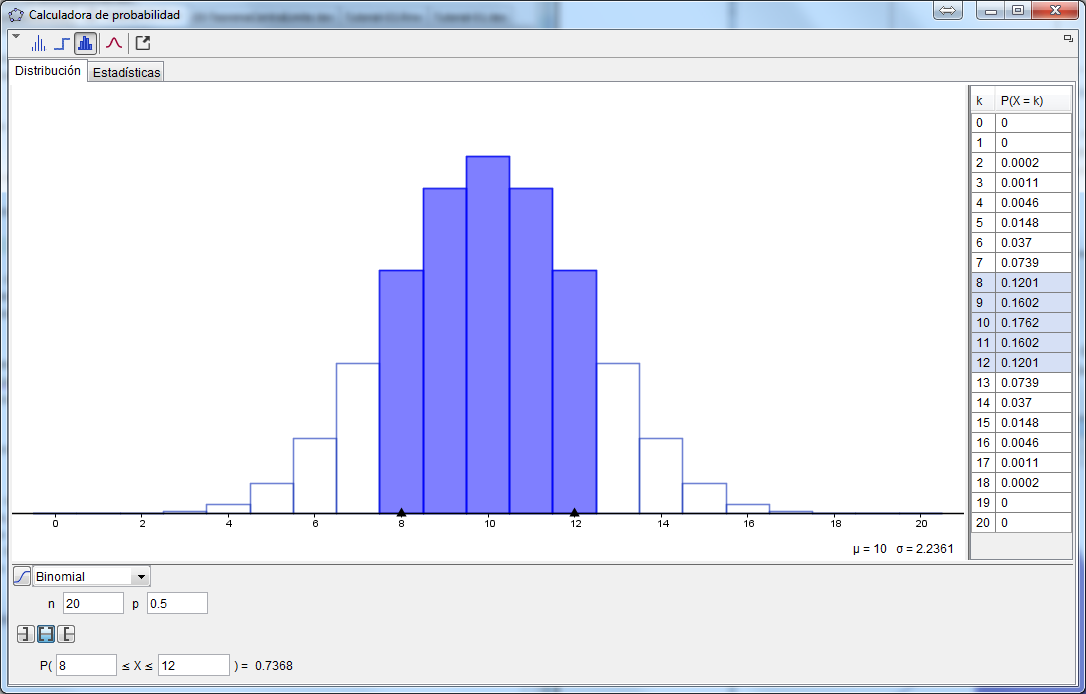
\includegraphics[width=14cm]{../fig/Tut05-24.png}
\end{center}
Esta ventana nos permite usar GeoGebra para hacer cálculos como los del Ejercicio \ref{tut05:ejercicio02} (pág. \pageref{tut05:ejercicio02} de este tutorial), acompañándolos con la interpretación gráfica de lo que estamos calculando. Para usar la herramienta tenemos que introducir los valores de $n$ y $p$, junto con los extremos adecuados del intervalo, en los correspondientes campos de esta ventana. Además, usamos los iconos \begin{center}

\includegraphics[width=2cm]{../fig/Tut05-26.png}
\end{center}
para seleccionar la forma del intervalo que nos interesa,  y que se corresponden, respectivamente, con preguntas de uno de estos tipos:
\[
P(X\leq a),\qquad  P(a\leq X\leq b),\qquad P(X\geq b)
\]
En el caso de la parte 7 del Ejercicio \ref{tut05:ejercicio02} (calcular $P(2\leq X< 4)$ en $X\sim B(7, 1/4)$) , por ejemplo, sería así:
\begin{center}
    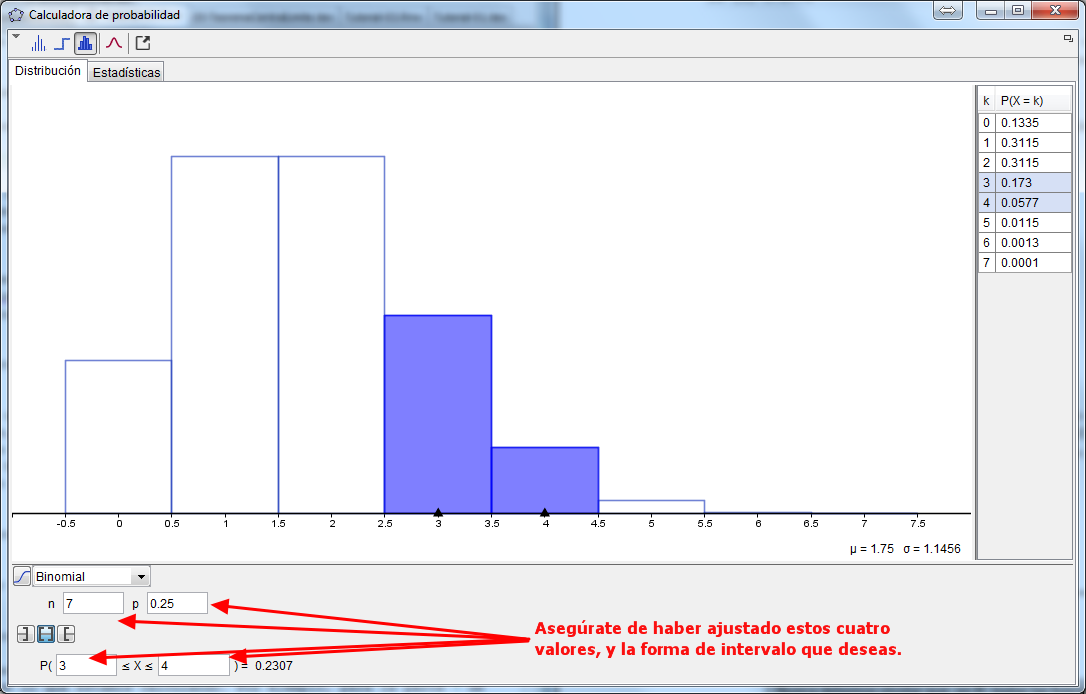
\includegraphics[width=15cm]{../fig/Tut05-25.png}
\end{center}
Ampliación de los campos en los que introducimos los valores:
\begin{center}
    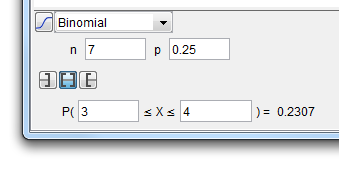
\includegraphics[width=7cm]{../fig/Tut05-27.png}
\end{center}
Como ves, en este caso hemos obtenido la respuesta que esperábamos, $0.2307$. La ventana, además, ilustra mediante un diagrama de columnas los valores de probabilidad que estamos calculando, mientras que, a la derecha y en vertical, puedes ver la tabla de densidad de la variable $X$. Si te fijas, verás que GeoGebra ha incluido en la figura los valores de $\mu$ y $\sigma$. Ya iremos descubriendo algunos elementos adicionales de esta ventana.

\begin{ejercicio}
\label{tut05:ejercicio10}
\quad\\
De nuevo, usa esta herramienta de GeoGebra para reproducir todos los resultados del Ejercicio \ref{tut05:ejercicio02}.
\qed
\end{ejercicio}

Aunque, en principio, la {\em Calculadora de Probabilidades} de GeoGebra nos permite examinar el efecto de utilizar distintos valores de $n$ y $p$, lo podemos hacer mejor volviendo a la interfaz básica del programa. Cierra, por tanto, la {\em Calculadora} y en la ventana principal de GeoGebra selecciona la herramienta {\em deslizador}, haciendo clic en el icono $\begin{array}{l}
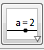
\includegraphics[width=1cm]{../fig/Tut05-28.png}
\end{array}$. Ahora usa esa herramienta, haciendo clic en dos lugares cualesquiera de la vista gráfica, para crear dos deslizadores para $n$ y $p$. Para crearlos hemos usado las opciones que aparecen indicadas por flechas rojas en estas figuras:
\begin{center}
    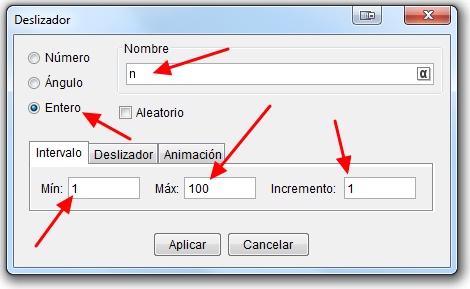
\includegraphics[height=4.5cm]{../fig/Tut05-29a.png}
    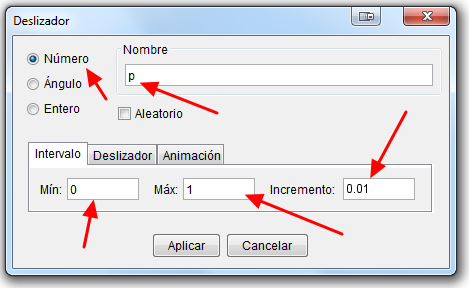
\includegraphics[height=4.5cm]{../fig/Tut05-29b.png}
\end{center}
También puedes crear los deslizadores desde la  {\em Línea de entrada} de GeoGebra (que está en la parte inferior de la ventana principal del programa), ejecutando consecutivamente los comandos:
\begin{center}
{\tt n = Deslizador[1,100,1,0,200]}
\end{center}
y
\begin{center}
{\tt p = Deslizador[0,1,0.01,0,200]}
\end{center}
Una vez creados estos deslizadores, usamos de nuevo la {\em Línea de entrada} y tecleamos (o usamos copia-pega)
\begin{center}
  {\tt DistribuciónBinomial[n,p]}
\end{center}
Inicialmente, puesto que tienes $n=1, p=1$ la figura no te dirá gran cosa. Para hacerlo interesante, usa el ratón para mover los deslizadores de manera que sea $n=20$ y $p=0.25$. Los valores de la probabilidad empiezan a aparecer, pero son poco visibles. El problema, naturalmente, es que al ser valores entre $0$ y $1$, la escala del eje vertical tiene que cambiar para que podamos apreciarlos. Una posibilidad es ejecutar en la {\em Línea de entrada} el siguiente comando:
\begin{center}
  {\tt RazónEjes[25,3]}
\end{center}
Este reajuste de escalas también se puede hacer dinámicamente, usando el ratón. Empieza por hacer clic en el icono $\begin{array}{l}
\includegraphics[width=1cm]{../fig/Tut05-30.png}\end{array}$ situado en el extremo derecho de la barra de herramientas. Ahora, una vez que hayas seleccionado esa herramienta (que GeoGebra llama {\em Desplaza Vista Gráfica}), sitúa el ratón sobre el eje vertical. Cuando esté bien colocado el cursor se convertirá en una doble flecha (y puede aparecer un rótulo {\em EjeY}), como en esta figura:
\begin{center}
    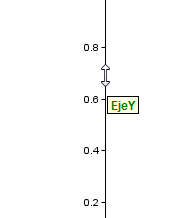
\includegraphics[height=5cm]{../fig/Tut05-31.png}
\end{center}
En ese momento haz clic con el botón izquierdo del ratón y, sin soltarlo, ``estira'' el eje vertical para cambiar su escala. El resultado puede ser algo como lo que se muestra en esta figura.
\begin{center}
    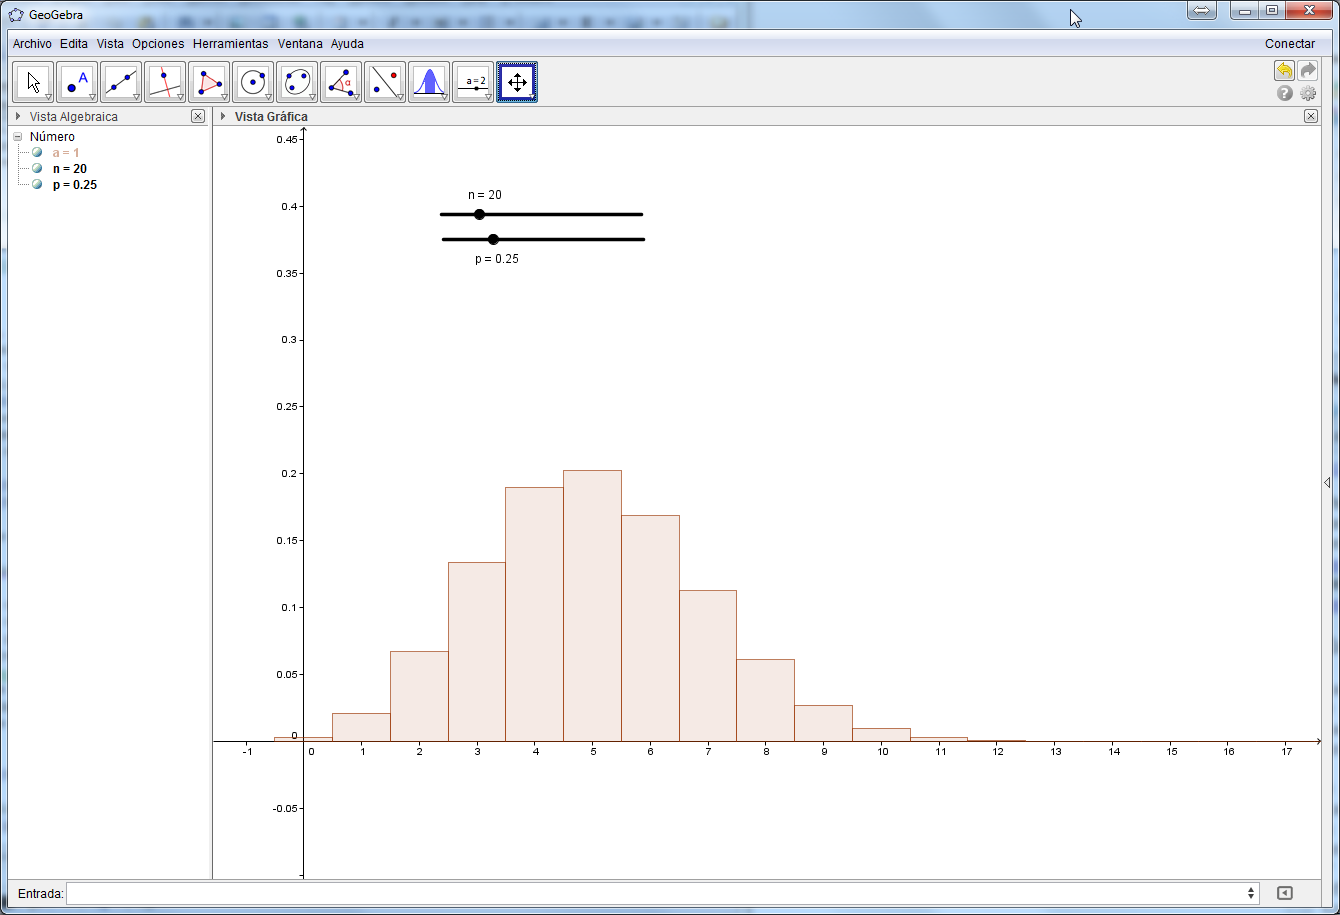
\includegraphics[width=15cm]{../fig/Tut05-32.png}
\end{center}
Recuerda, además, que para desplazar la vista gráfica en GeoGebra basta con hacer click (botón izquierdo) en cualquier zona vacía de la {\em Vista Gráfica} y arrastrar con el ratón, mientras mantienes pulsada la tecla {\tt Ctrl} o la tecla mayúsculas.

Otra posibilidad, una vez que has seleccionado la herramienta {\em Desplaza Vista Gráfica} es hacer clic con el botón derecho en una zona vacía de la gráfica. Debería aparecer el cuadro de diálogo titulado {\em Vista Gráfica}, en el que a su vez puedes seleccionar la opción {\em Vista gráfica}
\begin{center}
    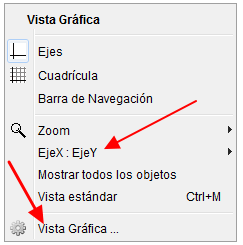
\includegraphics[width=7cm]{../fig/Tut05-33.png}
\end{center}
En ese mismo cuadro de diálogo aparece la opción {\tt EjeX:EjeY}, que te puede servir, pero se limita a ciertos valores prefijados, que no siempre son adecuados a lo que queremos. Tras seleccionar {\em Vista gráfica}, en la ventana que aparece puedes elegir una relación de escalas entre los ejes similar a {\tt 25:1}.
\begin{center}
    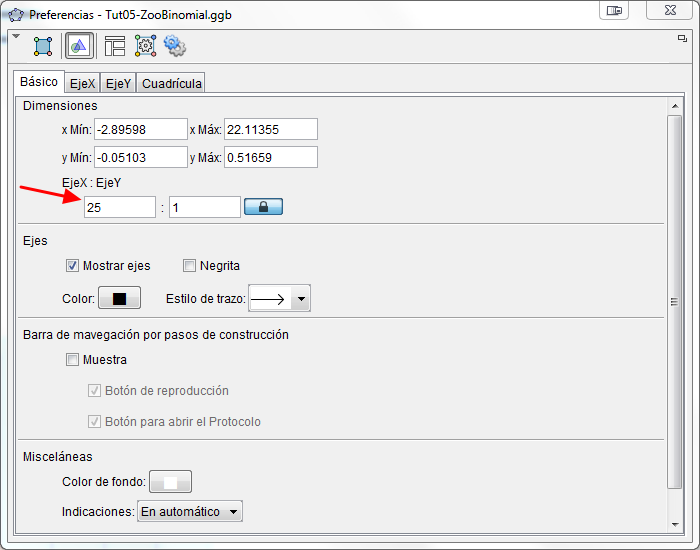
\includegraphics[width=9cm]{../fig/Tut05-34.png}
\end{center}
y cerrar esta ventana para volver a la vista gráfica.  En cualquier caso, por si tienes problemas para ajustar la escala de los ejes, aquí tienes adjunto el fichero
\begin{center}
  \fichero{../ggb/Tut05-ZooBinomial.ggb}{Tut05-ZooBinomial.ggb}
\end{center}
que debería abrirse en GeoGebra mostrando una escala del eje vertical adecuada para que puedas experimentar.

Porque esa es la clave de todo este trabajo de preparación. El objetivo es que juegues con los deslizadores $n$ y $p$ y observes la forma de la distribución de probabilidad. En la Sección \ref{curso-cap05:subsec:ZooDistribucionesBinomiales} (pág. \pageref{curso-cap05:subsec:ZooDistribucionesBinomiales}) del libro se describen, a grandes rasgos, tres posibles situaciones que pueden darse en las distribuciones binomiales. Trata de jugar con los valores de $n$ y $p$ hasta asegurarte de que has pasado por esas tres situaciones (para valores de $n$ mayores que $30$ es posible que quieras hacer zoom para mejorar la visualización; la rueda del ratón te servirá para esto). La intuición que adquieras sobre el comportamiento de la binomial nos será muy útil para el trabajo de este y los próximos capítulos.

\begin{ejercicio}
\label{tut05:ejercicio11}
\begin{enumerate}
  \item[]
  \item Reproduce, usando los deslizadores $n$ y $p$ las distribuciones binomiales que aparecen en la Figura \ref{curso-cap01:fig:ZooBinomial01} del libro (pág. \pageref{curso-cap01:fig:ZooBinomial01}). Si quieres reproducir la Figura \ref{curso-cap01:fig:ZooBinomial04} (o alguna otra binomial fuera del rango de los deslizadores), lo más fácil es que abras una nueva ventana de GeoGebra y utilices directamente el comando {\tt DistribuciónBinomial[10000,0.0001]} (en la {\em Línea de Entrada}), además de ajustar la escala de los ejes como hemos descrito.

  \item Usa la {\em Calculadora de Probabilidades} de GeoGebra para reproducir el resultado que ilustra la Figura \ref{curso-cap05:fig:HistogramaBinomial05} del libro (pág. \pageref{curso-cap05:fig:HistogramaBinomial05}).
\end{enumerate}
\qed
\end{ejercicio}

\section{Variables aleatorias continuas. Funciones e integración con GeoGebra, Wiris y Wolfram Alpha.}
\label{tut05:sec:IntegracionWirisWolfram}


%Al comenzar el trabajo con funciones continuas, vamos a echar mano de muchas herramientas propias de la parte de la Matemáticas que se denomina Cálculo. El Cálculo estudia las funciones, y uno de los objetivos habituales de un curso tradicional de Cálculo es el estudio de las gráficas de las funciones. Antes de la aparición de los ordenadores, el dibujo aproximado de la gráfica de una función era una  tarea esencialmente manual, guiada por los resultados que se obtenían usando el Cálculo.
%
%Con los ordenadores y los programas gráficos que permiten dibujar funciones fácilmente, las cosas se han simplificado mucho. Naturalmente, no estamos sugiriendo que los ordenadores

En este apartado vamos a aprender a usar algunas de las herramientas que ya conocemos para trabajar con las funciones que usaremos en el estudio de las distribuciones continuas. Para empezar, vamos a practicar el dibujo de gráficas.

\subsection{Gráficas de funciones.}

Para aprovechar la inercia de la Sección anterior, vamos a empezar usando GeoGebra para la representación de funciones de la forma $y = f(x)$. Por ejemplo, vamos a dibujar la función que aparece en el Ejemplo \ref{curso-cap05:ejem:CalculoProbabilidadIntegralParte1} del libro (pág. \pageref{curso-cap05:ejem:CalculoProbabilidadIntegralParte1}).
\[
y = \dfrac{1}{\pi(1+x^2)}
\]
Abre una ventana nueva de GeoGebra (cierra y vuelve a abrir el programa si es necesario) y teclea o copia, en la {\em Línea de Entrada}, este comando:
\begin{center}
  \verb&f(x) = 1 / (Pi * (1 + x^2))&
\end{center}
Como ves, es una sintaxis muy parecida a la de R, o Wolfram Alpha (o muchos otros programas de Matemáticas). Hay que usar juiciosamente los paréntesis pero, aparte de eso, la única peculiaridad es que GeoGebra reconoce el símbolo {\tt Pi} (y también {\tt pi} en minúsculas) para indicar la constante $\pi$. Por ejemplo, en R, sólo funciona {\tt pi} en minúsculas. Wolfram Alpha normalmente entiende cualquiera de las dos. Ese tipo de detalles cambian de un programa a otro, pero la mayor parte de la sintaxis se mantiene. Y eso facilita muchas veces el mover información de un programa a otro. Uno de los mensajes que queremos transmitir en estos tutoriales es que las herramientas basadas en texto son, en general, más {\em productivas}, una vez se superan las dificultades iniciales.

Pero, en cualquier caso, cuando uses herramientas basadas en texto para trabajar con funciones, recuerda que estás haciendo una traducción desde la notación matemática habitual a esa notación basada en texto. Es, por tanto, muy importante que te asegures de que la traducción ha sido correcta, y de que estás de hecho trabajando con la función que te interesa. En GeoGebra, por ejemplo, la {\em Vista Algebraica} te mostrará la función que has introducido en una notación más parecida a la notación matemática habitual.

Cuando hayas ejecutado ese comando GeoGebra, la {\em Vista Gráfica} tendrá un aspecto similar a este:
\begin{center}
    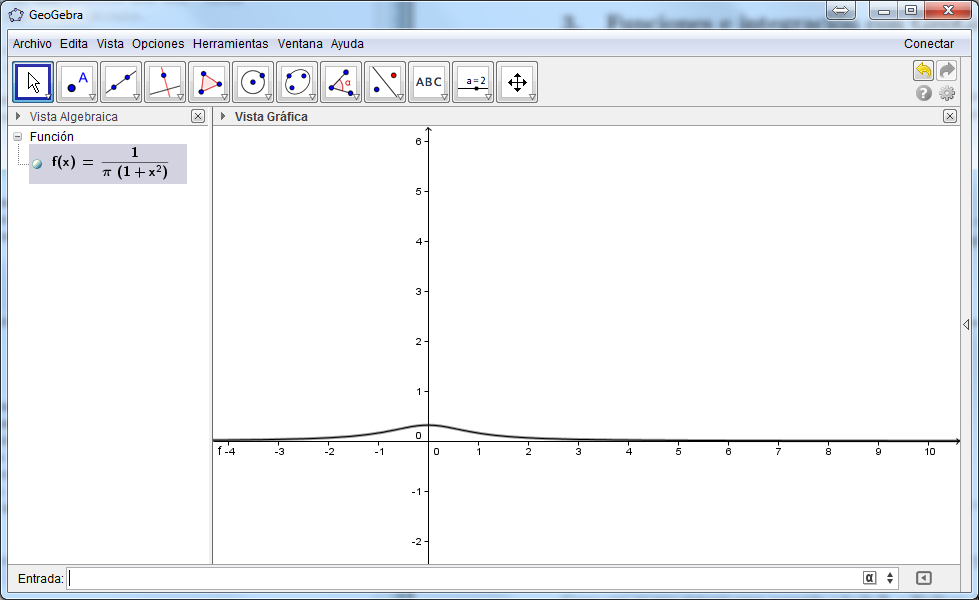
\includegraphics[width=15cm]{../fig/Tut05-35.png}
\end{center}

Es un buen momento para que practiques con esta figura, ajustando escalas, posición, etc. Experimenta un poco con la gráfica. En este curso nos vamos a limitar a cubrir el conocimiento mínimo necesario sobre funciones. Pero si necesitas más, la documentación de GeoGebra es muy amplia, y la información disponible en la red sobre ese programa es ingente.

Pasando a Wolfram Alpha, prueba a copiar exactamente el mismo comando en el campo de entrada del programa. El comienzo del resultado al ejecutarlo es este:
\begin{center}
    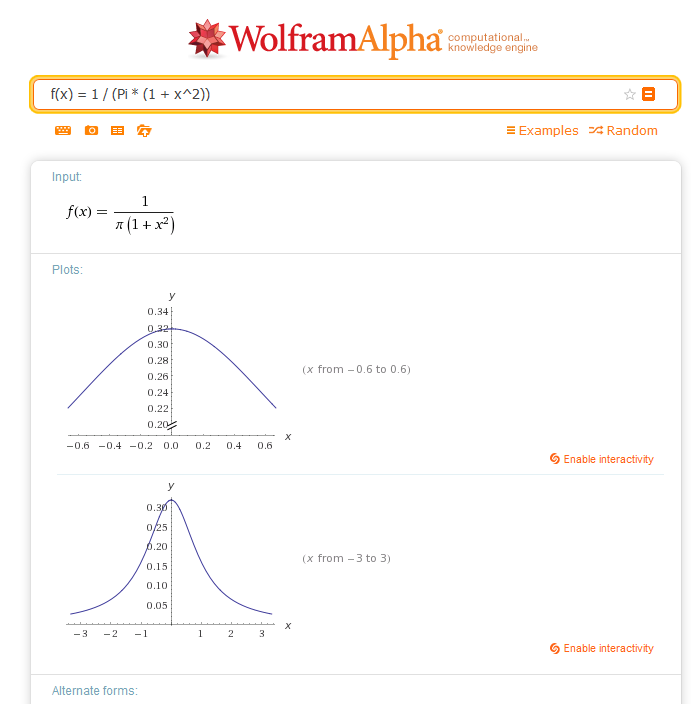
\includegraphics[width=13cm]{../fig/Tut05-36.png}
\end{center}
Además de un par de gráficas a distintas escalas (y de la función en notación matemática, que siempre conviene chequear para ver que el programa nos ha entendido), Wolfram Alpha nos proporciona, como de costumbre, mucha información adicional sobre esta función. Puedes explorarla, para hacerte una idea de lo que obtenemos (por ejemplo, una primitiva).

\begin{ejercicio}
\label{tut05:ejercicio12}
\quad\\
Dibuja la gráfica de las siguientes funciones, usando tanto GeoGebra como Wolfram Alpha:
\begin{enumerate}
    \item La distribución normal de la Ecuación \ref{curso-cap05:ecu:EcuacionCurvaNormal} del libro (pág. \pageref{curso-cap05:ecu:EcuacionCurvaNormal}), para $\mu = 0$, $\sigma = 1$.
    \item Una parábola muy sencilla, $f(x)=x^2$. Después, dibuja (1) $f_1(x)=-x^2$, (2) $f_2(x)=(x-1)^2$,     (3) $f_3(x)=(x+1)^2$, (4) $f_4(x)= 2\cdot x^2$ (5) $f_5(x) = \dfrac{1}{2}x^2$.
\end{enumerate}
El objetivo del anterior ejercicio, como el de este, es hacerte pensar sobre lo que sucede con la gráfica de una función $y= f(x)$ al hacer un cambio de variable de la forma
        \[y = c\cdot f(a\cdot x + b),\]
donde $a, b$ y $c$ son constantes.
\begin{enumerate}\setcounter{enumi}{2}
    \item Para profundizar en esto vamos a usar los deslizadores de GeoGebra. Abre una nueva ventana de GeoGebra y escribe, uno por uno, estos comandos:
        \begin{center}
          {\tt a = Deslizador[-10,10,0.1,0,200]}\\
          {\tt a = 1}\\
          {\tt b = Deslizador[-10,10,0.1,0,200]}\\
          {\tt c = Deslizador[-10,10,0.1,0,200]}\\
          {\tt c = 1}
        \end{center}
        Con esto hemos definido tres deslizadores, cuyo recorrido va de $-10$ a $10$, en incrementos de $0.1$, y hemos fijado el valor inicial de $a$ y $c$ a $1$ (el valor inicial de $b$ es $0$). No te preocupes por las dos últimas opciones del comando  {\tt Deslizador}, que no vamos a usar. Naturalmente, también puedes usar el icono $\begin{array}{l}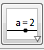
\includegraphics[width=1cm]{../fig/Tut05-28.png}\end{array}$ de la {\em Barra de Herramientas}. Ahora ejecuta el comando:
        \begin{center}
          {\tt f(x) = c * sen(a * x + b)}
        \end{center}
        En ese momento, el aspecto de la ventana gráfica debe ser similar a este:
        \begin{center}
        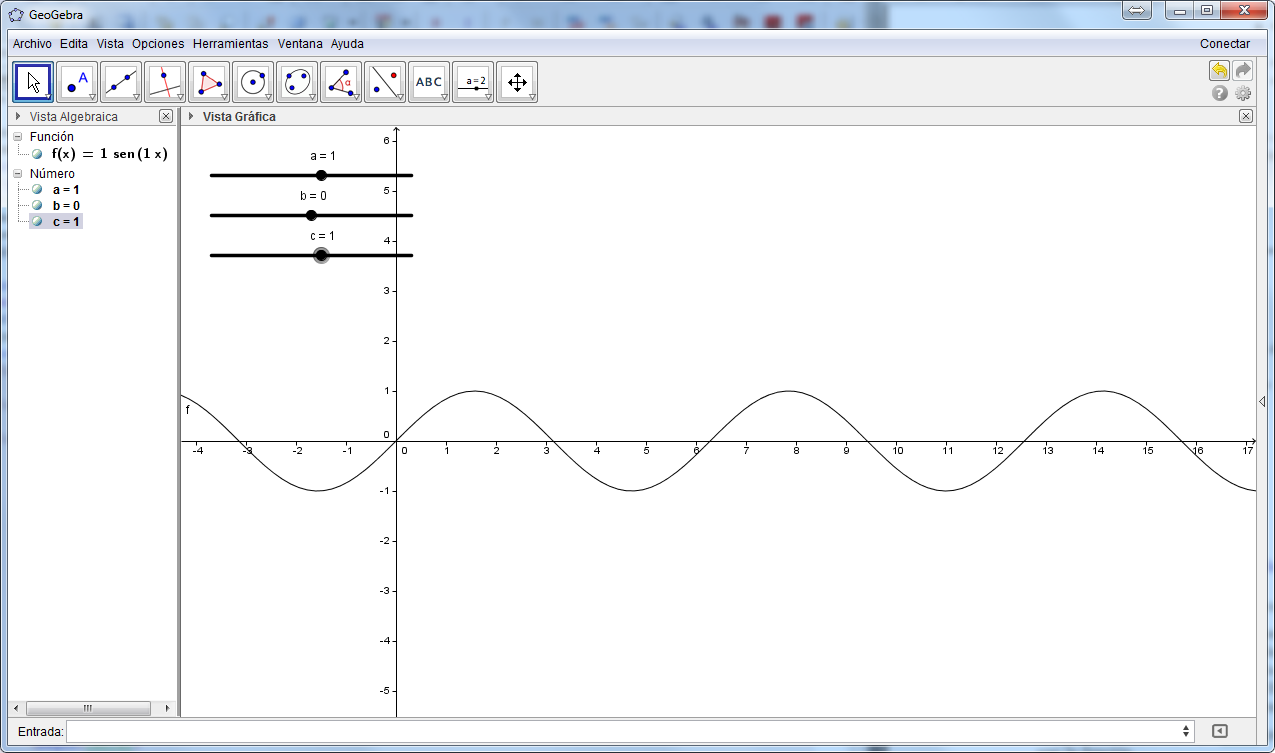
\includegraphics[width=15cm]{../fig/Tut05-37.png}
        \end{center}
        Prueba a manipular los deslizadores para ver el efecto que los cambios en $a, b$ y $c$ tienen sobre la gráfica. Los tres efectos que se observan son fáciles de traducir en palabras. Inténtalo.
    \item Hay un cuarto efecto que puedes analizar, para el que vamos a añadir un deslizador adicional, llamado $d$, que corresponde a esta fórmula:
        \[y = c\cdot f(a\cdot x + b) + d.\]
        Usa el ejemplo de la función seno para añadir un deslizador más, que represente el valor de $d$, y estudiar su efecto en la gráfica. Tendrás que redefinir la función $f$ en GeoGebra, usando de nuevo la {\em Línea de Entrada}.

\end{enumerate}
\qed
\end{ejercicio}

\subsection{Integrales y sumas de áreas de rectángulos.}
\label{tut05:subsec:IntegralesSumaAreasRectangulos}

La Figura \ref{curso-cap05:fig:IntegralRectangulosSumaInferior} del libro (pág. \pageref{curso-cap05:fig:IntegralRectangulosSumaInferior}) trata de ilustrar que la idea de integral aparece al pensar en la aproximación del área bajo una curva mediante la suma del área de muchos rectángulos inscritos bajo esa gráfica. Esa figura se ha obtenido con el fichero GeoGebra
\begin{center}
  \fichero{../ggb/Tut05-IntegralRectangulosSumaInferior.ggb}{Tut05-IntegralRectangulosSumaInferior.ggb}
\end{center}
que, además, nos va a permitir explorar de forma dinámica lo que ocurre con esas aproximaciones cuando $n$ aumenta. Al abrir el fichero te encontrarás en la {\em Vista Gráfica} una situación parecida a esta:
\begin{center}
    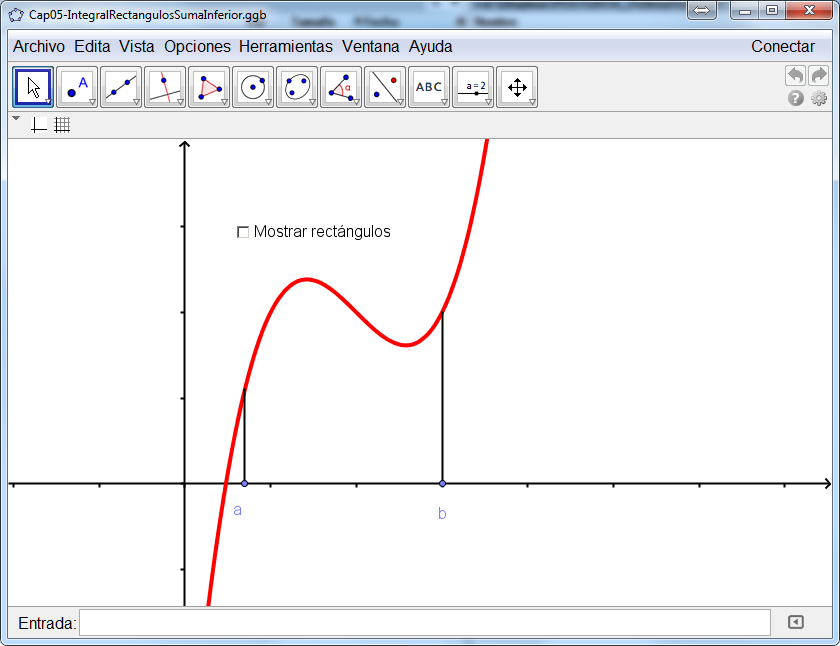
\includegraphics[width=15cm]{../fig/Tut05-38.png}
\end{center}
Haz clic sobre la casilla rotulada {\em Mostrar rectángulos}, para hacer aparecer unos rectángulos inscritos bajo la gráfica de $f$ (inicialmente $2$), y un deslizador que controla el número de rectángulos. En la Figura \ref{curso-cap05:fig:IntegralRectangulosSumaInferior} ese deslizador se ha usado para obtener $15$ rectángulos. Experimenta con ese deslizador, para que veas lo que sucede con el área de los rectángulos a medida que aumenta su número. En la siguiente figura hemos hecho zoom y desplazado la gráfica para que veas con un poco más de detalle lo que sucede cuando usamos $100$ rectángulos:
\begin{center}
    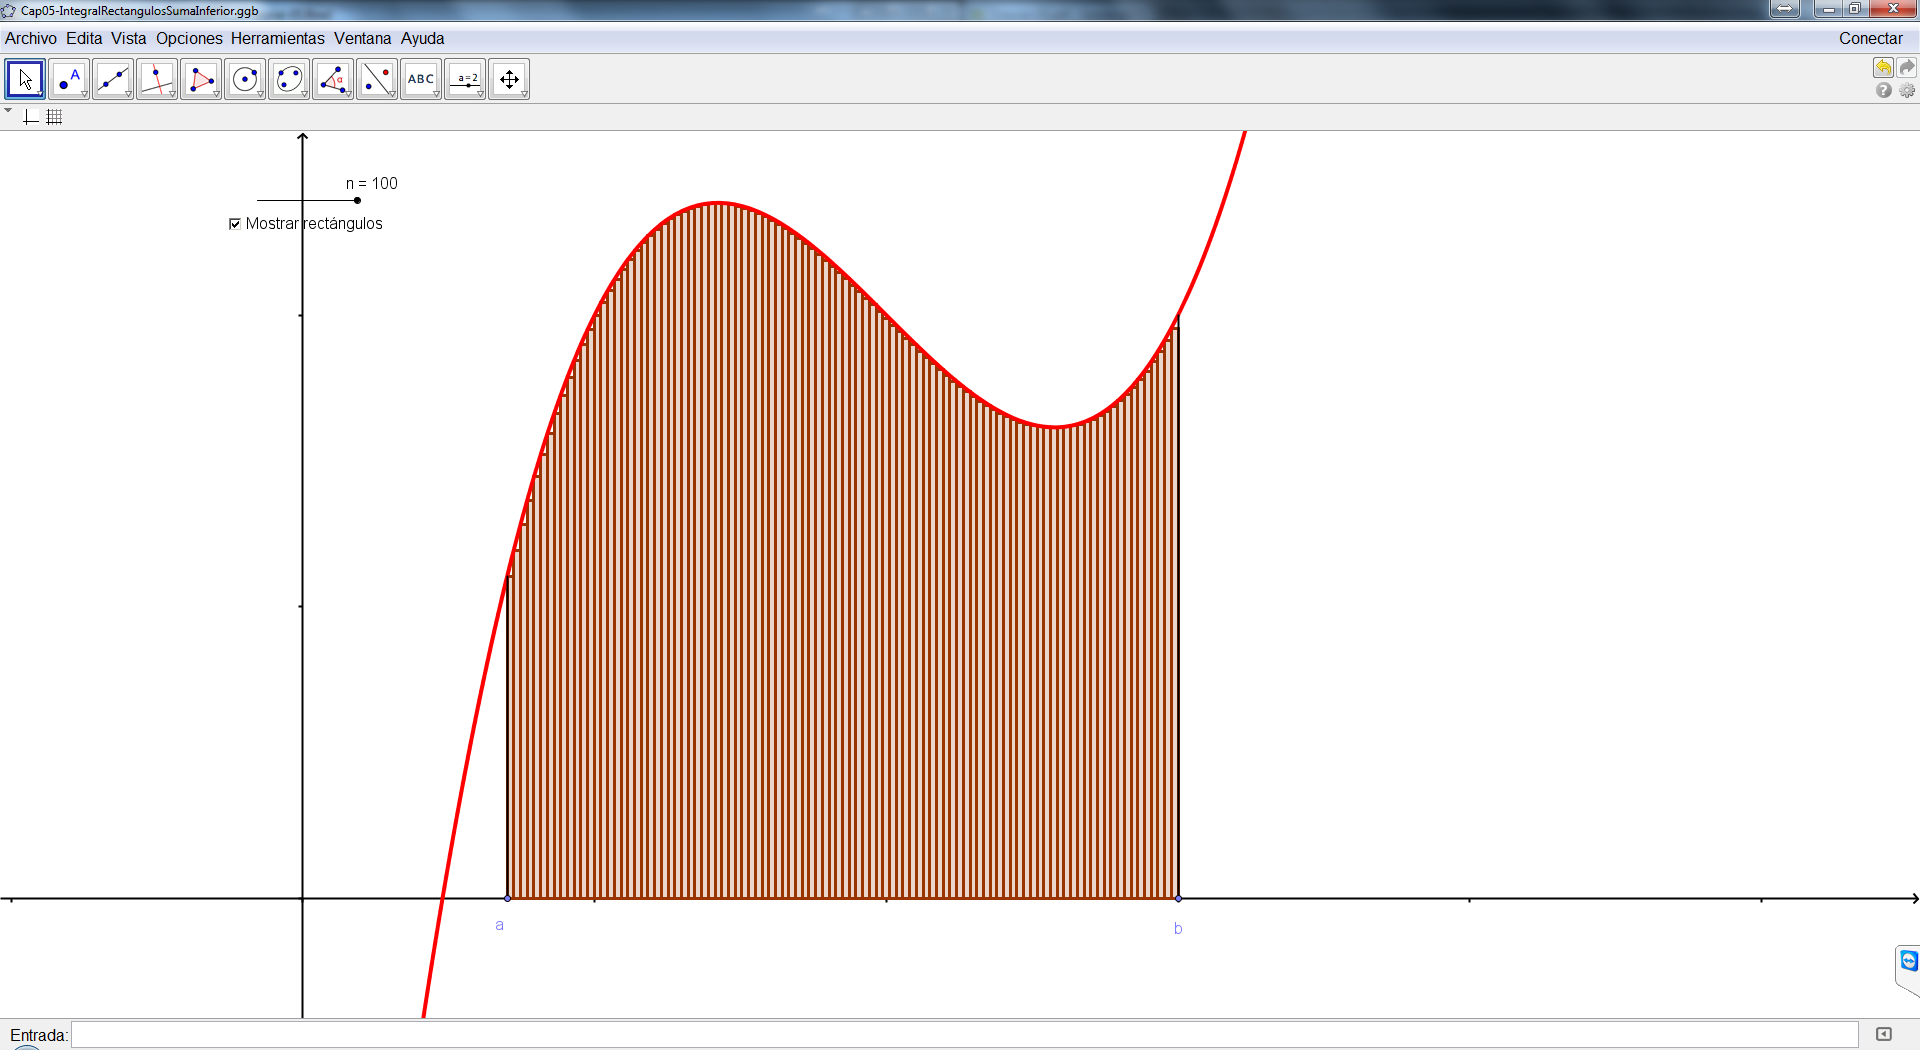
\includegraphics[width=15cm]{../fig/Tut05-39.png}
\end{center}
La diferencia entre la suma del área de los rectángulos y el área bajo la gráfica es, como ves, muy pequeña. Por si deseas usarlo para otros experimentos, el comando de GeoGebra que hemos usado para dibujar esos rectángulos es {\tt SumaInferior}. Puedes buscarlo en la ayuda de la página \link{http://www.geogebra.org}{www.geogebra.org}.

\subsection{Cálculo de áreas y primitivas con GeoGebra, Wolfram Alpha y Wiris.}
\label{tut05:subsec:IntegralesSumaAreasRectangulos}

En el Capítulo \ref{curso-cap:TeoremaCentralLimite} del libro se discute que, para trabajar con variables aleatorias continuas, es necesario el cálculo de áreas mediante integrales, y que una de las herramientas básicas para hacer esto es el cálculo de primitivas. Tradicionalmente, el cálculo manual de primitivas ha venido siendo una de las partes más impopulares del estudio de las Matemáticas. Afortunadamente, la aparición de los sistemas de cálculo computacional (tanto simbólicos como numéricos) hacen que la parte más complicada de esos cálculos podamos dejarla, casi siempre, en manos del ordenador. Desde luego, así va a ser en este curso. En esta sección vamos a ver como usar GeoGebra, Wiris y Wolfram Alpha para resolver algunos de los problemas que hemos ido encontrando en ese capítulo.

\subsubsection{Un primer ejemplo usando integrales.}
\label{tut05:subsubsec:UnPrimerEjemploUsoIntegrales}

Vamos a empezar con un ejemplo muy sencillo, que no está directamente relacionado con el cálculo de probabilidades, pero que nos servirá para hacernos una idea de lo que vamos a hacer. Consideramos la parábola $y= x^2$, y queremos calcular el área que queda debajo de esta parábola y por encima del eje $x$, entre los puntos de coordenadas $x=1$ y $x=2$. El problema se ilustra en esta figura, obtenida con GeoGebra (puedes ver que, de hecho, GeoGebra nos adelanta la respuesta aproximada, que es $2.333$):
\begin{center}
    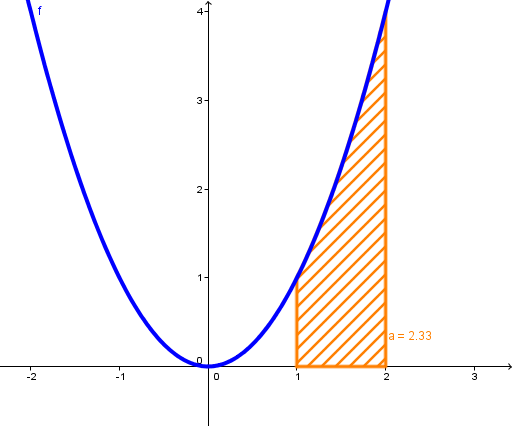
\includegraphics[width=14cm]{../fig/Tut05-40.png}
\end{center}
Para situarlo en un contexto histórico, podemos decir que este problema es, seguramente, el tipo más complicado de problemas de áreas que los matemáticos griegos de la era clásica consiguieron resolver, y que desde ellos hasta Newton no se produjeron grandes avances en ese problema.

Para nosotros las cosas son extremadamente sencillas. Por ejemplo, usando Wolfram Alpha podemos hacer:
\begin{center}
  {\verb&integrate x^2 from 1 to 2&}
\end{center}
y obtenemos la respuesta que se muestra en la siguiente figura:
\begin{center}
    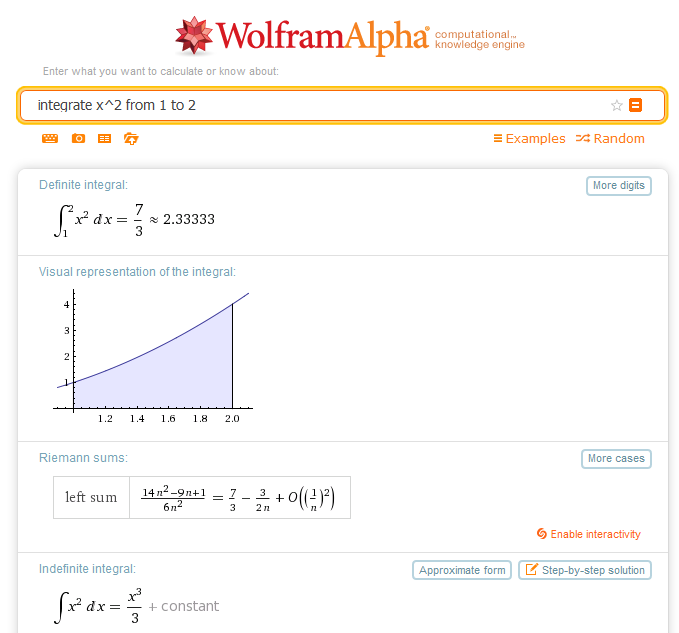
\includegraphics[width=15.5cm]{../fig/Tut05-41.png}
\end{center}
Como ves, el resultado es $\dfrac{7}{3}\approx 2.3333$, como esperábamos. Además, Wolfram Alpha nos proporciona también una primitiva de $f(x)$, en el bloque titulado {\em Indefinite Integral}. Concretamente:
\[F(x) = \int x^2 dx = \dfrac{x^3}{3} + c\]
siendo $c$ una constante. Esta primitiva nos sirve para obtener por otro medio la integral (el área) anterior, usando la Ecuación \ref{curso-cap05:ecu:TeoremaFundamentalCalculo} del libro (pág. \pageref{curso-cap05:ecu:TeoremaFundamentalCalculo}) en lo que se conoce como Regla de Barrow:
\[
\int_1 ^2 f(x) = F(2) - F(1) =
\left(\dfrac{2^3}{3} + c\right) - \left(\dfrac{1^3}{3} + c\right)=
\]
(como ves la constante $c$ se cancela en este cálculo)
\[= \dfrac{8}{3}- \dfrac{1}{3} = \dfrac{7}{3},\]
como ya nos había dicho Wolfram Alpha.

En GeoGebra, para conseguir lo mismo vamos a usar una nueva herramienta, llamada {\em Cálculo Simbólico (CAS)}. La encontrarás en el menú {\em Vista}, como indica esta figura:
\begin{center}
    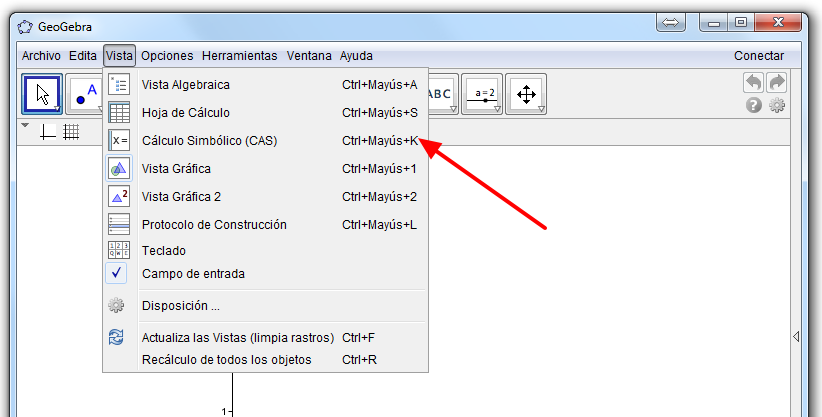
\includegraphics[width=15cm]{../fig/Tut05-42a.png}
\end{center}
Al usar esta opción, en la ventana de GeoGebra aparecerá un nuevo panel. Te aconsejo que maximices la pantalla para disponer de espacio suficiente. Sitúate en el campo indicado con un $1$, teclea \verb#x^2# y {\bf todavía no pulses {\tt Entrar}}. Tu ventana tendrá este aspecto (sólo se muestra una parte):
\begin{center}
    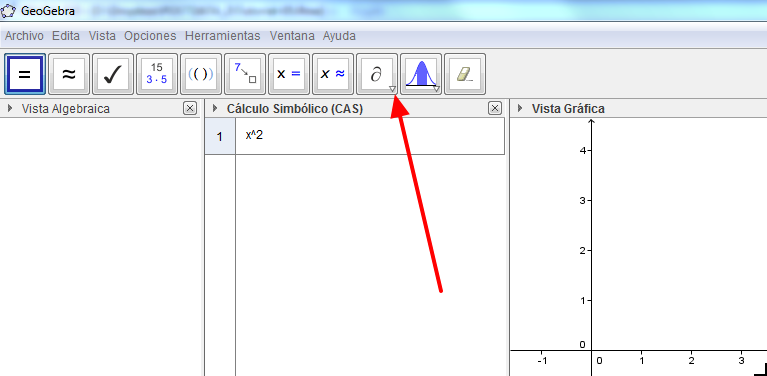
\includegraphics[width=15cm]{../fig/Tut05-43.png}
\end{center}
{\bf Ahora hay que ir con cuidado:} haz clic en el pequeño triángulo de la esquina inferior derecha del icono $\begin{array}{l}
\includegraphics[width=1cm]{../fig/Tut05-44.png}\end{array}$ de la {\em Barra de Herramientas}. Tiene que ser en el triángulo para desplegar el menú, porque si haces clic directamente en elcentro del  icono, calcularás la derivada en lugar de la primitiva, y tendríamos que volver atrás. Cuando aparezca el menú desplegable haz clic en la opción {\em Integral}, del icono $\begin{array}{l}
\includegraphics[width=1cm]{../fig/Tut05-45.png}\end{array}$. El resultado debería ser similar a este:
\begin{center}
    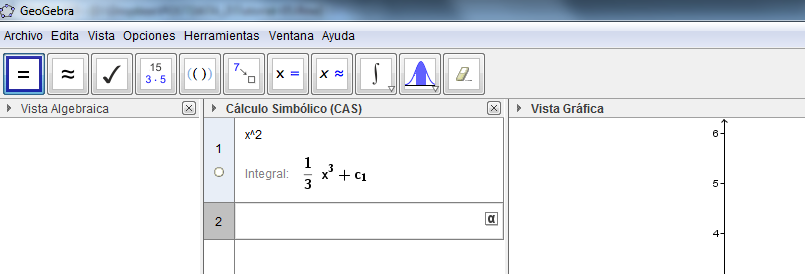
\includegraphics[width=15cm]{../fig/Tut05-46.png}
\end{center}
Puedes usar copiar y pegar (botón derecho del ratón, recuerda) para trasladar el resultado a otros programas, con las precauciones sintácticas habituales en esos casos.
GeoGebra, como ves, es un poco más complicado de usar que Wolfram Alpha para el cálculo de primitivas. A cambio, puedes utilizarlo sin conexión a internet, y nos consta que cada nueva versión ha supuesto una mejora considerable en las posibilidades de uso del programa (en el momento de escribir esto, estamos esperando la versión 5 que, por ejemplo, incluirá gráficos tridimensionales).

En las próximas secciones vamos a usar también Wiris para algunas de estas operaciones, y explicaremos cómo se calculan las primitivas en ese programa.

\subsubsection{Una función de densidad de una variable continua.}

Empecemos con el Ejemplo \ref{curso-cap05:ejem:CalculoProbabilidadIntegralParte1} del libro (pág. \pageref{curso-cap05:ejem:CalculoProbabilidadIntegralParte1}), en el que hemos dejado pendiente la tarea de verificar que la función
\[f(x)=\dfrac{1}{\pi(1+x^2)}\]
satisface
\[\int_{-\infty}^{\infty}f(x)dx=1\]
(Ver también el Ejemplo \ref{curso-cap05:ejem:DistribucionCauchyIntegralTotal1}, pág. \pageref{curso-cap05:ejem:DistribucionCauchyIntegralTotal1}). Para comprobar esto, empezaremos usando Wiris. Ve a la pestaña {\tt Análisis} y, utilizando el icono $\begin{array}{l}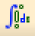
\includegraphics[width=1cm]{../fig/Tut05-13.png}\end{array}$ y otros símbolos que ya conoces, escribe la fórmula como se ve en la siguiente figura (necesitarás $\pi$ y los símbolos de infinito positivo y negativo, de la pestaña {\tt Símbolos}; no confundas $\pi$ con la letra del mismo nombre de la pestaña {\tt Griego}).
\begin{center}
    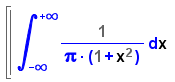
\includegraphics[width=3cm]{../fig/Tut05-14.png}
\end{center}
No olvides el símbolo de producto entre $\pi$ y el paréntesis del denominador, ni la variable $x$ en $dx$. Después pulsa sobre el símbolo igual, y en unos segundos, Wiris te confirmará que el resultado de la integral es, como esperábamos, 1.
\begin{center}
    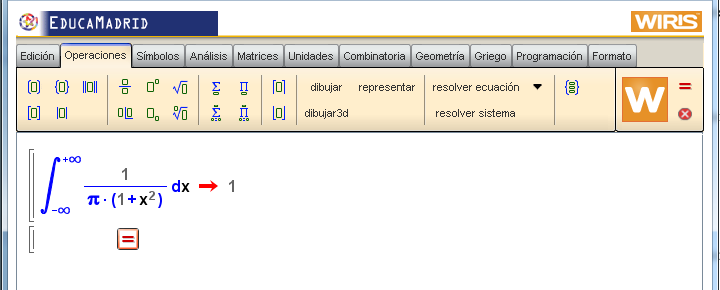
\includegraphics[width=15cm]{../fig/Tut05-47.png}
\end{center}
Para hacer lo mismo con Wolfram Alpha, teclea en el campo de entrada,
    \begin{center}
    \begin{minipage}{10cm}
    \begin{verbatim}
    integrate( 1/( Pi*(1+x^2) ) ) from -Infinity to Infinity
    \end{verbatim}
    \end{minipage}
    \end{center}
y, de nuevo, en unos instantes tendrás la confirmación del resultado, como se ve en esta figura.
\begin{center}
    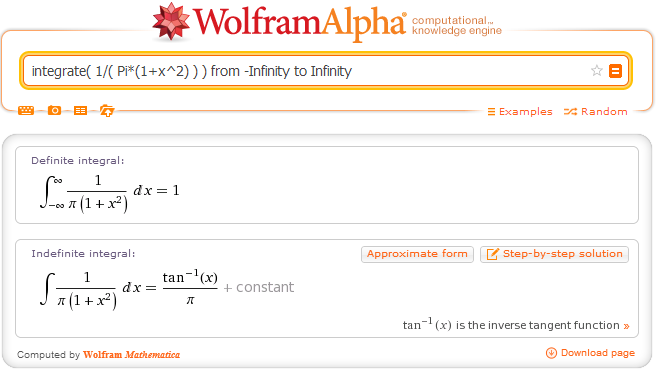
\includegraphics[width=12cm]{../fig/Tut05-15.png}
\end{center}
De hecho, Wolfram Alpha nos da más información de lo que hemos pedido, y nos resuelve la siguiente tarea que dejamos pendiente en el libro: la búsqueda de una primitiva (o integral indefinida) de $f(x)$. Como puede verse en la anterior figura, Wolfram Alpha nos informa de que esa primitiva es
    \[\int\dfrac{1}{\pi\cdot(1+x^2)} dx = \dfrac{\tan^{-1}(x)}{\pi}+constant\]
En esta notación (algo confusa) el símbolo $\tan^{-1}$ se refiere al arcotangente (que, en otros programas, se representa con menos ambigüdad mediante {\tt atan}). Para obtener esa primitva en Wiris vuelve a la pestaña análisis, selecciona esta vez el símbolo (integral sin límites, o indefinida)
\begin{center}
    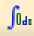
\includegraphics[width=1cm]{../fig/Tut05-16.png}
\end{center}
y úsalo (puedes copiar y pegar trozos de la anterior integral, para facilitarte el trabajo), para obtener el mismo resultado expresado de otra manera:
\begin{center}
    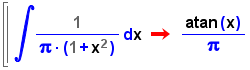
\includegraphics[width=5cm]{../fig/Tut05-17.png}
\end{center}
(Wiris toma 0 como valor de la constante que aparece en Wolfram Alpha). Y para terminar el recorrido por los programas que venimos usando, en en el panel de cálculo simbólico de GeoGebra podemos comprobar el resultado de la integral con el comando:
        \begin{center}
        \verb#Integral[1 / (pi * (1 + x^2)), #$-\infty, \infty${\tt ]}
        \end{center}
mientras que la primitiva se obtiene así:
\begin{center}
    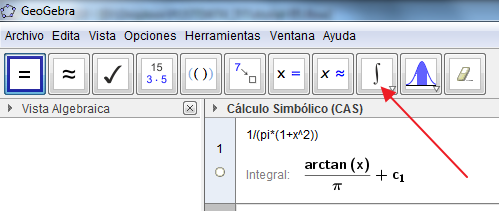
\includegraphics[width=10cm]{../fig/Tut05-48.png}
\end{center}

\subsubsection{Probabilidad de un intervalo.}

Para completar los resultados de los Ejemplos \ref{curso-cap05:ejem:CalculoProbabilidadIntegralParte1} y \ref{curso-cap05:ejem:CalculoProbabilidadIntegralParte2} del libro (pág. \pageref{curso-cap05:ejem:CalculoProbabilidadIntegralParte1}), todavía tenemos que calcular la probabilidad del intervalo $[0,1]$. Es decir:
    \[
    P(0\leq X\leq 1)=\int_0^1f(x)dx=\int_0^1\dfrac{1}{\pi(1+x^2)}dx,
    \]
Vamos a empezar esta vez por GeoGebra. Escribe y ejecuta en la {\em Línea de Entrada} el siguiente comando:
\begin{center}
  \verb#Integral[1 / (pi * (1 + x^2)), 0, 1]#
\end{center}
El resultado se muestra gráficamente, como ves en la figura:
\begin{center}
    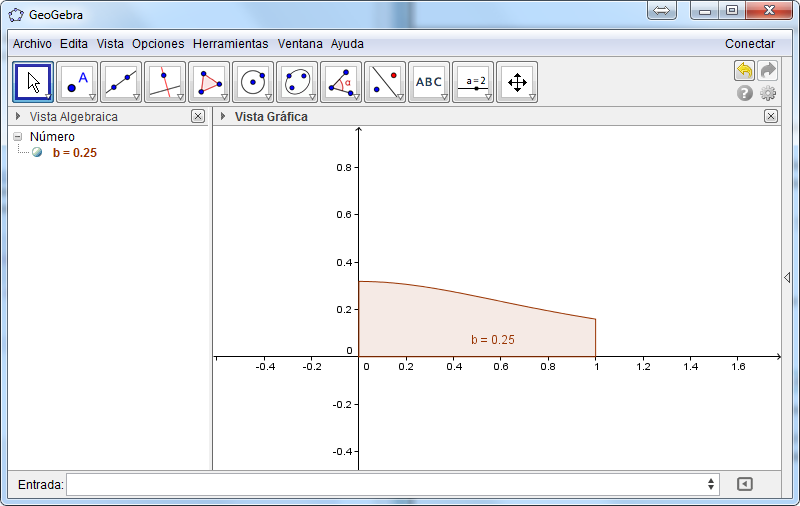
\includegraphics[width=15cm]{../fig/Tut05-49.png}
\end{center}
Aunque también aparece a la izquierda, en la {\em Vista Algebraica}. Y si lo escribes en el panel de Cálculo Simbólico obtendrás una respuesta simbólica. ¡Pruébalo!

Continuando con esta misma variable aleatoria continuas, en el Ejemplo \ref{curso-cap05:ejem:DistribucionCauchyTrucosProbabilidad} del libro (pág. \pageref{curso-cap05:ejem:DistribucionCauchyTrucosProbabilidad}) hemos usado la primitiva de esta función para comprobar que la probabilidad
    \[
    P(X \geq 1)=\int_1^{\infty}f(x)dx=\int_0^1\dfrac{1}{\pi(1+x^2)}dx,
    \]
es igual a $\frac{1}{4}$. Vamos a usar GeoGebra para calcular directamente esa integral. La cuenta es muy parecida a la anterior, pero el comando ahora es:
\begin{center}
\verb#Integral[1 / (pi * (1 + x^2)), 1, #$\infty${\tt ]}
\end{center}
Si quieres teclear directamente este comando, necesitarás el símbolo de infinito.  Para obtenerlo, puedes usar la paleta de símbolos de GeoGebra, que aparece al hacer clic sobre el icono $\begin{array}{l}
\includegraphics[width=0.5cm]{../fig/Tut05-50.png}\end{array}$ situado a la derecha de la {\em Línea de Entrada}.
\begin{center}
    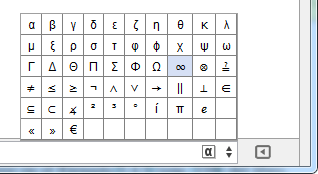
\includegraphics[width=5cm]{../fig/Tut05-51.png}
\end{center}

\begin{ejercicio}
\label{tut05:ejercicio13}
\quad\\
\begin{enumerate}
  \item Repite el cálculo de las integrales
    \[
        \int_0^1\dfrac{1}{\pi(1+x^2)}dx,
    \]
    y
    \[
        \int_1^{\infty}\dfrac{1}{\pi(1+x^2)}dx,
    \]
    con Wolfram Alpha y Wiris.

  \item Calcula, usando Wiris, el valor de la integral
    \[
    \int_{\frac{1}{2}}^{\frac{3}{4}} 6\cdot(x-x^2) dx
    \]
    que aparece en el Ejemplo \ref{curso-cap05:ejem:FuncionDensidadSoporteFinito} (pág. \pageref{curso-cap05:ejem:FuncionDensidadSoporteFinito}) del libro.

  \item Calcula, también con Wiris, una primitiva (o integral indefinida) de la función $f(x)=6\cdot(x-x^2)$.

  \item Comprueba, usando GeoGebra, que $f(x)=6\cdot(x-x^2)$, con soporte en el intervalo $0\leq x\leq 1$ (la función vale $0$ fuera de ese intervalo) es una función de densidad. Es decir, comprueba que:
    \[
    \int_{0}^{1} 6\cdot(x-x^2) dx = 1
    \]

  \item Repite el apartado anterior con Wolfram Alpha o Wiris.

  %\item Vamos a usar GeoGebra para comprobar el resultado del Ejemplo \ref{curso-cap05:ejem:DistribucionCauchyIntegralTotal1}. Es decir, vamos a comprobar que se cumple:
%      \[\int_{-\infty}^{\infty}\dfrac{1}{\pi(1+x^2)}dx = 1.\]
%      Para hacerlo, ejecuta en el panel de cálculo simbólico de GeoGebra el comando:
%        \begin{center}
%        \verb#Integral[1 / (pi * (1 + x^2)), #$-\infty, \infty${\tt ]}
%        \end{center}
%      descubrirás que para GeoGebra ese valor es {\em Indefinido} (algo así como el {\tt NaN} de R). Pero si calculas la mitad derecha de la integral:
%        \begin{center}
%        \verb#Integral[1 / (pi * (1 + x^2)), 0, #$\infty${\tt ]}
%        \end{center}
%      sorprendentemente no hay ningún problema. Compruébalo.
\end{enumerate}
Soluciones en la página \pageref{tut05:ejercicio13:sol}.
\qed
\end{ejercicio}


\subsection{Funciones definidas a trozos con GeoGebra}
\label{tut05:subsec:FuncionesDefinidasTrozosGeoGebra}

Cuando trabajamos con variables aleatorias continuas con soporte en un intervalo (ver la Sección \ref{curso-cap05:subsec:VariablesContinuasSoporteIntervalo} del libro, pág. \pageref{curso-cap05:subsec:VariablesContinuasSoporteIntervalo}), tenemos que usar funciones de densidad definidas a trozos (mediante llaves), como en la función del Ejemplo \ref{curso-cap05:ejem:FuncionDensidadSoporteFinito} de esa sección:
 \[f(x)=\begin{cases}6\cdot(x-x^2),&\mbox{ para }0\leq x\leq 1.\\ 0,&\mbox{en otro caso}.\end{cases}\]
Esta breve sección sirve sólo para hacer justicia al excelente trabajo que han hecho los programadores de las últimas versiones de GeoGebra, para que el programa sea capaz de trabajar adecuadamente con este tipo de funciones. La clave es la instrucción {\tt Si}, que permite que el resultado de una función dependa del cumplimiento de una cierta condición. Por ejemplo, para definir en GeoGebra la anterior función $f$ basta con teclear, en la {\em Línea de Entrada} de GeoGebra, el siguiente comando:
\begin{center}
    \verb#f(x) = Si[0 < x < 1, 6*(x - x^2), 0]#
\end{center}
El resultado se muestra en esta figura:
    \begin{center}
        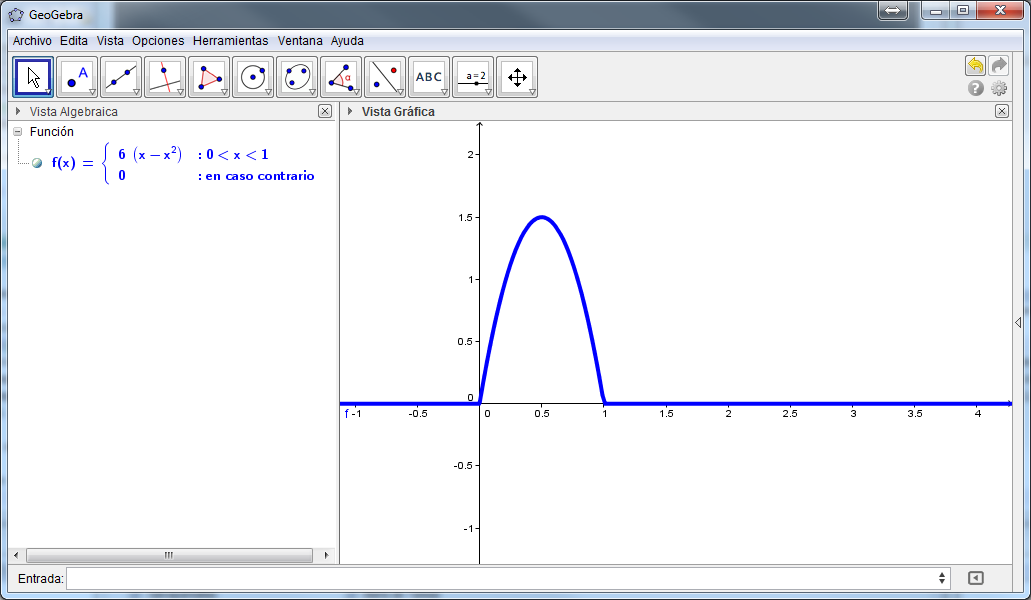
\includegraphics[width=14cm]{../fig/Tut05-57.png}
    \end{center}
Hemos coloreado de azul la gráfica para que veas que la función está definida para todos los valores de $x$, no sólo para los del intervalo $[0,1]$. Fíjate también en que la descripción de la función que hace GeoGebra en el panel de {\em Vista Algebraica} (a la izquierda) es impecable. Realmente los programadores han hecho un gran trabajo. Que se traduce, entre otras cosas, en que el cálculo de probabilidades para esta variable se puede realizar de forma muy cómoda. Si, por ejemplo, queremos calcular
\[P\left( \dfrac{3}{7} < X < \dfrac{23}{15}\right)\]
podemos traducir directamente los extremos del intervalo a límites de integración, escribiendo:
   \begin{center}
    \verb#Integral[f(x), 3/7, 23/15]#
   \end{center}
sin preocuparnos de si esos extremos caen dentro del intervalo $[0, 1]$, o no.

\begin{ejercicio}
\label{tut05:ejercicio14}
\begin{enumerate}
  \item[]
  \item Usa ese comando en GeoGebra para calcular la probabilidad $P\left( \dfrac{3}{7} < X < \dfrac{23}{15}\right)$.
  \item Calcula la probabilidad $P(-4, 0.7)$ para la misma variable aleatoria $X$.
  \item Este ejercicio es un poco más complicado.  Supongamos que ahora $Y$ es una variable aleatoria continua, con soporte en el intervalo $[1,4]$, dada por esta función de densidad:
      \[
      g(x) = \begin{cases}
      \dfrac{2(x-1)}{3}& \mbox{ si }\quad 1\leq x < 2\\[3mm]
      \dfrac{4-x}{3}& \mbox{ si }\quad 2\leq x < 4\\[3mm]
      0&\mbox{ en cualquier otro caso.}
      \end{cases}
      \]
      Empieza por comprobar que $g(x)$ es realmente una función de densidad. Una vez hecho esto, calcula la probabilidad:
      \[P\left(\dfrac{1879}{1250} < Y < \dfrac{2511}{625}\right).\]
\end{enumerate}
Solución en la página \pageref{tut05:ejercicio14:sol}.\qed
\end{ejercicio}


\subsection{Media y varianza de variables aleatorias continuas.}
\label{tut05:subsec:MediaVarianzaVariablesAleatoriasContinuas}

Si hemos conseguido perderle el miedo a las integrales, las fórmulas para el cálculo de medias y varianzas son muy fáciles de usar. En el Ejemplo \ref{curso-cap05:ejem:MediaVarianzaVariableAleatoriaContinua} del libro (pág. \pageref{curso-cap05:ejem:MediaVarianzaVariableAleatoriaContinua}) hemos calculado la media y varianza de una variable aleatoria mediante las integrales:
    \[
    \mu=\int_{1}^{2}  x f(x)dx=\int_{1}^{2}x\cdot 2\cdot(2-x)dx=\dfrac{4}{3}\approx 1.33 \]
y
    \[
    \sigma^2=
    \int_{1}^{2}(x-\mu)^2f(x)dx =
    2\int_{1}^{2}\left(x-\dfrac{4}{3}\right)^2(2-x)dx=\dfrac{1}{18}\approx 0.05556
    \]
respectivamente. Comprobar estos resultados, con cualquiera de los programas que venimos utilizando, es muy sencillo. Por ejemplo, para calcular la media usando GeoGebra basta con ejecutar estos comandos, uno tras otro:
\begin{center}
\begin{tabular}{ll}
    &\verb#f(x) = 2 * (2 - x)#\\
    &\verb#mu = Integral[ x * f(x), 1, 2]#\\
    &\verb#sigma = Integral[ (x - mu)^2 * f(x), 1, 2]#
\end{tabular}
\end{center}
Como de costumbre en GeoGebra se muestran los resultados numéricos, no simbólicos. Usa la opción {\em Redondeo} del menú {\em Opciones}, si deseas ver más cifras significativas.

\begin{ejercicio}
\label{tut05:ejercicio15}
\begin{enumerate}
  \item[]
  \item Repite estas integrales con Wiris y Wolfram Alpha.

  \item Calcula la media y varianza de la función del Ejemplo \ref{curso-cap05:ejem:FuncionDensidadSoporteFinito} del libro (pág. \pageref{curso-cap05:ejem:FuncionDensidadSoporteFinito}), que ya hemos usado antes en este tutorial, al principio de la Sección \ref{tut05:subsec:FuncionesDefinidasTrozosGeoGebra} (pág. \pageref{tut05:subsec:FuncionesDefinidasTrozosGeoGebra}).

  \item
   Hemos empezado nuestro trabajo sobre variables aleatorias continuas hablando de la función de densidad
  \[f(x)=\dfrac{1}{\pi(1+x^2),}\]
  que define la que se conoce como {\em distribución de Cauchy}. Y dijimos que era una función simple, pero no engañosamente simple. Para entender en qué sentido este ejemplo no es trivial del todo, trata de calcular su media, con cualquiera de los programas que hemos usado. Comprobarás que {\em la media no existe}, porque la integral
  \[\int_{-\infty}^{\infty} x\cdot \dfrac{1}{\pi(1+x^2)} dx\]
  es una {\em indeterminación de la forma $\infty - \infty$}. En concreto, la integral se puede escribir como una suma:
  \[\int_{-\infty}^{0} x\cdot \dfrac{1}{\pi(1+x^2)} dx + \int_{0}^{\infty} x\cdot \dfrac{1}{\pi(1+x^2)} dx,\]
  en la que la primera integral vale $-\infty$ y la segunda vale $\infty$. Usa el ordenador para comprobar esto.
\end{enumerate}
Soluciones en la página \pageref{tut05:ejercicio15:sol}.
\qed
\end{ejercicio}

\paragraph{Observaciones sobre el último apartado de este ejercicio:}
\label{tut05:parag:IntegralMediaCauchyNoConverge}
El resultado del último apartado plantea algunas dificultades teóricas. No te preocupes demasiado si no lo entiendes del todo la primera vez que lo leas. Es una buena idea usar GeoGebra o Wolfram Alpha para dibujar la gráfica de
\[h(x) = x\cdot \dfrac{1}{\pi(1+x^2)},\]
como hemos hecho nosotros en la siguiente figura. La simetría de las dos mitades de esa gráfica ayuda a entender porque el resultado de las dos integrales es el mismo, pero con signos opuestos. Y el área de la mitad derecha, la zona sombreada de la figura, es igual a $\infty$. Un matemático diría que la integral de $0$ a $\infty$ es {\sf divergente}.
\begin{center}
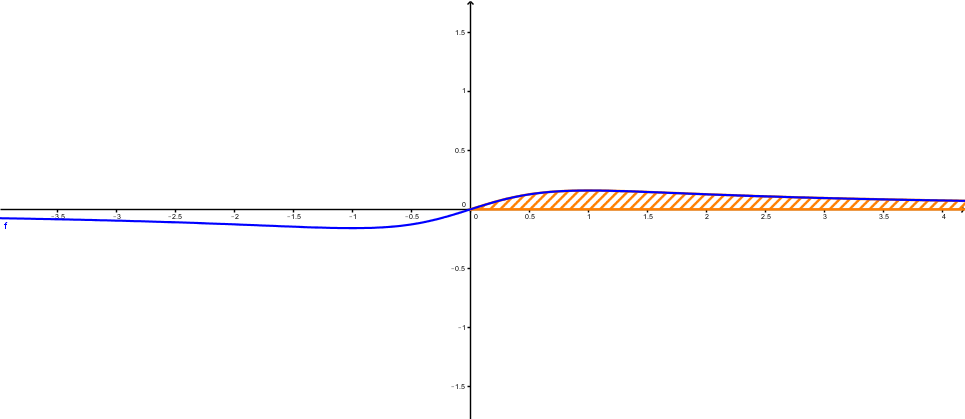
\includegraphics[width=14cm]{../fig/Tut05-69.png}
\end{center}
¿Por qué es divergente esta integral? Es decir, ¿por qué ese área es igual a $\infty$? Si miras la figura verás que la {\em base} de la figura es el intervalo $(0, +\infty)$, mientras que la altura, dada por la función $h(x)$, se hace más y más pequeña (tiende a $0$) a medida que $x$ aumenta. Si piensas en una fórmula del tipo ``base $\cdot$ altura'', lo que sucede aquí es que la base tiende a $\infty$, mientras la altura tiende a $0$. Así que el área es $\infty \cdot 0$, una indeterminación. Las indeterminaciones, en las que dos cantidades exhiben comportamientos enfrentados, se resuelven en Matemáticas estudiando la {\em velocidad} relativa a la que se mueven esas cantidades. Pero medir esas velocidades y detectar las diferencias entre ellas, que a veces son sutiles, puede ser un trabajo muy complicado. En el Tutorial03 nos encontramos con una situación muy similar al hablar de {\em series} (sumas de infinitos números). Y allí ya dijimos que la clave era el análisis de la velocidad a la que cambiaban las cantidades involucradas. A menudo, para resolver el problema satisfactoriamente se hace necesario consultar con un experto, un matemático. Una consecuencia importante de esas dificultades teóricas es que los programas de ordenador a veces se ven en un aprieto para calcular este tipo de integrales. En el menos malo de los casos,  el programa nos dirá algo así como ``no sé calcular esta integral'', y al menos sabremos que tenemos un problema. Pero en ocasiones, las decisiones que hay que tomar en el cálculo de las integrales son  tan complicadas que los programas fallan, y producen un resultado erróneo. Veremos un ejemplo en la Sección

¿Qué consecuencias tiene el hecho de que no exista la media? Todavía no podemos contestar con propiedad a esta pregunta, hasta que no hayamos discutido algo sobre distribuciones muestrales en el Capítulo \ref{curso-cap:IntervalosConfianza} del libro. Pero te podemos adelantar algo: la media se ha diseñado para ser un {\em ``buen representante''} de un conjunto de datos. Si no existe la media, quiere decir que, por alguna razón, no es posible elegir un buen representante para esos datos. Y, a otro nivel, si no existe la media desde luego tampoco existe la varianza.


\subsection{La variable de integración.}
\label{tut05:subsection:VariableIntegracion}

Más adelante, en la Sección \ref{curso-cap05:subsec:DistribucionUniforme} (pág. \pageref{curso-cap05:subsec:DistribucionUniforme}) del libro, hemos necesitado calcular una primitiva de la función
\[
f(x)=\begin{cases}
k&\mbox{ si }a<x<b\\
0&\mbox{ en otro caso. }
\end{cases}
\]
donde $k$ es una constante. Nuestro objetivo aquí es encontrar cuál es el valor de $k$ que hace que esta función sea una función de densidad y, para eso, se necesita que su integral en el intervalo $[a,b]$ sea igual a 1.

La dificultad es que, si usamos un programa como GeoGebra, Wiris o Wolfram Alpha para calcular esa primitiva, tenemos que asegurarnos de que el programa entiende que la variable de la función es $x$ y no $k$. Nosotros sabemos que queremos pensar en $x$ como una variable y $k$ como una constante, pero si no le proporcionamos más información, entonces para el programa $x$ y $k$ son dos símbolos cualesquiera, y puede interpretar ambos como variables.

\subsubsection*{Wiris.}

En Wiris basta, en principio, con ser cuidadosos. Debemos usar el símbolo de integral que incluye el diferencial (la d final, y  colocar la variable de integración en ese símbolo de diferencial.

Quizá la mejor manera de entenderlo sea con un ejemplo. En la siguiente figura puedes ver el cálculo de una primitiva de $k$, hecho de tres maneras con Wiris, que hemos numerado (en rojo) para discutirlas.
\begin{center}
    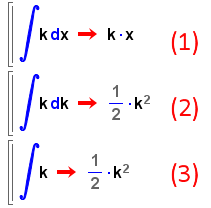
\includegraphics[width=5cm]{../fig/Tut05-18.png}
\end{center}
\begin{enumerate}
  \item La primera, que es la que necesitamos en este caso, usa el diferencial $dx$, y en ese caso Wiris interpreta correctamente $k$ como una constante. La primitiva es $F(x)=k\cdot x$.
  \item En la segunda, para ilustrar el problema, hemos usado el diferencial $dk$. Esto hace que Wiris interprete $k$ como una variable, y la primitiva resultante es $\dfrac{k^2}{2}$. Si usáramos esto cometeríamos un error. Insistimos: para nosotros $k$ es una constante.
  \item En el paso anterior, es posible que el lector piense que es un error difícil de cometer, porque tenemos que colocar ex profeso la $k$ en el diferencial. Esta última versión ilustra la forma en que, habitualmente, se comete ese error. Aquí usamos el símbolo de integral sin diferencial, y en ese caso Wiris tiene que decidir, por si mismo, cual es la variable. Y como sólo aparece la $k$, Wiris elige esta como variable.
\end{enumerate}
En conclusión, es conveniente que, en Wiris, utilices siempre la integración con diferenciales, y escribas explícitamente la variable con respecto a la que integras.

\subsubsection*{Wolfram Alpha.}

¿Qué sucede en Wolfram Alpha? Algo muy parecido:
\begin{enumerate}
  \item Cuando escribimos {\tt integrate(k, x)}, indicándole a Wolfram Alpha que la variable de integración es $x$, obtenemos la respuesta correcta:
      \[\int k dx= k\cdot x+\mbox{constant}\]
      (Y recuerda que puedes tomar la constante {\tt constant} igual a 0).

  \item Si escribimos {\tt integrate(k, k)}, señalando a $k$ como variable de integración es $x$, obtenemos una respuesta que, en este caos, es un error:
      \[\int k dk= \dfrac{k^2}{2}+\mbox{constant}\]

  \item Y por último, y más peligroso, si escribimos {\tt integrate(k)}, y dejamos que sea el programa quien decida, obtenemos de nuevo la respuesta errónea.
\end{enumerate}

\subsubsection*{GeoGebra.}

En GeoGebra hemos empezado por abrir el panel de {\em Cálculo Simbólico}, y hemos tecleado el comando
\begin{center}
  \verb#f(x) := k#
\end{center}
El símbolo {\tt :=} es la forma de asignar valores a símbolos en este panel de {\em Cálculo Simbólico}. Una vez hecho esto (y tras pulsar {\tt Entrar}, claro), basta con ejecutar el comando
\begin{center}
  \verb#Integral[f(x), x]#
\end{center}
en el que, como en los otros casos, hemos tenido que indicar la variable de integración.

\begin{ejercicio}
\label{tut05:ejercicio16}
\quad\\
En todos los casos, es conveniente que intentes hacer los ejercicios usando varios de los programas, para cotejar los resultados.
\begin{enumerate}
  \item En el ejemplo que acabamos de describir con GeoGebra, ejecuta uno tras otro, para comparar los resultados, los comandos
  \begin{center}
  \begin{tabular}{l}
  {\tt Integral[f(x), k]}\\
  {\tt Integral[f(x)]}
  \end{tabular}
  \end{center}
  \item Calcula una primitiva de $f(x)=x\cdot\cos(3x)$
  \item Calcula el valor de $k$ para que la función:
    \[
        f(x)=\begin{cases}
        k\cdot x\cdot\cos(3x)&\mbox{ si }0<x<\dfrac{\pi}{6}\\
        0&\mbox{ en otro caso. }
        \end{cases}
    \]
    sea una función de densidad en el intervalo $0\leq x\leq\dfrac{\pi}{6}$.
  \item Utiliza el ordenador para comprobar las integrales intermedias del Ejemplo \ref{curso-cap05:ejem:FuncionDistribucionVariableContinua} del libro (pág. \pageref{curso-cap05:ejem:FuncionDistribucionVariableContinua}) y también las del Ejemplo \ref{curso-cap05:ejem:FuncionDistribucionDensidadSoporteIntervalos} (pág. \pageref{curso-cap05:ejem:FuncionDistribucionDensidadSoporteIntervalos}).
  \item Usa Wolfram Alpha, GeoGebra o Wiris para resolver la ecuación cuadrática
        \[-\dfrac{2 k^2}{3}+4 k-5=\dfrac{1}{2}.\]
        que aparece en el Ejemplo \ref{curso-cap05:ejem:FuncionDistribucionDensidadSoporteIntervalos}.
\end{enumerate}
Soluciones en la página \pageref{tut05:ejercicio16:sol}.
\qed
\end{ejercicio}

\subsection{La distribución uniforme con R.}
\label{tut05:subsubsec:DistribucionUniformeR}

En la Sección \ref{curso-cap05:subsec:DistribucionUniforme} del libro (pág. \pageref{curso-cap05:subsec:DistribucionUniforme}) hemos hablado de las distribuciones uniformes. Una distribución uniforme definida en el intervalo $[a,b]$ tiene soporte en dicho intervalo (es decir, su densidad vale $0$ fuera del intervalo) y es constantemente igual a $1/(b-a)$ dentro del intervalo. R nos ofrece varias herramientas para trabajar con densidades uniformes. En concreto, vamos a hablar de las funciones:
\begin{center}
  {\tt punif,\qquad dunif,\qquad qunif,\qquad runif.}
\end{center}
Como ves, el sufijo común a todas ellas es {\tt unif}. La primera de ellas, {\tt pbinom}, proporciona la respuesta a la pregunta:
\[P(X \leq k)\]
siendo $X$ una variable uniforme en el intervalo $[a,b]$. Por ejemplo, si $X$ es una variable uniforme definida en el intervalo $[5,13]$, y queremos saber cual es la probabilidad
\[P(X \leq 11)\]
ejecutaremos en R el siguiente código:
\begin{knitrout}
\definecolor{shadecolor}{rgb}{0.969, 0.969, 0.969}\color{fgcolor}\begin{kframe}
\begin{alltt}
\hlkwd{punif}\hlstd{(}\hlnum{11}\hlstd{,} \hlkwc{min} \hlstd{=} \hlnum{5}\hlstd{,} \hlkwc{max} \hlstd{=} \hlnum{13}\hlstd{)}
\end{alltt}
\begin{verbatim}
## [1] 0.75
\end{verbatim}
\end{kframe}
\end{knitrout}
Como ves, las opciones {\tt min} y {\tt max} nos permiten indicarle a R cuál es el intervalo $[a, b]$ en el que se define la distribución uniforme. La función {\tt punif} es, por tanto, la función de distribución de la variable $X$. Y, por tanto, si queremos calcular la probabilidad de un subintervalo, como en
\[P(8\leq X \leq 11)\]
basta con tomar la diferencia de los valores de {\tt punif} al final y al principio de ese subintervalo:
\begin{knitrout}
\definecolor{shadecolor}{rgb}{0.969, 0.969, 0.969}\color{fgcolor}\begin{kframe}
\begin{alltt}
\hlkwd{punif}\hlstd{(}\hlnum{11}\hlstd{,} \hlkwc{min} \hlstd{=} \hlnum{5}\hlstd{,} \hlkwc{max} \hlstd{=} \hlnum{13}\hlstd{)} \hlopt{-} \hlkwd{punif}\hlstd{(}\hlnum{8}\hlstd{,} \hlkwc{min} \hlstd{=} \hlnum{5}\hlstd{,} \hlkwc{max} \hlstd{=} \hlnum{13}\hlstd{)}
\end{alltt}
\begin{verbatim}
## [1] 0.375
\end{verbatim}
\begin{alltt}
\hlstd{(}\hlnum{11} \hlopt{-} \hlnum{8}\hlstd{)} \hlopt{/} \hlstd{(}\hlnum{13} \hlopt{-} \hlnum{5}\hlstd{)}
\end{alltt}
\begin{verbatim}
## [1] 0.375
\end{verbatim}
\end{kframe}
\end{knitrout}
Hemos incluido él cálculo de esa probabilidad mediante la Ecuación \ref{curso-cap05:ecu:ProbabilidadSubintervaloUniforme} del libro (pág. \pageref{curso-cap05:ecu:ProbabilidadSubintervaloUniforme}), para que veas que los resultados coinciden.

Cuando vimos las funciones de R para trabajar con la binomial, hablamos de {\tt dbinom} antes de hablar de {\tt pbinom}. Ahora hemos empezado hablando de {\tt punif}. ¿Qué sucede con {\tt dunif}?

    \begin{center}
    \fcolorbox{black}{Gris025}{
    \begin{minipage}{12cm}
    \begin{center}
      {\bf Densidad de variables aleatorias continuas en R.\\ Funciones que empiezan por {\tt d}.}
    \end{center}
    Los cálculos de probabilidad, en una distribución uniforme, {\bf siempre} se llevan a cabo con {\tt punif}. Al tratarse de una distribución continua, la función {\tt dunif} representa la densidad de probabilidad, y {\bf no es una probabilidad} (hay que integrarla para obtener la probabilidad). En particular, cuando se trata de distribuciones continuas, prácticamente nunca vamos a usar las funciones de R que empiezan por {\tt d}.
    \end{minipage}
    }
    \end{center}

Para insistir en estas ideas vamos a hacer un ejercicio.
\begin{ejercicio}
\label{tut05:ejercicio17}
\quad\\
Vamos a definir una variable aleatoria uniforme en el intervalo $\left[\dfrac{1}{130}, \dfrac{12}{130}\right]$. Calcula las probabilidades:
\begin{enumerate}
  \item $P\left(X < \dfrac{6}{130}\right)$.
  \item $P\left(\dfrac{2}{130} < X < \dfrac{9}{130}\right)$.
  \item Repite los cálculos anteriores cambiando $<$ por $\leq$. ¿Hay alguna diferencia? ¿Por qué sucede esto?
  \item Calcula {\tt dunif(6/130, min=1/130, max=12/130)}. ¿Puede ser ese valor una probabilidad? Calcula también {\tt dunif(20/130, min=1/130, max=12/130)}. Fíjate en que el valor $\frac{20}{130}$ está fuera del intervalo soporte de esta función uniforme.
  \item Calcula la probabilidad $P(X > 6/130)$ (y también con $\geq$ en lugar de $>$).
\end{enumerate}
Soluciones en la página \pageref{tut05:ejercicio17:sol}.
\qed
\end{ejercicio}
Como hemos dicho ya antes, R utiliza siempre por defecto probabilidades de la forma $P(X \leq k)$. Si quieres que use desigualdades de la forma $P(X < k)$ puedes usar la opción {\tt lower.tail= FALSE}.

La función {\tt qunif} permite responder a esta pregunta: dada la probabilidad $p_0$, ¿cuál es el valor $k$ para el que $P(X\leq k) = p_0$? Es decir, ¿cuál es el cuantil $p_0$ de $X$? Por ejemplo, si $X$ es una distribución uniforme en el intervalo $[-11, 25]$ y queremos calcular su cuantil $0.75$ (el tercer cuartil), usaríamos este comando:
\begin{knitrout}
\definecolor{shadecolor}{rgb}{0.969, 0.969, 0.969}\color{fgcolor}\begin{kframe}
\begin{alltt}
\hlkwd{qunif}\hlstd{(}\hlnum{0.75}\hlstd{,} \hlkwc{min}\hlstd{=}\hlopt{-}\hlnum{11}\hlstd{,} \hlkwc{max}\hlstd{=}\hlnum{25}\hlstd{)}
\end{alltt}
\begin{verbatim}
## [1] 16
\end{verbatim}
\end{kframe}
\end{knitrout}
Vamos a comprobar el resultado:
\begin{ejercicio}
\label{tut05:ejercicio18}
\quad\\
Guarda el resultado del anterior comando en la variable {\tt k} de R, y usa {\tt punif} para comprobar que $P(X\leq k) = 0.75$.
Solución en la página \pageref{tut05:ejercicio18:sol}.
\qed
\end{ejercicio}

Jugando con las propiedades de las probabilidades, se puede usar {\tt qunif} para responder a preguntas más generales.
\begin{ejercicio}
\label{tut05:ejercicio19}
\quad\\
Sea $X$ una variable aleatoria uniforme en el intervalo $[-2, 8]$. Calcula el valor $k$ para el que se cumple $P(X > k) = \dfrac{1}{7}$. Comprueba el resultado. Solución en la página \pageref{tut05:ejercicio19:sol}.
\qed
\end{ejercicio}

Finalmente, la función {\tt runif} sirve para obtener valores aleatorios de una variable aleatoria uniforme. Esta función es extremadamente útil a la hora de hacer simulaciones, porque sirve para poner en práctica esa idea de {``lanzar un dardo al azar dentro del intervalo $[a, b]$, de forma que todas las regiones del intervalo sean igual de probables''.} Vamos a usar un ejercicio para ver cómo usar esto.

\begin{ejercicio}
\label{tut05:ejercicio20}
\quad\\
Sea $X$ una variable aleatoria uniforme en el intervalo $[-5, 5]$.
\begin{enumerate}
  \item Usa {\tt runif} para generar un vector de $n=1000$ puntos aleatorios dentro de ese intervalo. Llama {\tt puntos} a ese vector.
  \item Calcula, con {\tt punif}, la probabilidad de que uno de esos puntos pertenezca al intervalo $[-1, 3]$.
  \item ¿Qué {\em fracción} (o porcentaje) de los elementos de {\tt puntos} pertenecen de hecho al intervalo $[-1, 3]$?
  \item Repite los apartados anteriores para $n = 10000$ y $n = 1000000$.
  \item {\bf Más difícil:} En lugar de GeoGebra, se puede usar R para simular el lanzamiento de dardos dentro de un cuadrado de lado $4$, y calcular el valor de $\pi$, como hemos hecho en el Ejemplo \ref{curso-Cap03:ejem:ProbabilidadGeometricaMontecarlo} del libro (pág. \pageref{curso-Cap03:ejem:ProbabilidadGeometricaMontecarlo}). Puedes hacer esto así:
      \begin{enumerate}
        \item Construyes $n$ valores de $x$ uniformemente distribuidos en el intervalo $[-2, 2]$.
        \item De la misma forma, construyes $n$ valores de $y$ uniformemente distribuidos en el intervalo $[-2, 2]$. Estos valores de $y$ son, desde luego, independientes de los de $x$.
        \item Al emparejar cada  valor de  $x$ con el correspondiente valor de $y$ el punto $(x, y)$ resultante es un punto al azar en el cuadrado de lado $4$ centrado en el origen.
        \item Para saber si un punto de coordenadas $(x,y)$ ha caído en el interior del círculo de radio $1$, basta con ver si se cumple la condición
        \[x^2 + y^2 < 1.\]
        \item Una vez que sepas la fracción de puntos que han caído en el círculo, multiplica esa fracción por $16$ (el área del cuadrado), para estimar qué fracción del área del cuadrado corresponde al área del círculo de radio $1$. Eso te permitirá obtener un valor aproximado de $\pi$.
      \end{enumerate}
      La ventaja de R, frente a GeoGebra, es que R puede usar un número enorme de puntos sin problemas. Usa este esquema, y un número muy grande de puntos (del orden de millones) para estimar el valor de $\pi$. En el código de la solución veremos, además, las instrucciones necesarias para dibujar cada uno de los pasos anteriores.
\end{enumerate}
Soluciones en la página \pageref{tut05:ejercicio20:sol}.
\qed
\end{ejercicio}



\section{La distribución normal.}
\label{tut05:sec:DistribucionNormal}

En esta sección nos vamos a ocupar de la más importante de todas las distribuciones continuas, la normal. Veremos cómo usar los programas de ordenador que conocemos (GeoGebra, Wolfram Alpha y, desde luego, R) para trabajar con variables aleatorias de tipo normal.

\subsection{La familia de las curvas normales con GeoGebra.}

Para empezar a familiarizarnos con las distribuciones normales, vamos a comenzar conociendo las herramientas que GeoGebra nos brinda para trabajar con este tipo de distribuciones. En primer lugar, vamos a volver a abrir la {\em Calculadora de Probabilidades} que ya conocimos al tratar con la distribución binomial en la Sección \ref{tut05:sec:DistribucionBinomial} de este Tutorial. Al abrirla, GeoGebra nos muestra precisamente la distribución normal.

\begin{center}
    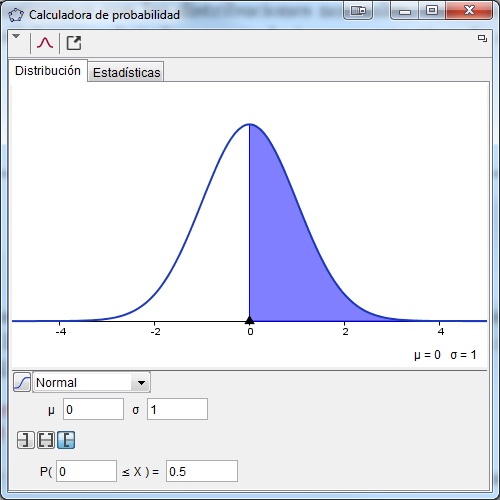
\includegraphics[width=9cm]{../fig/Tut05-59.png}
\end{center}

Para ver cómo usar la {\em Calculadora de Probabilidades}, vamos a considerar una variable aleatoria $X$ de tipo $N(3, 0.7)$ (esto es, con media $\mu = 3$ y desviación típica $\sigma = 0.7$) y vamos a calcular la probabilidad:
\[P( 1.6 < X < 4.4)\]
Para hacerlo, introduce los valores de $\mu$ y $\sigma$ en los campos adecuados de la {\em Calculadora de Probabilidades}. Después, y puesto que se trata de un intervalo, haz clic con el ratón en el icono central del grupo de iconos
\begin{center}

\includegraphics[width=2cm]{../fig/Tut05-26.png}
\end{center}
que ya discutimos al hablar de la binomial. Al seleccionar ese icono la parte inferior de la {\em Calculadora de Probabilidades} cambia para adaptarse al tipo de pregunta que queremos formular. Asegúrate de introducir los extremos del intervalo $1.6$ y $4.4$ en los campos adecuados, para que la ventana de la {\em Calculadora de Probabilidades} tenga este aspecto:
\begin{center}
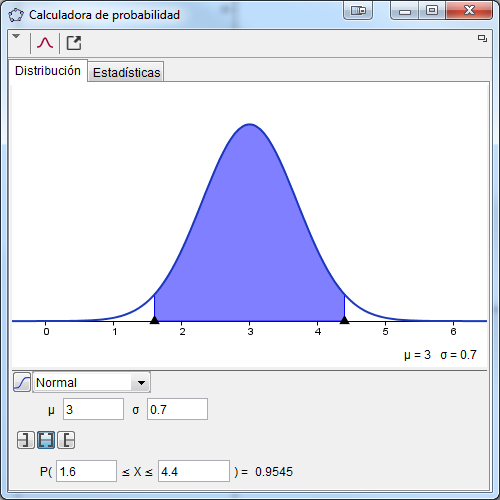
\includegraphics[width=9cm]{../fig/Tut05-60.png}
\end{center}
Como ves, la probabilidad que buscábamos es, aproximadamente, $0.9545$. La solución, además, se ilustra gráficamente. La {\em Calculadora de Probabilidades} también se puede utilizar para calcular cuantiles. Por ejemplo, en esa misma variable de tipo $N(3, 0.7)$ vamos a buscar el valor $k$ tal que:
\[P( X \leq k) = 0.60\]
Es decir, el percentil $60$ de esta variable. Para ello, selecciona el icono izquierdo del grupo $\begin{array}{c}
\includegraphics[width=1.5cm]{../fig/Tut05-26.png}\end{array}$, y teclea $0.60$ en el campo situado a la derecha del {\tt =}, como se ve en la Figura.
\begin{center}
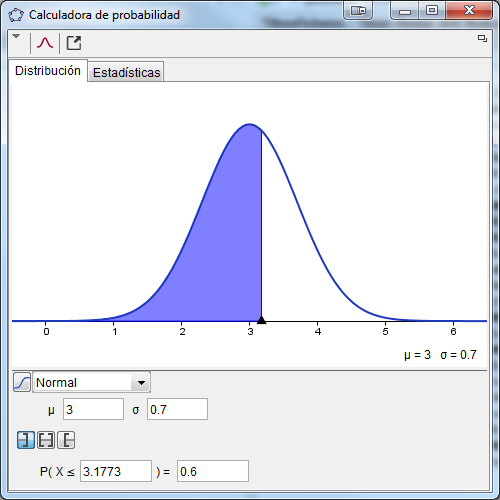
\includegraphics[width=9cm]{../fig/Tut05-61.png}
\end{center}
Tras pulsar {\tt Entrar}, GeoGebra te mostrará (dentro del símbolo de probabilidad) que el valor de $k$ es, aproximadamente, $3.1773$ (y, de nuevo, la solución se ilustra gráficamente). Fíjate en que, al ser $0.6$ ligeramente mayor que $1/2$, la probabilidad incluye toda la mitad izquierda del área bajo la curva, y una pequeña parte de la mitad derecha del área. Es una buena idea acostumbrarse a pensar geométricamente en las probabilidades que estamos calculando, tratando siempre de traducirlas en términos de áreas. Vamos a proponerte una serie de ejercicios relacionados con el cálculo de probabilidades en las distribuciones normales. Es un tipo de ejercicios que nos resultará muy útil más adelante. Insistimos en que trates de buscar siempre el sentido geométrico de estos cálculos.

\begin{ejercicio}
\label{tut05:ejercicio21}
\quad\\
En los siguientes ejercicios sea $X$ una variable aleatoria de tipo $N(5, 3)$. Calcula las probabilidades y valores que se indican.
\begin{enumerate}
  \item $P(X > 6)$, $P(X > 7)$ y, finalmente, $P(X > 10)$. ¿Qué observas?
  \item $P(X < 4)$, $P(X < 3)$ y, finalmente, $P(X < 0)$. ¿Ves alguna relación con los valores del anterior apartado?
  \item $P(4.5 < x < 5.5)$, $P(2 < X < 8)$ y, finalmente, $P( 0 < X < 10)$.
  \item Los valores $k_1$ y $k_2$ tales que $P(X < k_1) = 0.90$ y $P(X < k_2) = 0.95$.
  \item Los valores $k_1$ y $k_2$ tales que $P(X > k_1) = 0.1$ y $P(X > k_2) = 0.05$. ¿Ves alguna relación con los valores del anterior apartado?
\end{enumerate}
Ahora, con la misma variable $X$, responde a estas preguntas, pero sin usar el ordenador:
\begin{enumerate}
  \setcounter{enumi}{5}
  \item El valor $P(X < 7)$ ¿es mayor o menor que $\frac{1}{2}$?
  \item El valor $P(X > 8)$ ¿es mayor o menor que $\frac{1}{2}$?
  \item ¿Cuál de estos dos valores es más grande, $P(X > 4)$ o $P(X < 5.5)$?
  \item El valor $k$ tal que $P(X > k) = 0.6$ ¿es mayor o menor que $5$?
  \item El valor $k$ tal que $P(X < k) = 0.1$ ¿es mayor o menor que $5$?
\end{enumerate}
Para la última parte, vuelve a la ventana principal de GeoGebra, ve al menú {\em Opciones}, y en {\em Redondeo} asegúrate de seleccionar $5$ cifras decimales.
\begin{enumerate}
  \setcounter{enumi}{10}
  \item Para comprobar los resultados del Ejemplo \ref{curso-ejem:BinomialVsNormal} del libro (pág. \pageref{curso-ejem:BinomialVsNormal}), ejecuta en la {\em Línea de Entrada} de GeoGebra, uno tras otro, los tres comandos siguientes:
      \begin{center}
      \begin{tabular}{l}
        {\tt DistribuciónBinomial[100,1/3,30,false]}\\
        {\tt f(x) = Normal[100 * (1/3), sqrt(100 * (1/3) * (2/3)), x]}\\
        {\tt f(30)}
      \end{tabular}
      \end{center}
\end{enumerate}
Soluciones en la página \pageref{tut05:ejercicio21:sol}. Para el último apartado las soluciones aparecen en el Ejemplo \ref{curso-ejem:BinomialVsNormal} del libro. \qed
\end{ejercicio}

Como hicimos con la binomial, una forma de familiarizarse con las curvas normales es utilizar las capacidades dinámicas de GeoGebra para variar (mediante deslizadores) los valores de $\mu$ y $\sigma$, y ver el efecto que tienen sobre la forma y posición de la curva. Para hacer esto, abre una nueva ventana de GeoGebra y, desde la  {\em Línea de entrada}, ejecuta consecutivamente estos comandos:
\begin{center}
\begin{tabular}{l}
{\tt  mu = Deslizador[-5, 5, 0.05, 0, 200]}\\
{\tt  sigma = Deslizador[0, 2, 0.05, 0, 200]}\\
{\tt  sigma = 1}\\
{\tt Normal[mu, sigma, x]}
{\tt RazónEjes[20,3]}
\end{tabular}
\end{center}
Puedes usar los nombres {\tt mu} y {\tt sigma}, como hemos hecho nosotros, o puedes usar los símbolos $\mu$ y $\sigma$, con el panel de caracteres de GeoGebra, que aparece a la derecha de la  {\em Línea de entrada}. El comando $sigma = 1$ nos sirve para fijar el valor inicial de {\tt sigma}, y comenzar con la normal $N(0, 1)$. El comando {\tt RazónEjes[20,3]} ajusta la relación de escalas de los dos ejes para que la visualización resulte más cómoda. Tras ejecutar todos estos comandos, tu ventana de GeoGebra tendrá un aspecto similar a este:
\begin{center}
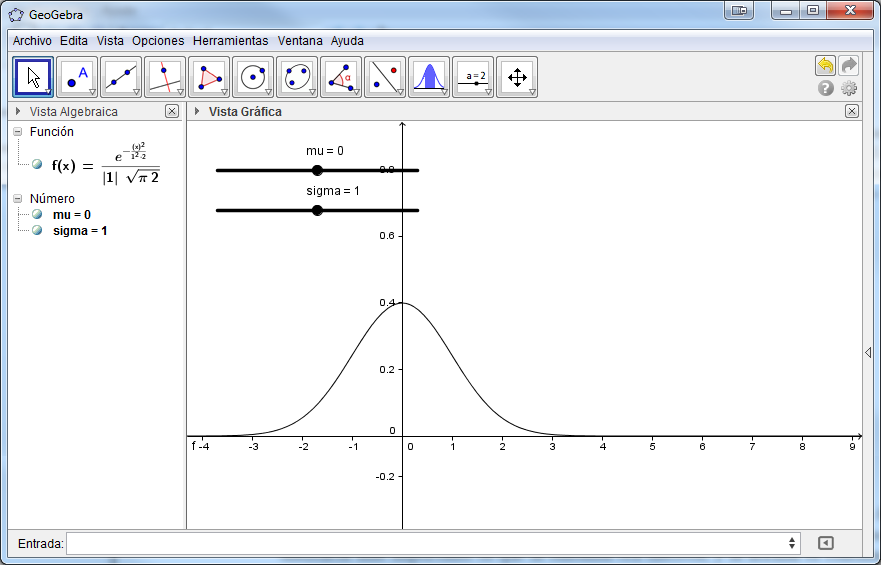
\includegraphics[width=15cm]{../fig/Tut05-63.png}
\end{center}
Fíjate en la ecuación de la curva normal, que aparece en el panel de {\em Vista Algebraica}. Ahora puedes empezar a experimentar con los deslizadores de $\mu$ y $\sigma$. ¿Qué sucede al cambiar $\mu$ o $\sigma$? ¿Cambia la forma o posición de la curva?

En cualquier caso, es importante que recuerdes que, por mucho que cambien la forma o la posición de la curva, el area total bajo esa curva siempre es igual a $1$. Para insistir en esta idea, y en cómo se distribuye la probabilidad con las curvas normales, te hemos preparado otro fichero GeoGebra, muy parecido a lo que acabamos de ver:
\begin{center}
  \fichero{../ggb/Tut05-CurvasNormalesAreas.ggb}{Tut05-CurvasNormalesAreas.ggb}
\end{center}
pero en el que puedes hacer clic en la casilla rotulada {\em ``Muestra áreas''}, para ver en acción lo que se conoce como {\em Regla 68-95-99 para las distribuciones normales} (ver Ecuación \ref{curso-cap05:ecu:Regla68-95-99Normales} en el libro, pág. \pageref{curso-cap05:ecu:Regla68-95-99Normales})

\subsection{Tratando de calcular una primitiva de la curva normal.}

En la discusión de la página \pageref{curso-cap05:ecu:IntegralNormalIntervalo} del libro hemos dicho que no es posible encontrar una primitiva de la curva normal. En un intento de hacer esta idea más cercana (ya que es bastante abstracta, a nuestro juicio), vamos a ver lo que sucede cuando le pedimos a un programa de ordenador que trate de calcular esa primitiva. En concreto, para simplificar pero sin merma de generalidad, vamos a quedarnos en el caso de la normal $N(0, 1)$, que es la que tiene la ecuación más sencilla de todas (Ecuación \ref{curso-cap05:ecu:FuncionDensidadZ} del libro, pág. \pageref{curso-cap05:ecu:FuncionDensidadZ}):
\[
f_{0,1}(x)=\displaystyle\dfrac{1}{\sqrt{2\pi}}e^{-\frac{x^2}{2}}
\]
Tratemos de calcular una primitiva usando Wiris. La siguiente figura muestra el resultado, y la flecha roja señala el mensaje con el que Wiris nos avisa de la dificultad con la que hemos tropezado.
\begin{center}
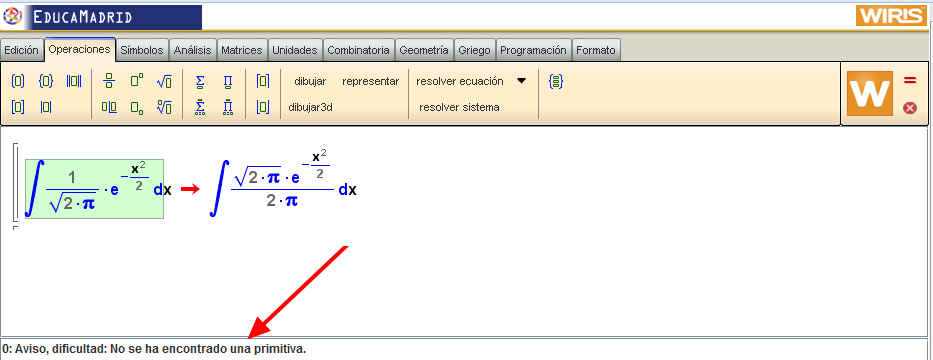
\includegraphics[width=15cm]{../fig/Tut05-65.png}
\end{center}

En Wolfram Alpha sucede algo ligeramente distinto. Escribe este comando en el programa:
\begin{center}
\verb#integrate( (1 / sqrt(2 * pi )) * exp(-x^2 / 2) )#
\end{center}
y verás que, en su respuesta, Wolfram Alpha usa una función llamada {\em erf}, del inglés {\em error function}.
\begin{center}
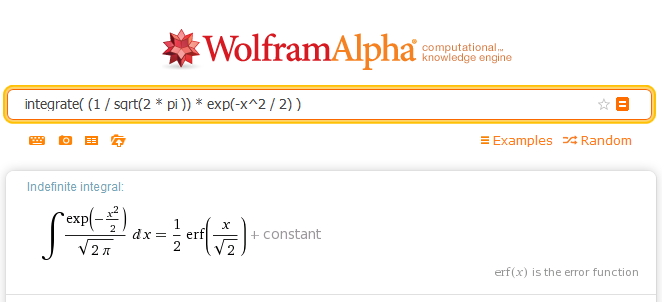
\includegraphics[width=13cm]{../fig/Tut05-64.png}
\end{center}
¿Qué es esta {\em función error erf}? Pues en el fondo, es simplemente un nombre o símbolo, que el programa utiliza para referirse a la primitiva
\[
\int e^{- x^2}dx
\]
porque Wolfram Alpha sabe que esta función no tiene una primitiva elemental. En el fondo, lo que Wolfram Alpha ha hecho ha sido avisarnos de que se ha dado cuenta de lo que estamos tratando de hacer, y  usar el nombre {\em erf} como abreviatura de ``una primitiva de $e^{-x^2/2}$. Es un mensaje tranquilizador, porque si necesitamos calcular valores de esa función {\em erf}, Wolfram Alpha nos los proporcionará sin dificultad. Por ejemplo, prueba a ejecutar
\begin{center}
{\tt erf(2)}
\end{center}
y el programa te responderá que ese valor es, aproximadamente, $0.9953$. No queremos ponernos demasiado profundos con este tema, pero en realidad, la función {\tt erf} es una función tan ``extraña'' como puedan serlo la función seno, o el logaritmo. El hecho es que en la formación matemática elemental nos han hablado de esas funciones, como las trigonométricas y el logaritmo, y nos hemos acostumbrado a verlas como teclas de la calculadora, etc. Además, las funciones trigonométricas tienen interpretaciones geométricas sencillas. Y por eso las llamamos elementales. Pero el coseno tiene tanto de elemental como pueda tenerlo {\em erf}. Para que el lector nos entienda, ¿cómo se calcula $\cos(0.32)$ ``a mano''? Al final, todos recurrimos a la calculadora o el ordenador para responder (salvo los ingenieros encargados de diseñar la calculadora, y los matemáticos que tienen que diseñar el método que usará la calculadora para hacer ese cálculo). Es en ese sentido en el que decimos que puedes pensar en {\em erf} como una ``nueva tecla de la calculadora'', y dejar los detalles para los matemáticos e ingenieros encargados del asunto.

Por cierto, GeoGebra, en su panel de {\em Cálculo Simbólico}, también usa la función {\em erf} para contestar, como ilustra esta figura:
\begin{center}
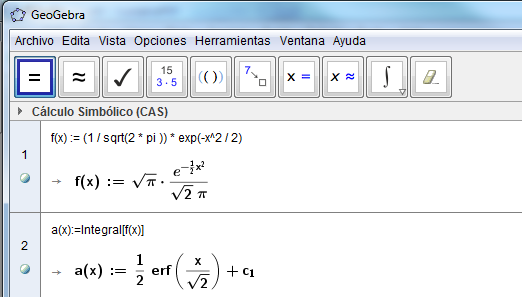
\includegraphics[width=12cm]{../fig/Tut05-66.png}
\end{center}

\section{La distribución normal en R.}
\label{tut05:subsec:DistribucionNormalR}

Al tratar con la binomial en R conocimos las funciones {\tt dbinom, pbinom, qbinom} y {\tt rbinom}. En la distribución uniforme, las correspondientes funciones fueron {\tt dunif, punif, qunif} y {\tt runif}. No es ninguna sorpresa, por tanto, que ahora, para trabajar con distribuciones normales, sea el turno de las funciones
    \begin{center}
    {\tt dnorm, \qquad     pnorm,     \qquad qnorm,  \qquad  y rnorm.}
    \end{center}
Veamos por turno el significado, y la forma de usar de cada una de estas funciones. Empezando por la primera, y de forma similar a la discusión que tuvimos en el caso de {\tt dunif}, hay que recordar que la normal es una distribución continua. Por esa razón, {\bf en este curso apenas usaremos la función {\tt dnorm}}.

%\subsection{La función {\tt dnorm}}
%\label{tut05:subsec:Dnorm}
%
%
%La función de densidad de probabilidad de una variable normal $N(\mu,\sigma)$ es
%\[f_{\mu,\sigma}(x)=\dfrac{1}{\sigma\sqrt{2\pi}} e^{-\frac{1}{2}\left(\frac{x-\mu}{\sigma}\right)^2}\]
%
%En R podemos calcular los valores de esta función mediante {\tt dnorm}. Por ejemplo, para calcular el valor de $f_{3,2}(4)$ (es decir, $\mu=3$, $\sigma=2$ y $X=4$) usaríamos un código como este:
%\begin{verbatim}
%    # Introducimos los parametros de la normal X de tipo  N(mu,sigma)
%    mu = 3
%    sigma = 2
%    # Calculamos la densidad en un valor x
%    X = 4
%    dnorm(X,mean=mu,sd=sigma)
%\end{verbatim}
%
%(y se obtiene como resultado 0.1760327).
%
%Aunque está bien saber calcular los valores de la función de densidad mediante {\tt dnorm}, lo cierto es que, tratándose de una distribución continua, no vamos a usarlos prácticamente nunca. Es muy importante recordar que
%        \begin{center}
%        \fcolorbox{black}{Gris025}{
%        \begin{minipage}{12cm}
%                        {\sf al ser la normal una distribución continua los valores de {\tt dnorm} no son probabilidades. }
%        \end{minipage}}
%        \end{center}
%De hecho, para calcular una probabilidad a partir de ellos tendríamos que integrar.
%
%%Pero, antes de despedirnos de dnorm,  vamos a aprovechar esta función para hacer una breve incursión en las capacidades gráficas de R. Para dibujar la función de densidad f, por ejemplo en el intervalo que va desde $\mu-4\sigma$ hasta  $\mu+4\sigma$, usaremos el comando curve de esta manera
%%\begin{verbatim}
%%    curve(dnorm(x,mean=mu,sd=sigma),from=mu-4*sigma,to=mu+4*sigma)
%%\end{verbatim}
%%Este es el comando curve más básico, pero podemos añadir parámetros opcionales para controlar al detalle el aspecto final del gráfico. Proponemos aquí sólo un ejemplo para que puedas experimentar cambiando los valores de algunos parámetros.
%%\begin{verbatim}
%%curve(dnorm(x,mu,sigma),from=mu-4*sigma,to=mu+4*sigma,col="red",ylim=range(0, 0.5),lwd=6)
%%\end{verbatim}

\subsection{La función {\tt pnorm}}
\label{tut05:subsec:pnorm}

Como ya hemos dicho, le vamos a dar poco o ningún uso a la función {\tt dnorm}. En cambio, la función {\tt pnorm} nos va a resultar extremadamente útil. Si tenemos una variable $X$ de tipo $N(\mu,\sigma)$ y queremos calcular el valor
\[P(X\leq k)\]
(es decir, lo que llamamos la cola izquierda de la distribución normal en el punto $k$), lo podemos hacer en R con estas instrucciones:

\begin{knitrout}
\definecolor{shadecolor}{rgb}{0.969, 0.969, 0.969}\color{fgcolor}\begin{kframe}
\begin{alltt}
\hlstd{mu} \hlkwb{=} \hlnum{3}
\hlstd{sigma} \hlkwb{=} \hlnum{2}
\hlstd{k} \hlkwb{=} \hlnum{4}
\hlkwd{pnorm}\hlstd{(k,} \hlkwc{mean}\hlstd{=mu,} \hlkwc{sd}\hlstd{=sigma)}
\end{alltt}
\begin{verbatim}
## [1] 0.6915
\end{verbatim}
\end{kframe}
\end{knitrout}
Como ves, las opciones {\tt mean} y {\tt sd} le indican a R cuáles son los parámetros $\mu$ y $\sigma$, respectivamente, de la normal (el nombre {\tt sd} es desafortunado, porque nos hace pensar en la cuasidesviación típica).

Antes de seguir adelante, un par de observaciones.
\begin{itemize}
  \item Queremos insistir en algo que ya vimos en el caso de la distribución uniforme y que es esencial entender. Como la distribución normal es continua, {\sf siempre se cumple esta igualdad:}
      \[P(X<k) = P(X\leq k).\]
      En las distribuciones continuas no hay diferencia entre desigualdades estrictas o no estrictas (recuerda que la probabilidad de un punto es $0$ en estos casos). Esto contrasta claramente con lo que vimos para la binomial, donde la diferencia entre ambos tipos de desigualdades es muy importante, e ignorarla produce siempre errores.

  \item Aparte de esto, también {\sf es muy importante recordar que, como ya anunciamos con la binomial, R siempre trabaja por defecto con la cola izquierda (lo mejor es pensar en $\leq$).} Es decir, que por defecto R usa desigualdades de la forma $P(X\leq k)$, sea cual sea el tipo de la variable $X$ (binomial, normal, uniforme, etc.)
\end{itemize}

Si tenemos en cuenta estas dos ideas, podemos calcular cualquier valor de probabilidad de la distribución normal combinando la función {\tt pnorm} con las propiedades básicas de la probabilidad. Por ejemplo, si $X$ es de tipo $N(10,2)$ y queremos calcular la probabilidad (de una cola izquierda)
\[P(X<10.5)\]
usaríamos
\begin{knitrout}
\definecolor{shadecolor}{rgb}{0.969, 0.969, 0.969}\color{fgcolor}\begin{kframe}
\begin{alltt}
\hlkwd{pnorm}\hlstd{(}\hlnum{10.5}\hlstd{,} \hlkwc{mean}\hlstd{=}\hlnum{10}\hlstd{,} \hlkwc{sd}\hlstd{=}\hlnum{2}\hlstd{)}
\end{alltt}
\begin{verbatim}
## [1] 0.5987
\end{verbatim}
\end{kframe}
\end{knitrout}
Si lo que queremos calcular es (una cola derecha)
\[P(X>11)\]
usaríamos
\begin{knitrout}
\definecolor{shadecolor}{rgb}{0.969, 0.969, 0.969}\color{fgcolor}\begin{kframe}
\begin{alltt}
    \hlnum{1}\hlopt{-}\hlkwd{pnorm}\hlstd{(}\hlnum{11}\hlstd{,} \hlkwc{mean}\hlstd{=}\hlnum{10}\hlstd{,} \hlkwc{sd}\hlstd{=}\hlnum{2}\hlstd{)}
\end{alltt}
\begin{verbatim}
## [1] 0.3085
\end{verbatim}
\end{kframe}
\end{knitrout}
Y si queremos calcular la probabilidad de un intervalo, como
\[
    P(7<X<12)
\]
usaríamos
\begin{knitrout}
\definecolor{shadecolor}{rgb}{0.969, 0.969, 0.969}\color{fgcolor}\begin{kframe}
\begin{alltt}
    \hlkwd{pnorm}\hlstd{(}\hlnum{12}\hlstd{,} \hlkwc{mean}\hlstd{=}\hlnum{10}\hlstd{,} \hlkwc{sd}\hlstd{=}\hlnum{2}\hlstd{)} \hlopt{-} \hlkwd{pnorm}\hlstd{(}\hlnum{7}\hlstd{,} \hlkwc{mean}\hlstd{=}\hlnum{10}\hlstd{,} \hlkwc{sd}\hlstd{=}\hlnum{2}\hlstd{)}
\end{alltt}
\begin{verbatim}
## [1] 0.7745
\end{verbatim}
\end{kframe}
\end{knitrout}
Estos tres ejemplos cubren, en realidad, todas las situaciones que se presentan en la práctica, cuando de trata de calcular probabilidades para la distribución normal. Vamos a practicar el uso de {\tt pnorm} en un ejercicio.

\begin{ejercicio}
\label{tut05:ejercicio22}
\quad\\
\begin{enumerate}
  \item Repite, usando {\tt pnorm}, los apartados 1 a 3 del Ejercicio \ref{tut05:ejercicio21} (pág. \pageref{tut05:ejercicio21})
  \item Comprueba, usando {\tt pnorm}, los valores de probabilidad que aparecen en el Ejemplo \ref{curso-cap05:ejem:CorreccionContinuidad} del libro (pág. \pageref{curso-cap05:ejem:CorreccionContinuidad}), tanto usando la corrección de continuidad como sin usarla. Es decir, dada una variable aleatoria normal $Y\sim N\left(7, \sqrt{\dfrac{14}{3}}\right)$, calcula las probabilidades:
        \[P(5\leq Y\leq 9)\]
      y
        \[P(4.5\leq Y\leq 9.5).\]
  \item Elige (por ejemplo, usando {\tt sample} o {\tt runif}) dos valores cualesquiera de $\mu$ y $\sigma$, y usa {\tt pnorm} para comprobar la {\em Regla 68-95-99} (Ecuación \ref{curso-cap05:ecu:Regla68-95-99Normales} del libro, pág. \pageref{curso-cap05:ecu:Regla68-95-99Normales}).
%  \item Finalmente, comprueba usando {\tt pnorm}, los valores de probabilidad que aparecen en el Ejemplo \ref{curso-cap05:ejem:CalculoProbabilidadPorTipificacion} del libro (pág. \pageref{curso-cap05:ejem:CalculoProbabilidadPorTipificacion}). Hazlo de dos formas: primero directamente y luego usando tipificación (lee el apartado \ref{tut05:subsubsec:TipificacionR} primero, en la pág. \pageref{tut05:subsubsec:TipificacionR}).
\end{enumerate}
Soluciones en la página \pageref{tut05:ejercicio22:sol}.
\qed
\end{ejercicio}

\subsection{La función {\tt qnorm}}
\label{tut05:subsec:qnorm}

La función {\tt qnorm}, como {\tt qbinom} y {\tt qunif}, sirve para resolver problemas inversos de probabilidad, o problemas de cuantiles. Por ejemplo,  en una distribución normal de tipo $N(5,2)$, ¿cuál es el valor k para el que se cumple esta ecuación?
\[
P(X\leq k) = \dfrac{1}{3}.
\]
Para este ejemplo anterior la respuesta se obtiene ejecutando:
\begin{knitrout}
\definecolor{shadecolor}{rgb}{0.969, 0.969, 0.969}\color{fgcolor}\begin{kframe}
\begin{alltt}
    \hlstd{(k} \hlkwb{=} \hlkwd{qnorm}\hlstd{(}\hlnum{1}\hlopt{/}\hlnum{3}\hlstd{,} \hlkwc{mean}\hlstd{=}\hlnum{5}\hlstd{,} \hlkwc{sd}\hlstd{=}\hlnum{2}\hlstd{))}
\end{alltt}
\begin{verbatim}
## [1] 4.139
\end{verbatim}
\end{kframe}
\end{knitrout}
Como es de esperar, podemos verificarlo con {\tt pnorm}
\begin{knitrout}
\definecolor{shadecolor}{rgb}{0.969, 0.969, 0.969}\color{fgcolor}\begin{kframe}
\begin{alltt}
\hlkwd{pnorm}\hlstd{(k,} \hlkwc{mean}\hlstd{=}\hlnum{5}\hlstd{,} \hlkwc{sd}\hlstd{=}\hlnum{2}\hlstd{)}
\end{alltt}
\begin{verbatim}
## [1] 0.3333
\end{verbatim}
\end{kframe}
\end{knitrout}
que es aproximadamente igual a $1/3$. Cuando, en el Capítulo \ref{curso-cap:IntervalosConfianza} del libro empecemos a hacer Inferencia, veremos que el tipo de preguntas que {\tt qnorm} son extremadamente importantes para calcular, por ejemplo, intervalos de confianza basados en la distribución normal (los primeros que encontraremos).

Para otros problemas inversos de probabilidad tendremos que usar los trucos que hemos visto en casos anteriores: modificar un poco la llamada a la función {\tt qnorm}, o usar la opción {\tt lower.tail}. Por ejemplo, con la misma variable $X\sim N(5,2)$, vamos a tratar de averiguar cuál es el valor $k$ para el que se cumple (es una cola derecha)
    \[
    P(X>k)=0.05
    \]
Cuando te enfrentes con un problema como este (y, créeme, a lo largo del curso eso va  a suceder muchas, muchas veces) te recomiendo encarecidamente que busques un papel y trates de hacer un esquema, por rudimentario que sea, de la situación y de lo que estás tratando de calcular. Para que veas que el dibujo puede ser realmente básico, ahí tienes el que yo me he hecho para esta situación:
\begin{center}
\includegraphics[width=12cm]{../fig/Tut05-67.png}
\end{center}
Como ves, no se trata de ser preciso, sino de capturar los ingredientes básicos de la situación. En este ejemplo, indicamos que la media $\mu$ se sitúa en $5$ (siendo $\sigma = 2$), y que lo que estamos buscando es el valor de $k$ que deja a su derecha una probabilidad (el área sombreada) igual a $0.05$. Así pues, el resto del área, lo que queda a la izquierda de $k$, vale $0.95$. Esta figura nos permite ver con claridad que lo que tenemos que pedirle a R es el valor:
\begin{knitrout}
\definecolor{shadecolor}{rgb}{0.969, 0.969, 0.969}\color{fgcolor}\begin{kframe}
\begin{alltt}
\hlstd{(k} \hlkwb{=} \hlkwd{qnorm}\hlstd{(}\hlnum{0.95}\hlstd{,} \hlkwc{mean}\hlstd{=}\hlnum{5}\hlstd{,} \hlkwc{sd}\hlstd{=}\hlnum{2}\hlstd{))}
\end{alltt}
\begin{verbatim}
## [1] 8.29
\end{verbatim}
\end{kframe}
\end{knitrout}
Si deseas figuras más precisas, recuerda que puedes utilizar la {\em Calculadora de Probabilidades} de GeoGebra. Pero en la mayoría de los casos, un papel, un bolígrafo y un poco de concentración serán tus mejores aliados. Para que vayas afinando la puntería, aquí tienes algunos ejercicios.
\begin{ejercicio}
\label{tut05:ejercicio23}
\quad\\
Intenta, en todos los casos, hacer previamente un dibujo básico de la situación.
\begin{enumerate}
  \item Repite, usando {\tt qnorm}, los apartados 4 y 5 del Ejercicio \ref{tut05:ejercicio21} (pág. \pageref{tut05:ejercicio21}).
  \item Sea $X$ una variable normal de tipo $N(-2, 1/4)$. Calcula el valor de $k$ tal que $P(X < k) = 0.85$.
  \item Para la misma variable del apartado anterior, calcula el valor de $k$ para el que $P(X > k)$ = 0.99.
  \item Más divertido y, a la vez, muy importante. Busca, para la misma variable $X$, el valor de $k$ tal que $P( -2-k < X < -2 + k)=0.95$. Es realmente útil que trates de visualizar la situación. Insistimos, este apartado es {\bf muy importante}. Esfuérzate en entender el resultado, será una inversión rentable en próximos capítulos.
\end{enumerate}
Soluciones en la página \pageref{tut05:ejercicio23:sol}.
\qed
\end{ejercicio}


\subsubsection*{La normal estándar $Z$}

De entre todas las distribuciones normales, la más simple, y a la vez más destacada, es la que tiene media 0 y desviación típica 1, a la que llamamos normal estándar y que representamos con la letra $Z$. La normal estándar ocupa un lugar destacado en la Estadística, y en R no podía suceder otra cosa. De hecho, si no le damos ninguna información sobre la media y la desviación típica, R siempre asume que la normal de la que hablamos es la estándar. Así pues, si escribimos
\begin{knitrout}
\definecolor{shadecolor}{rgb}{0.969, 0.969, 0.969}\color{fgcolor}\begin{kframe}
\begin{alltt}
\hlkwd{pnorm}\hlstd{(}\hlnum{1.5}\hlstd{)}
\end{alltt}
\begin{verbatim}
## [1] 0.9332
\end{verbatim}
\end{kframe}
\end{knitrout}
entonces R nos responde asumiendo que estamos interesados en conocer el valor de
\begin{verbatim}
P(Z < 1.5)
\end{verbatim}
donde, insistimos, $Z$ representa a una normal estándar de tipo $N(0,1)$. Las funciones {\tt dnorm, pnorm, qnorm} y {\tt rnorm} aplican todas el mismo principio: una normal, por defecto, es la normal estándar $Z$, salvo que indiquemos su media y desviación típica explícitamente.

\subsection{La función {\tt rnorm}}
\label{tut05:subsec:qnorm}

Ya vimos como usar la función {\tt rbinom} para generar valores aleatorios de una distribución binomial. Así que, siguiendo el convenio de notación de R, no debería sorprendernos que la función {\tt rnorm} nos proporcione valores aleatorios de una distribución normal. Por ejemplo
\begin{knitrout}
\definecolor{shadecolor}{rgb}{0.969, 0.969, 0.969}\color{fgcolor}\begin{kframe}
\begin{alltt}
    \hlkwd{rnorm}\hlstd{(}\hlnum{50}\hlstd{,}\hlkwc{mean}\hlstd{=}\hlnum{100}\hlstd{,}\hlkwc{sd}\hlstd{=}\hlnum{5}\hlstd{)}
\end{alltt}
\begin{verbatim}
##  [1]  97.66 102.85 102.51 106.13 105.23 105.31 102.47 101.94  96.64 100.54
## [11]  99.77 113.09  94.33  98.48 101.06  99.77  98.51  98.74 105.98  96.47
## [21]  99.47 102.12  88.27 102.66  99.29  98.64  95.60  98.76 103.79 103.46
## [31]  95.76  93.26  91.28  95.87 105.23  91.66  99.51  99.50 100.66  99.94
## [41]  92.88 100.45 107.12 102.86 106.95 105.74 107.78  98.31 101.58 110.86
\end{verbatim}
\end{kframe}
\end{knitrout}
nos proporciona 50 valores aleatorios de una distribución de tipo $N(100,5)$. Las variables normales son esenciales en Estadística, así que la posibilidad de generar valores (pseudo)aleatorios que siguen una distribución normal dada nos abre la puerta a muchas simulaciones y experimentos interesantes.

\begin{ejercicio}
\label{tut05:ejercicio24}
\begin{enumerate}
  \item[]
  \item En el Ejemplo \ref{curso-cap05:ejem:CalculoProbabilidadPorTipificacion} del libro (pág. \pageref{curso-cap05:ejem:CalculoProbabilidadPorTipificacion}) se afirma que, si $X\sim N(400, 15)$, entonces
      \[P(380\leq X\leq 420)\approx 0.82.\]
      El objetivo de este ejercicio es comprobar ese resultado mediante una simulación. Para ello:
      \begin{enumerate}
        \item Vamos a generar, usando {\tt rnorm}, un vector {\tt X} con muchos  valores de esa distribución normal (muchos quiere decir miles o decenas de miles, ¡no seamos tímidos!).
        \item Identifica los elementos del vector {\tt X} que pertenecen al intervalo $(380, 420)$.
        \item Calcula qué fracción del total representan esos elementos del vector {\tt X}. Este valor es una estimación de la probabilidad $P(380\leq X\leq 420)$.
        \item Finalmente, usa {\tt pnorm} para calcular un valor aproximado (no simulado, pero sin duda más exacto) de esa probabilidad.
      \end{enumerate}

  \item Otra simulación interesante tiene que ver con las propiedades de la suma de distribuciones normales que se discuten en la página \pageref{curso-cap05:subsubsec:SumaVariablesAleatoriasNormales} del libro. Allí hemos dicho que si
       \[X_1\sim N(\mu_1,\sigma_1)\qquad \mbox{ y }\qquad X_2\sim N(\mu_2,\sigma_2),\]
       son variables normales independientes, su suma {\sf es de nuevo una variable normal} de tipo
        \[N\left(\mu_1+\mu_2,\sqrt{\sigma_1^2+\sigma_2^2}\right).\]
        Para comprobar esto ``experimentalmente'', haremos lo siguiente:
        \begin{enumerate}
          \item Vamos a tomar como ejemplo $X_1\sim N(15, 3)$ y $X_2\sim N(30, 4)$. Usando {\tt rnorm}, genera dos vectores en R, llamados {\tt X1} y {\tt X2}, con $n=100000$ (o más) elementos cada uno, correspondientes a esas dos distribuciones normales.
          \item Calcula el vector suma {\tt X}.
          \item Calcula su media y cuasidesviación típica muestral. ¿Son los valores que esperabas? Dibuja el histograma de $X$ para comprobar que tiene el aspecto de una distribución normal.

  \item Para la última simulación de este ejercicio vamos a fijarnos en la regla 68-95-99 que aparece en la página \pageref{curso-cap05:ecu:Regla68-95-99Normales} del libro. Tu objetivo es diseñar una simulación para comprobar esa regla en una variable aleatoria normal cualquiera. Puedes, de hecho, elegir al azar la media y desviación típica de la normal como parte de la simulación.
        \end{enumerate}

\end{enumerate}
Soluciones en la página \pageref{tut05:ejercicio24:sol}.
\qed
\end{ejercicio}


\subsubsection{Tipificación en R.}
\label{tut05:subsubsec:TipificacionR}

Para tipificar valores, R pone a nuestra disposición la función {\tt scale}. Esta función usa como argumentos un vector de datos $X$, una media $\mu$ y una desviación típica $\sigma$, y nos devuelve como resultado el vector que se obtiene al aplicar la transformación:
\[\dfrac{X-\mu}{\sigma}.\]
Fíjate en que no estamos diciendo que $X$ tenga que ser un vector de datos de una distribución normal, ni nada parecido. La operación es puramente aritmética (restar y dividir). Te recomendamos que leas el fichero de ayuda de {\tt scale} para entender bien cómo se usa (recuerda el tabulador de RStudio para llegar hasta esa ayuda).


\section{Definición de funciones e integración en R}
\label{tut05:sec:FuncionesIntegracionR}
\noindent{\bf Opcional: esta sección puede omitirse en una primera lectura.}

En este Tutorial hemos visto (algunas de) las herramientas que R nos ofrece para trabajar con la distribución binomial (que es discreta), y con la distribución normal (que es continua). Se trata en ambos casos, de distribuciones muy importantes, con nombre propio, por así decirlo, y a las que R conoce bien. Por eso existen funciones específicas como {\tt dbinom}, {\tt pnorm}, etc., para trabajar con estas distribuciones en concreto.

Por otra parte, en Tutorial04 hemos visto como utilizar R para tratar con variables aleatorias discretas genéricas (que no tienen nombre propio, al contrario que la binomial), definidas mediante una tabla de densidad de probabilidad.  Y la pregunta es evidente: ¿qué ocurre con las variables aleatorias genéricas de tipo continuo? ¿Cómo las podemos manejar desde R?
%Como sabemos, una variable aleatoria continua $X$ se caracteriza mediante una función de densidad, $f(x)$, que permite asignar un valor de probabilidad a cada intervalo de valores de la variable $X$. Para un intervalo de la forma $(a,b)$, la probabilidad de que $X$ tome valores en ese intervalo se calcula mediante:
%    \[P(a\leq X\leq b) = \int_a^b f(x)dx\]
%
Para responder a esas preguntas, vamos a aprender dos cosas:
\begin{itemize}
  \item En primer lugar, aprenderemos a definir funciones en R.
  \item A continuación, veremos como calcular sus integrales en un intervalo de valores. El cálculo, tratándose de R, siempre será {\em numérico}, es decir, aproximado.
\end{itemize}

\subsection{Funciones en R}
\label{tut05:subsec:FuncionesR}

Empecemos con la definición de una función en R. Queremos subrayar desde el principio que, aunque aquí las vamos a usar como funciones de densidad, las funciones se pueden usar para muchas otras cosas en R (veremos ejemplos de esto en el futuro).  La definición de funciones (de una o más variables) es una de las características que hacen de R un programa tan flexible y potente.

Vamos a empezar con un ejemplo realmente elemental. Definiremos una función, llamada {\tt cuadrado}, que simplemente calculará el cuadrado de un número dado.
Para hacerlo, usamos este código:
\begin{knitrout}
\definecolor{shadecolor}{rgb}{0.969, 0.969, 0.969}\color{fgcolor}\begin{kframe}
\begin{alltt}
    \hlstd{cuadrado} \hlkwb{=} \hlkwa{function}\hlstd{(}\hlkwc{x}\hlstd{)\{ x}\hlopt{^}\hlnum{2} \hlstd{\}}
\end{alltt}
\end{kframe}
\end{knitrout}
Como ves, se usa {\tt function} para definir la función, y el resultado se asigna al nombre {\tt cuadrado} que hemos elegido para la función. Entre paréntesis aparece el nombre de la variable (o variables) de la que depende la función, que en este ejemplo es {\tt x}. Y las llaves {\tt \{\,\}} delimitan lo que llamaremos el {\em cuerpo de la función}, que contiene las operaciones que hay que hacer con {\tt x} para obtener el valor de la función. En el ejemplo, el cuerpo de la función contiene simplemente la operación \verb#x^2#. Una vez definida, vamos a usar la función para calcular el cuadrado de un número, por ejemplo de $5$.
\begin{knitrout}
\definecolor{shadecolor}{rgb}{0.969, 0.969, 0.969}\color{fgcolor}\begin{kframe}
\begin{alltt}
    \hlkwd{cuadrado}\hlstd{(}\hlnum{5}\hlstd{)}
\end{alltt}
\begin{verbatim}
## [1] 25
\end{verbatim}
\end{kframe}
\end{knitrout}
Es más que probable que estés pensando que, si lo que queríamos era el cuadrado de $5$, resultaba mucho más fácil escribir \verb#5^2# y zanjar el problema. Desde luego, es cierto. Pero esto es sólo el primer ejemplo. Las funciones de R pueden ser mucho más complicadas. En el Ejemplo \ref{curso-cap05:ejem:FuncionDensidadSoporteFinito} del libro (pág. \pageref{curso-cap05:ejem:FuncionDensidadSoporteFinito}), que ya hemos usado antes en este tutorial, teníamos la función de densidad de una variable aleatoria continua con soporte en el intervalo $[0, 1]$, que era:
\begin{equation}
\label{tut05:ecu:FuncionDensidadATrozos}
f(x)=
\begin{cases}
6\cdot x \cdot (1-x)&\mbox{ si }0\leq x\leq 1,\\
0&\mbox{ en otro caso.}
\end{cases}
\end{equation}
Para definir esta función en R usamos este comando (hemos elegido {\tt f} como nombre de la función, pero podríamos usar cualquier otro):
\begin{knitrout}
\definecolor{shadecolor}{rgb}{0.969, 0.969, 0.969}\color{fgcolor}\begin{kframe}
\begin{alltt}
\hlstd{f} \hlkwb{=} \hlkwa{function}\hlstd{(}\hlkwc{x}\hlstd{)\{}
    \hlkwa{if}\hlstd{((x}\hlopt{>}\hlnum{0}\hlstd{)} \hlopt{&} \hlstd{(x}\hlopt{<}\hlnum{1}\hlstd{))\{}
        \hlnum{6} \hlopt{*} \hlstd{x} \hlopt{*} \hlstd{(}\hlnum{1} \hlopt{-} \hlstd{x)}
    \hlstd{\}} \hlkwa{else} \hlstd{\{}
        \hlnum{0}
    \hlstd{\}}
\hlstd{\}}
\end{alltt}
\end{kframe}
\end{knitrout}
En este caso, el cuerpo de la función contiene una estructura {\tt if/else} completa, como las que vimos en la Sección \ref{tut04-tut04:sec:CondicionalesBucleForR} del Tutorial04. Por lo demás, el uso de la función es igual de sencillo que antes. Para calcular su valor cuando $x=\frac{1}{2}$ (dentro del soporte), hacemos:
\begin{knitrout}
\definecolor{shadecolor}{rgb}{0.969, 0.969, 0.969}\color{fgcolor}\begin{kframe}
\begin{alltt}
\hlkwd{f}\hlstd{(}\hlnum{1}\hlopt{/}\hlnum{2}\hlstd{)}
\end{alltt}
\begin{verbatim}
## [1] 1.5
\end{verbatim}
\end{kframe}
\end{knitrout}
Y si quieres calcular un valor fuera del soporte, por ejemplo $f(5)$, entonces entra en acción la otra rama del {\tt if/else} y se obtiene:
\begin{knitrout}
\definecolor{shadecolor}{rgb}{0.969, 0.969, 0.969}\color{fgcolor}\begin{kframe}
\begin{alltt}
\hlkwd{f}\hlstd{(}\hlnum{5}\hlstd{)}
\end{alltt}
\begin{verbatim}
## [1] 0
\end{verbatim}
\end{kframe}
\end{knitrout}
como deseábamos.

\begin{ejercicio}
\label{tut05:ejercicio25}
\quad\\
Usa R para definir la función de densidad
\[f(x)=\dfrac{1}{\pi(1+x^2)}\]
del Ejemplo \ref{curso-cap05:ejem:CalculoProbabilidadIntegralParte1} del libro (pág.
\pageref{curso-cap05:ejem:CalculoProbabilidadIntegralParte1}). Llámala $f2$, porque vamos a seguir usando la función $f(x)$ que hemos definido antes.
Solución en la página \pageref{tut05:ejercicio25:sol}.
\qed
\end{ejercicio}

Para trabajar con las funciones de R es esencial entender estas dos ideas:
\begin{itemize}
  \item Una vez definida una función, podemos usarla como las otras funciones de R, que hemos ido aprendiendo. Podemos, por ejemplo, aplicar la función a un vector. Para ver esto, vamos a usar la función cuadrado que hemos definido antes para calcular el cuadrado de los números de $1$ a $100$:
\begin{knitrout}
\definecolor{shadecolor}{rgb}{0.969, 0.969, 0.969}\color{fgcolor}\begin{kframe}
\begin{alltt}
\hlkwd{cuadrado}\hlstd{(}\hlnum{1}\hlopt{:}\hlnum{100}\hlstd{)}
\end{alltt}
\begin{verbatim}
##   [1]     1     4     9    16    25    36    49    64    81   100   121
##  [12]   144   169   196   225   256   289   324   361   400   441   484
##  [23]   529   576   625   676   729   784   841   900   961  1024  1089
##  [34]  1156  1225  1296  1369  1444  1521  1600  1681  1764  1849  1936
##  [45]  2025  2116  2209  2304  2401  2500  2601  2704  2809  2916  3025
##  [56]  3136  3249  3364  3481  3600  3721  3844  3969  4096  4225  4356
##  [67]  4489  4624  4761  4900  5041  5184  5329  5476  5625  5776  5929
##  [78]  6084  6241  6400  6561  6724  6889  7056  7225  7396  7569  7744
##  [89]  7921  8100  8281  8464  8649  8836  9025  9216  9409  9604  9801
## [100] 10000
\end{verbatim}
\end{kframe}
\end{knitrout}
        Aunque para que esto funcione, la operación que define la función tiene que ser una operación ``vectorializable''. ¿Qué queremos decir con esa palabreja? En la Sección \ref{tut05:subsec:FuncionIfelse} daremos más detalles.

  \item Las variables que usamos al definir las funciones son, en algún sentido, mudas, como las variables de las integrales. Es decir, que aunque hayamos definido {\tt cuadrado} usando el nombre {\tt x} para la variable, el siguiente fragmento de código funciona sin problemas.
\begin{knitrout}
\definecolor{shadecolor}{rgb}{0.969, 0.969, 0.969}\color{fgcolor}\begin{kframe}
\begin{alltt}
\hlstd{y} \hlkwb{=} \hlnum{3}
\hlkwd{cuadrado}\hlstd{(y)}
\end{alltt}
\begin{verbatim}
## [1] 9
\end{verbatim}
\end{kframe}
\end{knitrout}

\end{itemize}

\begin{ejercicio}
\label{tut05:ejercicio26}
\quad\\
En este ejercicio queremos que descubras lo que sucede si tratamos de calcular {\tt f(1:100)} para la función {\tt f} que hemos definido antes, la que corresponde a la definición:
\[
f(x)=
\begin{cases}
6\cdot x \cdot (1-x)&\mbox{ si }0\leq x\leq 1,\\
0&\mbox{ en otro caso.}
\end{cases}
\]
Verás que el resultado no es lo que se esperaba. La manera de salir de este aparente atolladero es usando la función {\tt ifelse}, de la que hablaremos a continuación.
Solución en la página \pageref{tut05:ejercicio26:sol}.
\qed
\end{ejercicio}

\subsection{La función {\tt ifelse} para condicionales vectoriales.}
\label{tut05:subsec:FuncionIfelse}

Como hemos dicho, si se trata de aplicar una estructura condicional {\tt if/else} a un vector, R sólo usa el primer elemento del vector (y nos avisa con un mensaje de tipo {\tt warning}, que es una {\em advertencia}, no un error). Veámoslo, mostrando primero el caso en el que {\tt x} es un número, y después cuando es un vector de $10$ números:
\begin{knitrout}
\definecolor{shadecolor}{rgb}{0.969, 0.969, 0.969}\color{fgcolor}\begin{kframe}
\begin{alltt}
\hlstd{x} \hlkwb{=} \hlnum{5}
\hlkwa{if}\hlstd{(x} \hlopt{>} \hlnum{4}\hlstd{)\{}
        \hlstd{x}\hlopt{^}\hlnum{2}
    \hlstd{\}} \hlkwa{else} \hlstd{\{}
        \hlnum{0}
    \hlstd{\}}
\end{alltt}
\begin{verbatim}
## [1] 25
\end{verbatim}
\begin{alltt}
\hlstd{x} \hlkwb{=} \hlnum{1}\hlopt{:}\hlnum{10}
\hlkwa{if}\hlstd{(x} \hlopt{>} \hlnum{4}\hlstd{)\{}
        \hlstd{x}\hlopt{^}\hlnum{2}
    \hlstd{\}} \hlkwa{else} \hlstd{\{}
        \hlnum{0}
    \hlstd{\}}
\end{alltt}


{\ttfamily\noindent\color{warningcolor}{\#\# Warning in if (x > 4) \{: la condición tiene longitud > 1 y sólo el primer elemento será usado}}\begin{verbatim}
## [1] 0
\end{verbatim}
\end{kframe}
\end{knitrout}
En la segunda parte, cuando {\tt x} es el vector {\tt 1:50}, R usa sólo el primer elemento (igual a $1$) para las operaciones de la estructura {\tt if/else} (y lanza la mencionada advertencia). ¿Cómo podemos conseguir que esa condición se aplique a todos los elementos del vector? Mediante la función {\tt ifelse}. Por ejemplo, para la segunda parte del código anterior usaríamos:
\begin{knitrout}
\definecolor{shadecolor}{rgb}{0.969, 0.969, 0.969}\color{fgcolor}\begin{kframe}
\begin{alltt}
        \hlstd{x} \hlkwb{=} \hlnum{1}\hlopt{:}\hlnum{10}
        \hlkwd{ifelse}\hlstd{(x} \hlopt{>} \hlnum{4}\hlstd{, x}\hlopt{^}\hlnum{2}\hlstd{,} \hlnum{0}\hlstd{)}
\end{alltt}
\begin{verbatim}
##  [1]   0   0   0   0  25  36  49  64  81 100
\end{verbatim}
\end{kframe}
\end{knitrout}
Como ves, la función tiene tres argumentos. El primero es la condición booleana (con resultado {\tt TRUE/FALSE}), que ahora se evalúa para todos y cada uno de los elementos del vector $x$. El segundo argumento es el resultado en los casos en los que la condición resulta {\tt TRUE}, y el tercer argumento es el resultado cuando la condición resulta ser {\tt FALSE}.

\begin{ejercicio}
\label{tut05:ejercicio27}
\quad\\
Reescribe la función {\tt f} usando {\tt ifelse}, para que sea posible aplicarla a vectores.
Solución en la página \pageref{tut05:ejercicio27:sol}.
\qed
\end{ejercicio}



\subsection{Integración numérica con R. Media y varianza de variables aleatorias continuas genéricas. }
\label{tut05:subsec:IntegracionNumericaMediaVarianzaR}

Ahora que ya sabemos definir una función de densidad en R, vamos a pasar a la segunda parte del plan. Aprenderemos a calcular (siempre aproximadamente) la integral de la función en un intervalo. Y como aplicación de esto, vamos a calcular la media y desviación típica de la variable aleatoria definida por esa función de densidad.

La integración se lleva a cabo mediante el comando {\tt integrate} de R. Debemos indicar el nombre de la función, y los extremos del intervalo de integración, mediante las opciones {\tt lower} y {\tt upper}. Por ejemplo, usando la función {\tt f} que hemos definido en el apartado anterior, podemos repetir el segundo apartado del Ejercicio \ref{tut05:ejercicio13} (pág. \pageref{tut05:ejercicio13}), en el que calculábamos la integral
    \[
    \int_{\frac{1}{2}}^{\frac{3}{4}} 6\cdot(x-x^2) dx.
    \]
Este cálculo se puede realizar en R mediante:
\begin{knitrout}
\definecolor{shadecolor}{rgb}{0.969, 0.969, 0.969}\color{fgcolor}\begin{kframe}
\begin{alltt}
    \hlkwd{integrate}\hlstd{( f,} \hlkwc{lower}\hlstd{=}\hlnum{1}\hlopt{/}\hlnum{2}\hlstd{,} \hlkwc{upper}\hlstd{=}\hlnum{3}\hlopt{/}\hlnum{4}\hlstd{)}
\end{alltt}
\begin{verbatim}
## 0.3438 with absolute error < 3.8e-15
\end{verbatim}
\end{kframe}
\end{knitrout}
y el resultado es el mismo que obtuvimos en el Ejercicio \ref{tut05:ejercicio13}, aunque allí la respuesta era simbólica ($\frac{11}{32}\approx0.3438$).
Como ves, R además nos da información sobre la calidad de la aproximación numérica a la integral. Eso está muy bien, pero si queremos utilizar el resultado en otra operación, puede ser un engorro, porque la respuesta no es un número. Afortunadamente el remedio es muy  fácil. Sólo hay que añadir una pequeña modificación al final de la llamada a la función {\tt integrate}:
\begin{knitrout}
\definecolor{shadecolor}{rgb}{0.969, 0.969, 0.969}\color{fgcolor}\begin{kframe}
\begin{alltt}
    \hlkwd{integrate}\hlstd{( f,} \hlkwc{lower}\hlstd{=}\hlnum{1}\hlopt{/}\hlnum{2}\hlstd{,} \hlkwc{upper}\hlstd{=}\hlnum{3}\hlopt{/}\hlnum{4}\hlstd{)}\hlopt{$}\hlstd{value}
\end{alltt}
\begin{verbatim}
## [1] 0.3438
\end{verbatim}
\end{kframe}
\end{knitrout}
y ahora se obtiene como salida un número, que podemos asignar a una variable para usarlo en otras operaciones.

En ese primer ejemplo, el intervalo de integración $(\frac{1}{2}, \frac{3}{4})$ estaba completamente contenido dentro del soporte de la función $f$. Pero no hay ningún inconveniente en integrar sobre intervalos más grandes, que incluyan regiones externas al soporte. Por ejemplo, podemos integrar $f$ en el intervalo $(\frac{1}{2}, 5)$, o incluso comprobar que es realmente una función de densidad, integrando en $(-\infty, \infty)$ (recuerda que en R se usa {\tt Inf}):
\begin{knitrout}
\definecolor{shadecolor}{rgb}{0.969, 0.969, 0.969}\color{fgcolor}\begin{kframe}
\begin{alltt}
    \hlkwd{integrate}\hlstd{( f,} \hlkwc{lower}\hlstd{=}\hlnum{1}\hlopt{/}\hlnum{2}\hlstd{,} \hlkwc{upper}\hlstd{=}\hlnum{5}\hlstd{)}\hlopt{$}\hlstd{value}
\end{alltt}
\begin{verbatim}
## [1] 0.5
\end{verbatim}
\begin{alltt}
    \hlkwd{integrate}\hlstd{( f,} \hlkwc{lower}\hlstd{=}\hlopt{-}\hlnum{Inf}\hlstd{,} \hlkwc{upper}\hlstd{=}\hlnum{Inf}\hlstd{)}\hlopt{$}\hlstd{value}
\end{alltt}
\begin{verbatim}
## [1] 1
\end{verbatim}
\end{kframe}
\end{knitrout}

\subsubsection{Cálculo de la media y varianza.}

¿Y para calcular la media $\mu$ de la variable $X$ cuya densidad es $f(x)$? Recordemos que, si la densidad de $X$ en $(a,b)$ es la función $f(x)$, entonces la media de $X$ es:
    \[ \mu_X=\int_a^b x f(x) dx\]
Para aplicar esto a la función $f(x)$, como primer paso, creamos una función auxiliar que llamaremos  \verb#aux_f# (elegimos ese nombre para recordar su papel; podría ser cualquier otro), cuyo valor es el de $f(x)$ multiplicado por $x$.
\begin{knitrout}
\definecolor{shadecolor}{rgb}{0.969, 0.969, 0.969}\color{fgcolor}\begin{kframe}
\begin{alltt}
    \hlstd{aux_f} \hlkwb{=} \hlkwa{function}\hlstd{(}\hlkwc{x}\hlstd{)\{ x} \hlopt{*} \hlkwd{f}\hlstd{(x) \}}
\end{alltt}
\end{kframe}
\end{knitrout}
Es interesante observar que la definición de esta función incluye una llamada a la propia función $f(x)$, en lugar de copiar directamente su definición. De esa manera, esta función auxiliar sigue siendo válida incluso aunque la función $f(x)$ original cambie.

Y ahora, para calcular la media $\mu$ de $f(x)$ basta con calcular la integral de esta función auxiliar entre $-\infty$ e $\infty$.
\begin{knitrout}
\definecolor{shadecolor}{rgb}{0.969, 0.969, 0.969}\color{fgcolor}\begin{kframe}
\begin{alltt}
    \hlstd{(mu}\hlkwb{=}\hlkwd{integrate}\hlstd{(aux_f,} \hlkwc{lower}\hlstd{=}\hlopt{-}\hlnum{Inf}\hlstd{,} \hlkwc{upper}\hlstd{=}\hlnum{Inf}\hlstd{)}\hlopt{$}\hlstd{value)}
\end{alltt}
\begin{verbatim}
## [1] 0.5
\end{verbatim}
\end{kframe}
\end{knitrout}
El siguiente paso lógico es obtener la varianza $\sigma^2$ (y desviación típica $\sigma$) de $X$.  Ahora, recordando que la fórmula para la varianza es
    \[\sigma^2_X=\int_a^b (x-\mu)^2 f(x) dx\]
ya debería estar claro que el primer paso es definir una nueva función auxiliar:
\begin{knitrout}
\definecolor{shadecolor}{rgb}{0.969, 0.969, 0.969}\color{fgcolor}\begin{kframe}
\begin{alltt}
    \hlstd{aux2_f} \hlkwb{=} \hlkwa{function}\hlstd{(}\hlkwc{x}\hlstd{)\{ (x}\hlopt{-}\hlstd{mu)}\hlopt{^}\hlnum{2} \hlopt{*} \hlkwd{f}\hlstd{(x) \}}
\end{alltt}
\end{kframe}
\end{knitrout}
e integrarla entre $-\infty$ e $\infty$.
\begin{knitrout}
\definecolor{shadecolor}{rgb}{0.969, 0.969, 0.969}\color{fgcolor}\begin{kframe}
\begin{alltt}
    \hlstd{(varianza}\hlkwb{=}\hlkwd{integrate}\hlstd{(aux2_f,} \hlkwc{lower}\hlstd{=}\hlopt{-}\hlnum{Inf}\hlstd{,} \hlkwc{upper}\hlstd{=}\hlnum{Inf}\hlstd{)}\hlopt{$}\hlstd{value )}
\end{alltt}
\begin{verbatim}
## [1] 0.05
\end{verbatim}
\end{kframe}
\end{knitrout}
La desviación típica es simplemente la raíz cuadrada de este número (calculada, por ejemplo, con la función {\tt sqrt} de R). Puedes comprobar que los resultados coinciden con los del apartado 2 del Ejercicio \ref{tut05:ejercicio15} (solución en la página \pageref{tut05:ejercicio15:sol}), donde hicimos estas mismas integrales usando otro programa.

\begin{ejercicio}
\label{tut05:ejercicio28}
\quad\\
Usa R para comprobar los resultados del Ejemplo \ref{curso-cap05:ejem:MediaVarianzaVariableAleatoriaContinua} del libro (pág. \pageref{curso-cap05:ejem:MediaVarianzaVariableAleatoriaContinua}). Ver también el comienzo de la Sección \ref{tut05:subsec:MediaVarianzaVariablesAleatoriasContinuas} de este tutorial. Solución en la página \pageref{tut05:ejercicio28:sol}.
\qed
\end{ejercicio}

\subsubsection{Peligros de la integración numérica.}
\label{tut05:subsubsec:PeligrosIntegracionNumerica}

En la página \pageref{tut05:parag:IntegralMediaCauchyNoConverge} hemos discutido la no existencia de la media cuando la función de  densidad es la función que en el Ejercicio \ref{tut05:ejercicio25} (pág. \pageref{tut05:ejercicio25}) hemos llamado {\tt f2}. Queremos invitarte ahora a que compruebes lo que sucede si tratas de calcular esa media con R. El código sería este:

\begin{knitrout}
\definecolor{shadecolor}{rgb}{0.969, 0.969, 0.969}\color{fgcolor}\begin{kframe}
\begin{alltt}
    \hlstd{f2} \hlkwb{=} \hlkwa{function}\hlstd{(}\hlkwc{x}\hlstd{)\{} \hlnum{1} \hlopt{/} \hlstd{(pi} \hlopt{*} \hlstd{(}\hlnum{1} \hlopt{+} \hlstd{x}\hlopt{^}\hlnum{2}\hlstd{))\}}
    \hlstd{aux_f2} \hlkwb{=} \hlkwa{function}\hlstd{(}\hlkwc{x}\hlstd{)\{ x} \hlopt{*} \hlkwd{f2}\hlstd{(x) \}}
    \hlstd{(mu}\hlkwb{=}\hlkwd{integrate}\hlstd{(aux_f2,} \hlkwc{lower}\hlstd{=}\hlopt{-}\hlnum{Inf}\hlstd{,} \hlkwc{upper}\hlstd{=}\hlnum{Inf}\hlstd{)}\hlopt{$}\hlstd{value)}
\end{alltt}
\begin{verbatim}
## [1] 0
\end{verbatim}
\end{kframe}
\end{knitrout}
Y, como ves, la respuesta de R parece indicar que la media es $0$. Pero ya vimos que en realidad la media no existe porque la integral que la define produce una indeterminación de la forma $-\infty - \infty$. De hecho, si le pedimos a R que calcule sólo la mitad derecha de la integral (de $0$ a $\infty$), las dificultades se hacen evidentes:
\begin{knitrout}
\definecolor{shadecolor}{rgb}{0.969, 0.969, 0.969}\color{fgcolor}\begin{kframe}
\begin{alltt}
    \hlkwd{integrate}\hlstd{(aux_f2,} \hlkwc{lower}\hlstd{=}\hlnum{0}\hlstd{,} \hlkwc{upper}\hlstd{=}\hlnum{Inf}\hlstd{)}\hlopt{$}\hlstd{value}
\end{alltt}


{\ttfamily\noindent\bfseries\color{errorcolor}{\#\# Error in integrate(aux\_f2, lower = 0, upper = Inf): maximum number of subdivisions reached}}\end{kframe}
\end{knitrout}
Ahora R nos avisa de que no ha sido capaz de establecer el valor de esa integral. El problema, aquí, es que la simetría de la función que integramos está confundiendo a R, haciendo que la parte negativa se compense exactamente con la parte positiva. Eso es lo que hace que R piense que el resultado de la integral completa, de $-\infty$ a $\infty$ es $0$. Y si nos hubiéramos limitado a usar R para esto, obtendríamos un resultado incorrecto, que podría conducirnos a errores serios más adelante.

``¿Y cómo puedo saberlo, cómo puedo saber yo que el programa ha fallado?'', te estarás preguntando. La respuesta, me temo, es que no puedes. Los programas mejoran cada día. Pero todavía es necesario muchas veces recurrir a la ayuda de un experto para asegurarnos de que no hemos cometido un error por el camino. En cualquier caso, no te preocupes excesivamente. Este tipo de problemas tienen un impacto muy pequeño sobre la práctica diaria de los usuarios de la Estadística. Cuando tengas más experiencia, aprenderás a juzgar si ha llegado el momento de pedir ayuda a un estadístico (lo cual siempre es una buena idea, en proyectos que involucren un componente importante de análisis de datos).


\subsection{Función de distribución (acumulada) para una variable aleatoria continua.}
\label{tut05:subsec:FuncionDistribucionAcumuladaVariableAleatoriaContinua}

La función de distribución (acumulada) de una variable aleatoria continua $X$, definida en el intervalo $(a,b)$ por la función de densidad $f(x)$ es
\[ F(x)=P(X\leq x)=\int_a^x f(t)dt\]
Para aclararlo un poco: si, por ejemplo, $(a,b)=(1,5)$, y queremos calcular $F(3)$, entonces tenemos que integrar la densidad $f(x)$ desde $1$ (el principio del intervalo) hasta 3 (el valor en el que calculamos $F$).

Esta función de distribución $F$ se puede definir en R  de forma sencilla, recurriendo al comando {\tt integrate}. En lugar de llamarla {\tt F}, que ya se usa como abreviatura para el valor lógico {\tt FALSE} en R, y podría generar ambigüedades, vamos a llamarla {\tt Df} en R. Si usamos la misma función de densidad {\tt f} que venimos usando desde la página \pageref{tut05:ecu:FuncionDensidadATrozos}, tenemos:
\begin{knitrout}
\definecolor{shadecolor}{rgb}{0.969, 0.969, 0.969}\color{fgcolor}\begin{kframe}
\begin{alltt}
    \hlstd{Df} \hlkwb{=} \hlkwa{function}\hlstd{(}\hlkwc{x}\hlstd{)\{}\hlkwd{integrate}\hlstd{(f,} \hlkwc{lower}\hlstd{=}\hlopt{-}\hlnum{Inf}\hlstd{,} \hlkwc{upper}\hlstd{=x)}\hlopt{$}\hlstd{value\}}
\end{alltt}
\end{kframe}
\end{knitrout}
Obsérva que de nuevo hemos usado \verb#$value#, para obtener el valor de la integral. Ahora podemos pedirle a R que calcule cualquier valor de la función de distribución (acumulada) {\tt Df}. Por ejemplo, se obtiene:
\begin{knitrout}
\definecolor{shadecolor}{rgb}{0.969, 0.969, 0.969}\color{fgcolor}\begin{kframe}
\begin{alltt}
\hlkwd{Df}\hlstd{(}\hlnum{1}\hlopt{/}\hlnum{3}\hlstd{)}
\end{alltt}
\begin{verbatim}
## [1] 0.2593
\end{verbatim}
\end{kframe}
\end{knitrout}
lo cual significa que:
\[ P(X \leq 1/3)\approx 0.2593\]
Recordemos que en el caso de la distribución normal, la función de distribución acumulada  (con el mismo sentido que estamos usando aquí) se obtiene mediante {\tt pnorm}. Y en general, para cualquier distribución {\em con nombre propio}, el prefijo {\tt p} indica que calculamos la función de distribución. Lo que hemos aprendido aquí es cómo calcular la función de distribución acumulada para nuestras propias variables aleatorias continuas.


\subsection{Gráficas de funciones con R.}
\label{tut05:subsec:GraficasFuncionesConR}

No querríamos despedirnos de este estudio de las funciones con R sin discutir, al menos desde un punto de vista muy básico, cómo usar R para dibujar las gráficas de estas funciones.

Una forma muy sencilla de dibujar la gráfica de una función es usando la función {\tt curve} de R. Por ejemplo, para la función {\tt f} haríamos:
\begin{knitrout}
\definecolor{shadecolor}{rgb}{0.969, 0.969, 0.969}\color{fgcolor}\begin{kframe}
\begin{alltt}
\hlkwd{curve}\hlstd{(f,} \hlkwc{from}\hlstd{=}\hlopt{-}\hlnum{1}\hlstd{,} \hlkwc{to}\hlstd{=}\hlnum{3}\hlstd{,} \hlkwc{ylim}\hlstd{=}\hlkwd{range}\hlstd{(}\hlnum{0}\hlstd{,} \hlnum{1.5}\hlstd{),} \hlkwc{col}\hlstd{=}\hlstr{"red"}\hlstd{,} \hlkwc{lwd}\hlstd{=}\hlnum{3}\hlstd{)}
\end{alltt}
\end{kframe}
\includegraphics[width=\maxwidth]{figure/t05ch40-1} 

\end{knitrout}
Compara el resultado con la primera figura de la Sección \ref{tut05:subsec:FuncionesDefinidasTrozosGeoGebra}, obtenida con GeoGebra. Para poder usar {\tt curve} es necesario que la función que vamos a representar se pueda aplicar a vectores (recuerda la discusión en torno a la función {\tt ifelse} de la Sección \ref{tut05:subsec:FuncionIfelse}, pág. \pageref{tut05:subsec:FuncionIfelse}). En futuros tutoriales aprenderemos a usar la función {\tt plot}, que nos dará un control más fino sobre el resultado gráfico.

\begin{ejercicio}
\label{tut05:ejercicio29}
\quad\\
\begin{enumerate}
  \item Dibuja, usando {\tt curve}, la gráfica de la función {\tt f2} del Ejercicio \ref{tut05:ejercicio25} (pág. \pageref{tut05:ejercicio25}).

  \item Este apartado es más difícil, para que puedas practicar la definición de funciones a trozos en R, usando {\tt ifelse}. Dibuja, usando {\tt curve} la gráfica de la función de densidad del Ejemplo \ref{curso-cap05:ejem:FuncionDistribucionDensidadSoporteIntervalos} del libro (pág. \pageref{curso-cap05:ejem:FuncionDistribucionDensidadSoporteIntervalos}).
\end{enumerate}
Soluciones en la página \pageref{tut05:ejercicio29:sol}.
\qed
\end{ejercicio}


\section{Ejercicios adicionales y soluciones.}
\label{tut05:sec:EjerciciosAdicionalesYSoluciones}

\subsection*{Ejercicios adicionales}
\label{tut05:subsec:EjerciciosAdicionales}

\subsubsection*{Distribución binomial.}

%\begin{enumerate}
%\setcounter{EjerAdicionales}{29}
%\setcounter{ejercicio}{\theEjerAdicionales}
%\item

\begin{ejercicio}
\label{tut05:ejercicio30}
Un laboratorio farmacéutico está haciendo pruebas para evaluar la posible toxicidad de un nuevo tratamiento. Para ello se inyecta el producto a ratas. Se ha observado que 4 de cada 20 ratas mueren antes de que el experimento haya concluido. Teniendo esto en cuenta, si se inyecta el producto a $10$ ratas, ¿cuál es la probabilidad de que al menos $8$ de ellas sobrevivan?
\qed
\end{ejercicio}

%%##########################################
\begin{ejercicio}
\label{tut05:ejercicio31}

Las encuestas  electorales aseguran que, en las próximas elecciones, el 25\% de los electores votarán al {\em Partido de la Unidad y Felicidad Óptimas (PUFO)}. Se eligen al azar 10 electores. Calcular la probabilidad de que al menos 3 de ellos sean votantes del {\em PUFO}, y de que lo sean al menos 9 de los 10. Calcula el valor esperado y la desviación típica de la variable $X=\{$ {\em número de votantes del PUFO entre los 10 elegidos}$\}$.

\qed\end{ejercicio}
%%##########################################
\begin{ejercicio}
\label{tut05:ejercicio32}
En cierta población de bacterias se he comprobado que un el 0.06\% son, de hecho, superbacterias (poseen resistencia a los antibióticos). En una muestra de 10000 bacterias de dicha población, calcular:
        \begin{enumerate}
            \item La probabilidad de que haya exactamente 15 superbacterias.
            \item La probabilidad de que el número de superbacterias sea superior a 10 pero inferior a 15.
        \end{enumerate}

\qed\end{ejercicio}
%%##########################################
\begin{ejercicio}
\label{tut05:ejercicio33}

En un lote de 1000 piezas hay un 7\% de piezas defectuosas. Se elige una muestra aleatoria de 50 piezas (con reemplazamiento). Calcula:
        \begin{enumerate}
            \item La probabilidad de que haya exactamente 8 piezas defectuosas.
            \item La probabilidad de que haya a lo sumo 8 piezas defectuosas.
            \item ¿Y si el muestreo se hubiera hecho sin reemplazamiento, cuáles serían esas probabilidades?
        \end{enumerate}

\qed\end{ejercicio}
%%##########################################
\begin{ejercicio}
\label{tut05:ejercicio34}

Sea $X$ una variable aleatoria con distribución $B(n,p)$, donde
        $n>1$ es un número fijo, pero $p$ es desconocido. ¿Cuál es el valor
        de $p$ para el que la varianza de $X$ es máxima? ¿Y cuál es ese valor
        máximo de la varianza?

\qed\end{ejercicio}
%%##########################################
\begin{ejercicio}
\label{tut05:ejercicio35}

Si la probabilidad de acertar en un blanco es $1/5$, y se hacen  10 disparos de forma independiente. ¿Cuál es la probabilidad de  acertar por lo menos dos veces, sabiendo que se acertó al menos una vez?
\qed\end{ejercicio}


\subsubsection*{Variables aleatorias continuas.}

%%##########################################
\begin{ejercicio}
\label{tut05:ejercicio36}

A continuación aparecen una serie de funciones. En todos los casos, se trata de:
\begin{itemize}
    \item Dibujar la gráfica de la función (usa GeoGebra, Wolfram Alpha o algo similar).
    \item Encontrar, si existe, un valor de $k$ para el que $f(x)$ sea una función de densidad.
    \item Si existe $k$, sea $X$ la variable aleatoria continua definida por $f$ para ese valor de
		 	$k$.
    \item Calcular las probabilidades que se indican en cada apartado. Recomendamos usar Wiris o 				Wolfram Alpha para calcular las integrales (a veces es preferible uno frente al otro; haz experimentos...).
\end{itemize}
Las funciones son estas:
\begin{enumerate}
    \item $f(x)=k\cdot e^{-|x|}$.\\
		Calcular las probabilidades $P(0<X<1)$, $P(-1<X<1)$, $P(X>1)$.
    \item $f(x)=\dfrac{k}{1+|x|}$.\\
		Calcular las probabilidades $P(0<X<1)$, $P(-1<X<1)$, $P(X>1)$.
		
    \item $f(x)=k\cdot \dfrac{2+\sen(3x)}{1 + x^2}$.\\		
		Calcular las probabilidades $P(-3<X<1)$, $P(X>0)$.

    \item $f(x)=k\cdot\dfrac{x^2-2x+2}{2 x^4+ 5 x^2+2}$.\\
		Calcular las probabilidades $P(-1<X<2)$, $P(X>3)$.
	\end{enumerate}


\qed\end{ejercicio}
%%##########################################
\begin{ejercicio}
\label{tut05:ejercicio37}
Sea $X$ una variable aleatoria continua que tiene esta función de densidad:
    \[
    f(x)=
    \begin{cases}
    1-x&\mbox{ si }0\leq x<1\\
    x-1&\mbox{ si }1\leq x\leq 2\\
    0&\mbox{ en otro caso.}
    \end{cases}
    \]
    Sean además los sucesos:
    \begin{itemize}
    \item[] $A=\{0\leq X\leq 1\}$.
    \item[] $B=\{-2\leq X\leq 2\}$.
    \item[] $C=\{\frac{1}{2}\leq X\leq +\infty\}$.
    \item[] $D=\{X\mbox{ toma uno de estos valores: }0,1/2, 1, 2 \}$.
    \item[] $E=\{0.5\leq X\leq 1.5\}$
    \end{itemize}
Calcular la probabilidad de los sucesos $A, B, C, D, E, A\cap C$. Calcular también $P(A|E)$.

\qed\end{ejercicio}
%%##########################################
\begin{ejercicio}
\label{tut05:ejercicio38}
Sea $X$ una variable aleatoria continua cuya función de densidad es:
    \[
    f(x)=
    \begin{cases}
    k(1+x^2)&\mbox{ si }0<x<3\\
    0&\mbox{ en otro caso.}
    \end{cases}
    \]
    Calcular:
    \begin{enumerate}
    \item la constante $k$.
    \item $P(1<X<2)$.
    \item $P(X<1)$.
    \item $P(X>1|X<2)$.
    \end{enumerate}

\qed\end{ejercicio}
%%##########################################
\begin{ejercicio}
\label{tut05:ejercicio39}
Sea $X$ una variable aleatoria uniforme (ver Capítulo 5, sección 5.4.3) en el intervalo 					$(1,5)$. Calcula un valor $a$ tal que
			\[P(1+a < X < 5-a)=0.9\]

\qed\end{ejercicio}
%%##########################################
\begin{ejercicio}
\label{tut05:ejercicio40}
Una variable aleatoria $X$ es {\sf exponencial} si su función de densidad es de la forma:
	\[f(x)=\begin{cases}
    0&\mbox{ si } x<0\\
    ke^{-kx}&\mbox{ si }0\leq x
    \end{cases}
    \]
    para alguna constante $k>0$.
    \begin{enumerate}
    	\item Comprueba que, sea cual sea el valor de $k$, la función $f$ es, en efecto, una función de 				densidad.
        \item Sea $k=2$. Calcula la probabilidad $P(X>1)$
        \item Sea $k>0$ un número cualquiera. Calcula $P(0<X<k)$.
    \end{enumerate}
    \setcounter{EjerExpo}{\theenumi}

    \setcounter{cont01}{\theenumi}
%\end{enumerate}


\qed\end{ejercicio}
%%##########################################
\begin{ejercicio}
\label{tut05:ejercicio41}
Sea $X$ una variable aleatoria de tipo uniforme (ver Capítulo 5, sección 5.4.3) en el 					intervalo $(a,b)$. Calcular la media de $X$, y comprobar que coincide con lo que predice la 				intuición. Calcular la varianza y desviación típica de $X$.


\qed\end{ejercicio}
%%##########################################
\begin{ejercicio}
\label{tut05:ejercicio42}
Sea $X$ una variable aleatoria de tipo exponencial (ver ejercicio \ref{tut05:ejercicio40}).
    Calcular la media, varianza y desviación típica de $X$.

\qed\end{ejercicio}
%%##########################################
\begin{ejercicio}
\label{tut05:ejercicio43}
Calcula la media de las variables de los apartados (a) y (d) del Ejercicio \ref{tut05:ejercicio36}.     Calcula la varianza de la variable que aparece en el apartado (a)  de ese ejercicio.


\qed\end{ejercicio}
%%##########################################
\begin{ejercicio}
\label{tut05:ejercicio44}
Sea $X$ una variable aleatoria de tipo uniforme en el intervalo $(a,b)$. Calcular la función 				de distribución de $X$.

\qed\end{ejercicio}
%%##########################################
\begin{ejercicio}
\label{tut05:ejercicio45}
Sea $X$ una variable aleatoria de tipo exponencial (ver ejercicio \ref{tut05:ejercicio40})
Calcular la función de distribución de $X$. Úsala para rehacer el apartado (c) del Ejercicio \ref{tut05:ejercicio40}.

\qed\end{ejercicio}
%%##########################################
\begin{ejercicio}
\label{tut05:ejercicio46}
Sea $X$ una variable aleatoria cuya función de distribución es
		\[F(x)=\dfrac{1}{1+e^{-x}}.\]
		Dibuja la gráfica de $F$ (usa el ordenador). Párate un momento a pensar: ¿qué requisitos tiene 				que cumplir $F$ para ser una función de distribución? Verifica que esta función $F$ los cumple.
		Calcula las probabilidades $P(X<3)$, $P(X>2)$, $P(1<X<4)$.		
\qed\end{ejercicio}


\subsubsection*{Distribución normal.}


%%##########################################
\begin{ejercicio}
\label{tut05:ejercicio47}
La temperatura corporal en los adultos sanos sigue una distribución normal con media igual a $36.8$ grados centígrados, y una desviación típìca de $0.4$ grados. Si elegimos un adulto sano al azar, calcular la probabilidad de que ocurra alguna de estas situaciones:
        \begin{enumerate}
            \item que su temperatura corporal sea mayor que 37 grados.
            \item que sea inferior a 35.5 grados.
            \item que se sitúe entre la media  y $38$ grados
            \item que esté comprendida entre $36$ y $37$ grados.
        \end{enumerate}

\qed\end{ejercicio}
%%##########################################
\begin{ejercicio}
\label{tut05:ejercicio48}
Dada una distribución normal de media 3 y varianza 9, calcule las siguientes probabilidades:
    \begin{enumerate}
        \item $P(2\leq X \leq5)$.
        \item $P(X \geq 3)$.
        \item $P(X \leq -2)$.
    \end{enumerate}


\qed\end{ejercicio}
%%##########################################
\begin{ejercicio}
\label{tut05:ejercicio49}
Calcule en los siguientes casos el valor de $a$, sabiendo que $X$ es del tipo $N(1,5)$.
      \begin{enumerate}
        \item $P(0\leq X \leq a) = 0.28$
        \item $P(1 - a<X<1 + a) = 0.65$
      \end{enumerate}


\subsubsection*{Otros ejercicios.}

\qed\end{ejercicio}
%%##########################################
\begin{ejercicio}
\label{tut05:ejercicio50}
Las integrales aparecen en este curso porque las necesitamos para entender cómo funciona una variable aleatoria continua. Pero no son un objetivo central del curso y no nos vamos a demorar en ellas. Dicho esto, no nos podemos resistir a la tentación de usar las integrales para calcular el área de un círculo de radio $r$. En la escuela nos enseñan a calcular el área de un rectángulo, de un triángulo y en general de polígonos. Pero todas esas figuras se pueden descomponer en triángulos, así que en el fondo la única fórmula importante es la del área de un triángulo. En algún momento nos dicen también que el área de un círculo de radio $r$ es $\pi\cdot r^2$. Pero el círculo no se puede descomponer en triángulos (al menos, en una cantidad finita de ellos), así que esa fórmula queda sin justificar para la mayoría de la gente. Vamos a usar las integrales para confirmarla.

Los puntos $(x,y)$ de una circunferencia de radio $r$ cumplen todos esta ecuación:
        \[x^2 + y^2 = r^2.\]
Podemos despejar la $y$ de esta ecuación así:
        \[
        y = \pm \sqrt{r^2 - x^2}.
        \]
El signo $\pm$ nos recuerda que para cada valor de $x$ hay dos valores de la $y$: uno en la parte superior de la circunferencia (se obtiene con la raíz positiva) y otro en la parte inferior (con la raíz negativa). Eso es cierto salvo para $x=r$ o $x=-r$, porque en ese caso sólo hay un valor de la $y$ (esto debería ser geométricamente fácil de entender).

En cualquier caso, podemos usar estas ideas para escribir la ecuación de ``la parte de arriba de la circunferencia'' en forma de función:
        \[y = f(x) = \sqrt{r^2 - x^2}\]
y usar esta función para calcular el área del semicírculo superior. Para hacerlo tenemos que calcular la integral:
        \[\int_{-r}^r\sqrt{r^2 - x^2}dx\]
Tu trabajo en este ejercicio consiste en entender lo anterior y usar alguno de los programas que conoces para obtener el resultado y ver que es lo que esperábamos (recuerda que esa integral es el área de {\em la mitad} del círculo).

\qed\end{ejercicio}
%%##########################################
\begin{ejercicio}
\label{tut05:ejercicio51}
{Vamos a elegir dos números, $X$ e $Y$, por orden. El número $X$, que se elige primero, sigue 			una distribución binomial $B(2,1/3)$. Una vez elegido $X$, el número $Y$ sigue una distribución 			normal $N(X,1)$ (es decir, la media es el número $X$ elegido en el primer paso). ¿Cuál es la 				probabilidad de que $Y$ sea menor o igual que 1?}

\qed\end{ejercicio}
%%##########################################
\begin{ejercicio}
\label{tut05:ejercicio52}
En una fábrica hay 3 máquinas. La máquina M1 produce el 50\% del total de las piezas, la 		
	máquina M2 el 30\% y la máquina M3 el 20\% restante. Además, una pieza se considera defectuosa si su
	peso es mayor de 150g. El peso de las piezas fabricadas en M1 sigue una distribución normal de tipo
	$N(130,20)$, el peso de las fabricadas en M2 sigue una $N(140,15)$ y el de las fabricadas en M3
	sigue una $N(140,20)$. Si una pieza de esa fábrica resulta defectuosa, ¿cuál es la probabilidad de
	que proceda de M2?
	
\qed\end{ejercicio}
%%##########################################
\begin{ejercicio}
\label{tut05:ejercicio53}
Vamos a jugar a un juego. Utilizamos una variable X que sigue la distribución normal N(0,1), y
	obtenemos un valor de X. Si se cumple $X\leq 0$, yo gano 2 euros. Si se cumple $0<X\leq  0.6744898$,
	te pago un euro. Todavía hay que decidir lo que vamos a hacer cuando $X>0.6744898$. Si queremos que
	el juego sea justo para ambos jugadores, ¿qué haremos en ese caso? Indicación: recuerda que un juego
	es justo si la ganancia media de los jugadores es 0.
	
\qed\end{ejercicio}
%%##########################################
\begin{ejercicio}
\label{tut05:ejercicio54}
En una granja avícola han observado que el peso (en gramos) de los pollos de cuatro semanas
	sigue una distribución normal de tipo $N(\mu,\sigma)$ con $\mu=1030, \sigma=50$. La inspección
	sanitaria considera que los pollos cuyo peso es inferior a $\mu-1.5\cdot\sigma$  son {\em no aptos},
	y deben ser apartados para recibir un tratamiento especial. Esta mañana, en una inspección de
	sanidad rutinaria, hemos elegido 100 pollos de cuatro semanas de esa granja (elección con
	reemplazamiento; una vez pesado el pollo se devuelve al corral y podría volver a ser elegido
	posteriormente). ¿Cuál es la probabilidad de que de esos 100 pollos haya al menos 10 no aptos?

\qed\end{ejercicio}

%\end{enumerate}

%\setcounter{ejercicio}{54}
\begin{ejercicio}
\label{tut05:ejercicio55}
\quad\\
En este ejercicio se trata de usar R para simular el proceso que se describe en el Ejemplo \ref{curso-cap05:ejem:ProcesoNoBinomial} del libro (pág. \pageref{curso-cap05:ejem:ProcesoNoBinomial}). Concretamente se trata de:
      \begin{enumerate}
        \item Generar un vector {\tt resultados} con $n$ simulaciones del proceso, donde $n$ es un número muy grande (decenas o centenares de miles).
        \item En cada iteración (usa un bucle {\tt for}), empezamos por decidir (usa {\tt ifelse}) qué urna usamos. La urna puede ser blanca \verb#"b"#, o negra \verb#"n"#.

        \item Una vez decidida la urna, extremos una bola (número del $1$ al $6$) al azar, teniendo en cuenta la composición de la urna (usa {\tt sample}).
        \item Añadimos el valor de la bola al vector {\tt resultados}.
        \item Y según el valor de la bola, decidimos qué urna usaremos en la siguiente iteración.

        \item Tras repetir $n$ veces estos pasos, haz un diagrama de barras para la tabla de frecuencias del vector {\tt resultados}.
      \end{enumerate}
      Y a la vista de ese diagrama de barras, piensa si este proceso corresponde a una distribución binomial. Solución en la página \pageref{tut05:ejercicio55:sol}.
\qed
\end{ejercicio}


\begin{ejercicio}
\label{tut05:ejercicio56}
\quad\\
En el Ejercicio \ref{tut05:ejercicio15} de este Tutorial (\pageref{tut05:ejercicio15}) hemos visto que la distribución de Cauchy no tiene media. Es posible que ese resultado te haya intrigado. Si es así, este ejercicio es para ti, porque vamos a explorar esa idea con un poco más de detalle, usando R.

R incluye cuatro funciones para trabajar con la distribución de Cauchy que, de forma poco sorprendente, se llaman
    \begin{center}
    {\tt    dcauchy,\qquad     pcauchy,\qquad     qcauchy,\qquad     rcauchy.}
    \end{center}
La primera (la función de densidad) apenas vamos a usarla. De hecho, la que nos interesa para este ejercicio es {\tt rcauchy}. Vamos a usarla para explorar el comportamiento de las muestras aleatorias de la distribución de Cauchy.

Para entender el fenómeno que te vamos a mostrar, es bueno empezar con una distribución con comportamiento mucho más simple, como es la normal estándar $Z = N(0, 1)$. Si construimos una primera muestra aleatoria de valores de $Z$ y calculamos la media de esos valores, obtendremos un valor muy cercano a $0$:
\begin{knitrout}
\definecolor{shadecolor}{rgb}{0.969, 0.969, 0.969}\color{fgcolor}\begin{kframe}
\begin{alltt}
\hlkwd{set.seed}\hlstd{(}\hlnum{2014}\hlstd{)}
\hlstd{muestra1} \hlkwb{=} \hlkwd{rnorm}\hlstd{(}\hlnum{10000}\hlstd{)}
\hlkwd{mean}\hlstd{(muestra1)}
\end{alltt}
\begin{verbatim}
## [1] -0.003133
\end{verbatim}
\end{kframe}
\end{knitrout}
Imagínate que ahora calculamos {\em otra muestra distinta} de $Z$ del mismo tamaño, pero le sumamos $5$ a cada valor de la muestra.
\begin{knitrout}
\definecolor{shadecolor}{rgb}{0.969, 0.969, 0.969}\color{fgcolor}\begin{kframe}
\begin{alltt}
\hlstd{muestra2} \hlkwb{=} \hlnum{5} \hlopt{+} \hlkwd{rnorm}\hlstd{(}\hlnum{10000}\hlstd{)}
\hlkwd{mean}\hlstd{(muestra2)}
\end{alltt}
\begin{verbatim}
## [1] 4.988
\end{verbatim}
\end{kframe}
\end{knitrout}
En cualquier caso, la diferencia entra las dos medias será muy aproximadamente igual a $5$:
\begin{knitrout}
\definecolor{shadecolor}{rgb}{0.969, 0.969, 0.969}\color{fgcolor}\begin{kframe}
\begin{alltt}
\hlkwd{mean}\hlstd{(muestra2)} \hlopt{-} \hlkwd{mean}\hlstd{(muestra1)}
\end{alltt}
\begin{verbatim}
## [1] 4.991
\end{verbatim}
\end{kframe}
\end{knitrout}
Todo esto es casi tediosamente previsible. Para divertirnos un poco, lo que queremos que hagas en este ejercicio es repetir esta prueba, pero cambiando $Z$ por la distribución de Cauchy.
%Solución en la página \pageref{tut05:ejercicio56:sol}.
\qed
\end{ejercicio}



\subsubsection*{Independencia y vectores aleatorios continuos.}
{\bf Sólo debes intentar estos ejercicios si has leído la Sección \ref{curso-cap05:sec:VectoresAleatoriosContinuos} del libro.}
\begin{ejercicio}
\label{tut05:ejercicio57}
\quad\\
El objetivo de este ejercicio es que uses el ordenador para comprobar los cálculos que aparecen en los ejemplos de esa sección. Personalmente, por comodidad y rapidez, te recomiendo que uses Wolfram Alpha. Para que te sirva de guía, la siguiente integral doble,
\[
\int_{x=-\infty}^{\infty}\left(\int_{y=-\infty}^{\infty}\dfrac{1}{\pi}e^{-(x^2+y^2)}dy\right)dx = 1.
\]
que aparece en el Ejemplo \ref{curso-cap05:ejem:FuncionDensidadVectorAleatorio} (pág. \pageref{curso-cap05:ejem:FuncionDensidadVectorAleatorio}) se puede calcular en Wolfram Alpha con este comando:
\begin{center}
  \verb#integrate (1/pi) * exp(-(x^2+y^2)) dx dy, y=-oo to oo, x=-oo to oo#
\end{center}
Fíjate en que Wolfram Alpha usa {\tt oo} (dos letras {\em o} minúsculas seguidas) como abreviatura de $\infty$.
Usando comandos parecidos, calcula $P(A)$ del Ejemplo \ref{curso-cap05:ejem:FuncionDensidadVectorAleatorio} (pág. \pageref{curso-cap05:ejem:FuncionDensidadVectorAleatorio}) y $f_X(x)$ del Ejemplo \ref{curso-cap05:ejem:IndependenciaVariablesContinuas}  (pág. \pageref{curso-cap05:ejem:IndependenciaVariablesContinuas}). Solución en la página \pageref{tut05:ejercicio57:sol}.
\qed
\end{ejercicio}

\begin{ejercicio}
\label{tut05:ejercicio58}
\quad\\
En este ejercicio sólo queremos que veas que R ofrece la posibilidad, mediante librerías adicionales, de visualizar gráficas tridimensionales de forma bastante satisfactoria. A la espera de lo que pueda ofrecer en ese sentido la próxima versión de GeoGebra, vamos a usar R para mostrarte una gráfica similar a la de la Figura \ref{curso-cap01:fig:RegionIntegracionEjemploDensidadVectorAleatorio2} del libro (pág. \pageref{curso-cap01:fig:RegionIntegracionEjemploDensidadVectorAleatorio2}), que además podrás rotar y cambiar de tamaño usando los botones del ratón.

Asegúrate de instalar las librerías {\tt rgl} y {\tt mnormt} de R antes de ejecutar el siguiente código (recuerda que vimos cómo instalar librerías en la Sección \ref{tut03-tut03:sec:CombinatoriaR} del Tutorial03). Cuando lo ejecutes, el gráfico aparecerá en una ventana adicional. Te aconsejo que la maximices para poder explorar la figura con comodidad.
\begin{knitrout}
\definecolor{shadecolor}{rgb}{0.969, 0.969, 0.969}\color{fgcolor}\begin{kframe}
\begin{alltt}
\hlkwd{rm}\hlstd{(}\hlkwc{list}\hlstd{=}\hlkwd{ls}\hlstd{())}
\hlkwd{library}\hlstd{(rgl)}
\hlkwd{library}\hlstd{(mnormt)}

\hlstd{minx} \hlkwb{=} \hlopt{-}\hlnum{4}
\hlstd{maxx} \hlkwb{=} \hlnum{4}
\hlstd{miny} \hlkwb{=} \hlopt{-}\hlnum{4}
\hlstd{maxy} \hlkwb{=} \hlnum{4}

\hlstd{nx} \hlkwb{=} \hlnum{45}
\hlstd{ny} \hlkwb{=} \hlnum{200}

\hlstd{x}\hlkwb{=} \hlkwd{seq}\hlstd{(minx, maxx,} \hlkwc{length.out} \hlstd{= nx)}
\hlstd{y}\hlkwb{=} \hlkwd{seq}\hlstd{(miny, maxy,} \hlkwc{length.out} \hlstd{= ny)}

\hlstd{xnet} \hlkwb{=} \hlkwd{rep}\hlstd{(x, ny)}
\hlstd{ynet} \hlkwb{=} \hlkwd{rep}\hlstd{(y,} \hlkwd{rep}\hlstd{(nx,ny))}

\hlstd{XY} \hlkwb{=} \hlkwd{matrix}\hlstd{(}\hlkwd{c}\hlstd{(xnet, ynet),} \hlkwc{ncol} \hlstd{=} \hlnum{2}\hlstd{)}

\hlstd{znet} \hlkwb{=} \hlkwd{dmnorm}\hlstd{(XY,} \hlkwc{varcov} \hlstd{=} \hlkwd{matrix}\hlstd{(}\hlkwd{c}\hlstd{(}\hlnum{1}\hlstd{,}\hlnum{0}\hlstd{,}\hlnum{0}\hlstd{,}\hlnum{1}\hlstd{),} \hlkwc{ncol} \hlstd{=} \hlnum{2}\hlstd{))}

\hlkwd{plot3d}\hlstd{(xnet, ynet, znet,} \hlkwc{col}\hlstd{=}\hlstr{"blue"}\hlstd{)}
\hlkwd{points3d}\hlstd{(ynet, xnet, znet,} \hlkwc{col}\hlstd{=}\hlstr{"darkgreen"}\hlstd{)}
\end{alltt}
\end{kframe}
\end{knitrout}


\qed
\end{ejercicio}




\subsection*{Soluciones de algunos ejercicios}
\label{tut05:subsec:SolucionesAlgunosEjercicios}

\paragraph{\bf $\bullet$ Ejercicio \ref{tut05:ejercicio01}, pág. \pageref{tut05:ejercicio01}}
\label{tut05:ejercicio01:sol}\quad\\

\begin{enumerate}
  \item Para la primera parte, hacemos:

\begin{knitrout}
\definecolor{shadecolor}{rgb}{0.969, 0.969, 0.969}\color{fgcolor}\begin{kframe}
\begin{alltt}
\hlkwd{dbinom}\hlstd{(}\hlnum{0}\hlopt{:}\hlnum{10}\hlstd{,} \hlkwc{size}\hlstd{=} \hlnum{10}\hlstd{,} \hlkwc{prob}\hlstd{=}\hlnum{1}\hlopt{/}\hlnum{5}\hlstd{)}
\end{alltt}
\begin{verbatim}
##  [1] 1.074e-01 2.684e-01 3.020e-01 2.013e-01 8.808e-02 2.642e-02 5.505e-03
##  [8] 7.864e-04 7.373e-05 4.096e-06 1.024e-07
\end{verbatim}
\begin{alltt}
\hlkwd{max}\hlstd{(}\hlkwd{dbinom}\hlstd{(}\hlnum{0}\hlopt{:}\hlnum{10}\hlstd{,} \hlkwc{size}\hlstd{=} \hlnum{10}\hlstd{,} \hlkwc{prob}\hlstd{=}\hlnum{1}\hlopt{/}\hlnum{5}\hlstd{))}
\end{alltt}
\begin{verbatim}
## [1] 0.302
\end{verbatim}
\end{kframe}
\end{knitrout}
    Para saber cual es el valor de $k$ para el que se alcanza el máximo usamos una variante de la función {\tt which}, que se llama {\tt which.max} (también existe {\tt which.min}, claro):
\begin{knitrout}
\definecolor{shadecolor}{rgb}{0.969, 0.969, 0.969}\color{fgcolor}\begin{kframe}
\begin{alltt}
\hlkwd{which.max}\hlstd{(}\hlkwd{dbinom}\hlstd{(}\hlnum{0}\hlopt{:}\hlnum{10}\hlstd{,} \hlkwc{size}\hlstd{=} \hlnum{10}\hlstd{,} \hlkwc{prob}\hlstd{=}\hlnum{1}\hlopt{/}\hlnum{5}\hlstd{))}
\end{alltt}
\begin{verbatim}
## [1] 3
\end{verbatim}
\end{kframe}
\end{knitrout}
    Y puede ser una buena idea representar los valores gráficamente:

\begin{knitrout}
\definecolor{shadecolor}{rgb}{0.969, 0.969, 0.969}\color{fgcolor}\begin{kframe}
\begin{alltt}
\hlkwd{barplot}\hlstd{(}\hlkwd{dbinom}\hlstd{(}\hlnum{0}\hlopt{:}\hlnum{10}\hlstd{,} \hlkwc{size}\hlstd{=} \hlnum{10}\hlstd{,} \hlkwc{prob}\hlstd{=}\hlnum{1}\hlopt{/}\hlnum{5}\hlstd{),} \hlkwc{names.arg} \hlstd{=} \hlnum{0}\hlopt{:}\hlnum{10}\hlstd{)}
\end{alltt}
\end{kframe}
\includegraphics[width=\maxwidth]{figure/t05ej01sol_d-1} 

\end{knitrout}


  \item Lanzamos un dado cinco veces y el éxito se define como {\em ``sacar un seis''}. Así que estamos trabajando con una binomial $X\sim B(n, p)$ en la que $n=5$ y $p=\dfrac{1}{6}$. La probabilidad que queremos calcular en este ejemplo es:
      \[P(X = 2)\]
      que en R se obtiene mediante:
\begin{knitrout}
\definecolor{shadecolor}{rgb}{0.969, 0.969, 0.969}\color{fgcolor}\begin{kframe}
\begin{verbatim}
## [1] 0.1608
\end{verbatim}
\end{kframe}
\end{knitrout}

  \item La tercera parte consiste en calcular $P(X=3)$ en una binomial $B(11, \frac{1}{17})$:

\begin{knitrout}
\definecolor{shadecolor}{rgb}{0.969, 0.969, 0.969}\color{fgcolor}\begin{kframe}
\begin{alltt}
\hlkwd{dbinom}\hlstd{(}\hlnum{3}\hlstd{,} \hlkwc{size}\hlstd{=}\hlnum{11}\hlstd{,} \hlkwc{prob}\hlstd{=}\hlnum{1}\hlopt{/}\hlnum{17}\hlstd{)}
\end{alltt}
\begin{verbatim}
## [1] 0.02068
\end{verbatim}
\end{kframe}
\end{knitrout}

  \item Sumamos los valores calculados con {\tt dbinom}:
\begin{knitrout}
\definecolor{shadecolor}{rgb}{0.969, 0.969, 0.969}\color{fgcolor}\begin{kframe}
\begin{alltt}
\hlkwd{sum}\hlstd{(}\hlkwd{dbinom}\hlstd{(}\hlnum{5}\hlopt{:}\hlnum{9}\hlstd{,} \hlkwc{size}\hlstd{=}\hlnum{21}\hlstd{,} \hlkwc{prob}\hlstd{=}\hlnum{1}\hlopt{/}\hlnum{3}\hlstd{))}
\end{alltt}
\begin{verbatim}
## [1] 0.7541
\end{verbatim}
\end{kframe}
\end{knitrout}
    Fíjate en que aplicamos la función {\tt dbinom} directamente al vector de valores {\tt 5:9} que nos interesan.


  \item \item Y para la última parte hacemos:
\begin{knitrout}
\definecolor{shadecolor}{rgb}{0.969, 0.969, 0.969}\color{fgcolor}\begin{kframe}
\begin{alltt}
\hlkwd{sum}\hlstd{(}\hlkwd{dbinom}\hlstd{(}\hlnum{0}\hlopt{:}\hlnum{3}\hlstd{,} \hlkwc{size}\hlstd{=}\hlnum{3}\hlstd{,} \hlkwc{prob}\hlstd{=}\hlnum{1}\hlopt{/}\hlnum{5}\hlstd{))}
\end{alltt}
\begin{verbatim}
## [1] 1
\end{verbatim}
\end{kframe}
\end{knitrout}


\end{enumerate}


\paragraph{\bf $\bullet$ Ejercicio \ref{tut05:ejercicio02}, pág. \pageref{tut05:ejercicio02}}
\label{tut05:ejercicio02:sol}\quad\\

Fijamos los valores de $n$ y $p$ en este ejercicio:
\begin{knitrout}
\definecolor{shadecolor}{rgb}{0.969, 0.969, 0.969}\color{fgcolor}\begin{kframe}
\begin{alltt}
\hlstd{n} \hlkwb{=} \hlnum{7}
\hlstd{p} \hlkwb{=} \hlnum{1}\hlopt{/}\hlnum{4}
\end{alltt}
\end{kframe}
\end{knitrout}
y empezamos con los cálculos.
\begin{enumerate}
  \item Es directo:
\begin{knitrout}
\definecolor{shadecolor}{rgb}{0.969, 0.969, 0.969}\color{fgcolor}\begin{kframe}
\begin{alltt}
\hlkwd{pbinom}\hlstd{(}\hlnum{4}\hlstd{,} \hlkwc{size} \hlstd{= n,} \hlkwc{prob} \hlstd{= p)}
\end{alltt}
\begin{verbatim}
## [1] 0.9871
\end{verbatim}
\end{kframe}
\end{knitrout}
  \item $P(X<3) = P(X\leq 2)$, luego:
\begin{knitrout}
\definecolor{shadecolor}{rgb}{0.969, 0.969, 0.969}\color{fgcolor}\begin{kframe}
\begin{alltt}
\hlkwd{pbinom}\hlstd{(}\hlnum{2}\hlstd{,} \hlkwc{size} \hlstd{= n,} \hlkwc{prob} \hlstd{= p)}
\end{alltt}
\begin{verbatim}
## [1] 0.7564
\end{verbatim}
\end{kframe}
\end{knitrout}
  \item $P(X\geq 2) = 1- P(X<2) = 1- P(X\leq 1)$. ¡Cuidado en el segundo paso!
\begin{knitrout}
\definecolor{shadecolor}{rgb}{0.969, 0.969, 0.969}\color{fgcolor}\begin{kframe}
\begin{alltt}
\hlnum{1}\hlopt{-} \hlkwd{pbinom}\hlstd{(}\hlnum{1}\hlstd{,} \hlkwc{size} \hlstd{= n,} \hlkwc{prob} \hlstd{= p)}
\end{alltt}
\begin{verbatim}
## [1] 0.5551
\end{verbatim}
\end{kframe}
\end{knitrout}
      De otra manera, usando {\tt dbinom} y sumando:
\begin{knitrout}
\definecolor{shadecolor}{rgb}{0.969, 0.969, 0.969}\color{fgcolor}\begin{kframe}
\begin{alltt}
\hlkwd{sum}\hlstd{(}\hlkwd{dbinom}\hlstd{(}\hlnum{2}\hlopt{:}\hlstd{n,} \hlkwc{size} \hlstd{= n,} \hlkwc{prob} \hlstd{= p))}
\end{alltt}
\begin{verbatim}
## [1] 0.5551
\end{verbatim}
\end{kframe}
\end{knitrout}
  \item  $P(X>3) = 1 - P(X\leq 3)$
\begin{knitrout}
\definecolor{shadecolor}{rgb}{0.969, 0.969, 0.969}\color{fgcolor}\begin{kframe}
\begin{alltt}
\hlnum{1}\hlopt{-} \hlkwd{pbinom}\hlstd{(}\hlnum{3}\hlstd{,} \hlkwc{size} \hlstd{= n,} \hlkwc{prob} \hlstd{= p)}
\end{alltt}
\begin{verbatim}
## [1] 0.07056
\end{verbatim}
\end{kframe}
\end{knitrout}

  \item Podemos usar que $P(2\leq X\leq 4) = P(X\leq 4) - P(x\leq 1)$
\begin{knitrout}
\definecolor{shadecolor}{rgb}{0.969, 0.969, 0.969}\color{fgcolor}\begin{kframe}
\begin{alltt}
\hlkwd{pbinom}\hlstd{(}\hlnum{4}\hlstd{,} \hlkwc{size} \hlstd{= n,} \hlkwc{prob} \hlstd{= p)} \hlopt{-} \hlkwd{pbinom}\hlstd{(}\hlnum{1}\hlstd{,} \hlkwc{size} \hlstd{= n,} \hlkwc{prob} \hlstd{= p)}
\end{alltt}
\begin{verbatim}
## [1] 0.5422
\end{verbatim}
\end{kframe}
\end{knitrout}
      Compruébalo sumando valores de {\tt dbinom}.

  \item Ahora usamos $P(2< X < 4) = P(X\leq 3) - P(x\leq 2) = P(X=3)$
\begin{knitrout}
\definecolor{shadecolor}{rgb}{0.969, 0.969, 0.969}\color{fgcolor}\begin{kframe}
\begin{alltt}
\hlkwd{pbinom}\hlstd{(}\hlnum{3}\hlstd{,} \hlkwc{size} \hlstd{= n,} \hlkwc{prob} \hlstd{= p)} \hlopt{-} \hlkwd{pbinom}\hlstd{(}\hlnum{2}\hlstd{,} \hlkwc{size} \hlstd{= n,} \hlkwc{prob} \hlstd{= p)}
\end{alltt}
\begin{verbatim}
## [1] 0.173
\end{verbatim}
\begin{alltt}
\hlkwd{dbinom}\hlstd{(}\hlnum{3}\hlstd{,} \hlkwc{size} \hlstd{= n,} \hlkwc{prob} \hlstd{= p)}
\end{alltt}
\begin{verbatim}
## [1] 0.173
\end{verbatim}
\end{kframe}
\end{knitrout}
      El resultado es el mismo, claro.

  \item $P(2 \leq X < 4) = P(X\leq 3) - P(x\leq 1)$
\begin{knitrout}
\definecolor{shadecolor}{rgb}{0.969, 0.969, 0.969}\color{fgcolor}\begin{kframe}
\begin{alltt}
\hlkwd{pbinom}\hlstd{(}\hlnum{3}\hlstd{,} \hlkwc{size} \hlstd{= n,} \hlkwc{prob} \hlstd{= p)} \hlopt{-} \hlkwd{pbinom}\hlstd{(}\hlnum{1}\hlstd{,} \hlkwc{size} \hlstd{= n,} \hlkwc{prob} \hlstd{= p)}
\end{alltt}
\begin{verbatim}
## [1] 0.4845
\end{verbatim}
\end{kframe}
\end{knitrout}

  \item $P(2< X \leq  4) = P(X\leq 4) - P(x\leq 2)$
\begin{knitrout}
\definecolor{shadecolor}{rgb}{0.969, 0.969, 0.969}\color{fgcolor}\begin{kframe}
\begin{alltt}
\hlkwd{pbinom}\hlstd{(}\hlnum{4}\hlstd{,} \hlkwc{size} \hlstd{= n,} \hlkwc{prob} \hlstd{= p)} \hlopt{-} \hlkwd{pbinom}\hlstd{(}\hlnum{2}\hlstd{,} \hlkwc{size} \hlstd{= n,} \hlkwc{prob} \hlstd{= p)}
\end{alltt}
\begin{verbatim}
## [1] 0.2307
\end{verbatim}
\end{kframe}
\end{knitrout}
\end{enumerate}

\paragraph{\bf $\bullet$ Ejercicio \ref{tut05:ejercicio03}, pág. \pageref{tut05:ejercicio03}}
\label{tut05:ejercicio03:sol}\quad\\

Los valores y las correspondiente gráficas son, para {\tt dbinom}:
\begin{knitrout}
\definecolor{shadecolor}{rgb}{0.969, 0.969, 0.969}\color{fgcolor}\begin{kframe}
\begin{alltt}
\hlkwd{dbinom}\hlstd{(}\hlnum{0}\hlopt{:}\hlstd{n,} \hlkwc{size}\hlstd{=n,} \hlkwc{prob}\hlstd{=p)}
\end{alltt}
\begin{verbatim}
## [1] 0.13348389 0.31146240 0.31146240 0.17303467 0.05767822 0.01153564
## [7] 0.00128174 0.00006104
\end{verbatim}
\begin{alltt}
\hlkwd{barplot}\hlstd{(}\hlkwd{dbinom}\hlstd{(}\hlnum{0}\hlopt{:}\hlstd{n,} \hlkwc{size}\hlstd{=n,} \hlkwc{prob}\hlstd{=p),} \hlkwc{names.arg} \hlstd{=} \hlnum{0}\hlopt{:}\hlstd{n)}
\end{alltt}
\end{kframe}
\includegraphics[width=\maxwidth]{figure/t05ej02asol_1-1} 

\end{knitrout}
Y para {\tt pbinom}
\begin{knitrout}
\definecolor{shadecolor}{rgb}{0.969, 0.969, 0.969}\color{fgcolor}\begin{kframe}
\begin{alltt}
\hlkwd{dbinom}\hlstd{(}\hlnum{0}\hlopt{:}\hlstd{n,} \hlkwc{size}\hlstd{=n,} \hlkwc{prob}\hlstd{=p)}
\end{alltt}
\begin{verbatim}
## [1] 0.13348389 0.31146240 0.31146240 0.17303467 0.05767822 0.01153564
## [7] 0.00128174 0.00006104
\end{verbatim}
\begin{alltt}
\hlkwd{barplot}\hlstd{(}\hlkwd{pbinom}\hlstd{(}\hlnum{0}\hlopt{:}\hlstd{n,} \hlkwc{size}\hlstd{=n,} \hlkwc{prob}\hlstd{=p),} \hlkwc{names.arg} \hlstd{=} \hlnum{0}\hlopt{:}\hlstd{n)}
\end{alltt}
\end{kframe}
\includegraphics[width=\maxwidth]{figure/t05ej02asol_2-1} 

\end{knitrout}



\paragraph{\bf $\bullet$ Ejercicio \ref{tut05:ejercicio04}, pág. \pageref{tut05:ejercicio04}}
\label{tut05:ejercicio04:sol}\quad\\

En general, dado cualquier valor de $k$ entre $0$ y $n$, se cumple que:
\[P(X\geq k) = 1 - P(X < k) = 1 - P\left(X \leq (k-1)\right).\]
Por si te lo preguntas, para $k=0$ es
\[P(X\geq 0) = 1 - P\left(X \leq 1)\right) = 1 - 0,\]
que, si lo piensas, es lo que cabría esperar.

Así que podemos empezar calculando:
\begin{knitrout}
\definecolor{shadecolor}{rgb}{0.969, 0.969, 0.969}\color{fgcolor}\begin{kframe}
\begin{alltt}
\hlstd{(probabilidades} \hlkwb{=} \hlnum{1}\hlopt{-} \hlkwd{pbinom}\hlstd{((}\hlnum{0}\hlopt{:}\hlnum{7}\hlstd{)}\hlopt{-}\hlnum{1}\hlstd{,} \hlkwc{size} \hlstd{=} \hlnum{7}\hlstd{,} \hlkwc{prob} \hlstd{=} \hlnum{1}\hlopt{/}\hlnum{4}\hlstd{))}
\end{alltt}
\begin{verbatim}
## [1] 1.00000000 0.86651611 0.55505371 0.24359131 0.07055664 0.01287842
## [7] 0.00134277 0.00006104
\end{verbatim}
\end{kframe}
\end{knitrout}
Y ahora que tenemos estos valores, sólo hay que compararlos con $0.75$, localizar el mayor valor de $k$ para el que se cumple la condición. Recuerda, de nuevo, que las posiciones en los vectores de R se cuentan desde $1$, mientras que $k$ empieza en $0$, así que hay que restar $1$ para obtener $k$.
\begin{knitrout}
\definecolor{shadecolor}{rgb}{0.969, 0.969, 0.969}\color{fgcolor}\begin{kframe}
\begin{alltt}
\hlkwd{max}\hlstd{(}\hlkwd{which}\hlstd{(probabilidades} \hlopt{>=} \hlnum{0.75}\hlstd{) )}\hlopt{-} \hlnum{1}
\end{alltt}
\begin{verbatim}
## [1] 1
\end{verbatim}
\end{kframe}
\end{knitrout}

\paragraph{\bf $\bullet$ Ejercicio \ref{tut05:ejercicio05}, pág. \pageref{tut05:ejercicio05}}
\label{tut05:ejercicio05:sol}\quad\\

El primer paso sería:
\begin{knitrout}
\definecolor{shadecolor}{rgb}{0.969, 0.969, 0.969}\color{fgcolor}\begin{kframe}
\begin{alltt}
\hlstd{(probabilidades} \hlkwb{=} \hlkwd{pbinom}\hlstd{((}\hlnum{0}\hlopt{:}\hlnum{7}\hlstd{)}\hlopt{-}\hlnum{1}\hlstd{,} \hlkwc{size} \hlstd{=} \hlnum{7}\hlstd{,} \hlkwc{prob} \hlstd{=} \hlnum{1}\hlopt{/}\hlnum{4}\hlstd{,} \hlkwc{lower.tail}\hlstd{=}\hlnum{FALSE}\hlstd{))}
\end{alltt}
\begin{verbatim}
## [1] 1.00000000 0.86651611 0.55505371 0.24359131 0.07055664 0.01287842
## [7] 0.00134277 0.00006104
\end{verbatim}
\end{kframe}
\end{knitrout}
Los resultado son los mismos que antes, así que a partir de aquí el resto del del ejercicio es igual. Al usar la cola derecha la expresión se simplifica un poco, como ves.


\paragraph{\bf $\bullet$ Ejercicio \ref{tut05:ejercicio06}, pág. \pageref{tut05:ejercicio06}}
\label{tut05:ejercicio06:sol}\quad\\

Vamos a fijar los valores de $n$ y $p$ para los distintos apartados:
\begin{knitrout}
\definecolor{shadecolor}{rgb}{0.969, 0.969, 0.969}\color{fgcolor}\begin{kframe}
\begin{alltt}
  \hlstd{n} \hlkwb{=} \hlnum{10}
  \hlstd{p} \hlkwb{=} \hlnum{1}\hlopt{/}\hlnum{5}
\end{alltt}
\end{kframe}
\end{knitrout}
Y ahora vamos con las cuentas:
\begin{enumerate}
  \item
\begin{knitrout}
\definecolor{shadecolor}{rgb}{0.969, 0.969, 0.969}\color{fgcolor}\begin{kframe}
\begin{alltt}
\hlnum{1}\hlopt{-}\hlkwd{pbinom}\hlstd{(}\hlnum{8}\hlstd{,} \hlkwc{size}\hlstd{=n,} \hlkwc{prob}\hlstd{=p)}
\end{alltt}
\begin{verbatim}
## [1] 0.000004198
\end{verbatim}
\end{kframe}
\end{knitrout}

  \item
\begin{knitrout}
\definecolor{shadecolor}{rgb}{0.969, 0.969, 0.969}\color{fgcolor}\begin{kframe}
\begin{alltt}
\hlkwd{dbinom}\hlstd{(}\hlnum{0}\hlopt{:}\hlnum{10}\hlstd{,} \hlkwc{size}\hlstd{=n,} \hlkwc{prob}\hlstd{=p)}
\end{alltt}
\begin{verbatim}
##  [1] 1.074e-01 2.684e-01 3.020e-01 2.013e-01 8.808e-02 2.642e-02 5.505e-03
##  [8] 7.864e-04 7.373e-05 4.096e-06 1.024e-07
\end{verbatim}
\begin{alltt}
\hlkwd{barplot}\hlstd{(}\hlkwd{dbinom}\hlstd{(}\hlnum{0}\hlopt{:}\hlnum{10}\hlstd{,} \hlkwc{size}\hlstd{=n,} \hlkwc{prob}\hlstd{=p),} \hlkwc{names.arg} \hlstd{=} \hlnum{0}\hlopt{:}\hlnum{10}\hlstd{)}
\end{alltt}
\end{kframe}
\includegraphics[width=\maxwidth]{figure/t05ej05sol_2-1} 

\end{knitrout}
      Como ves, la probabilidad se concentra en los primeros valores.

  \item
\begin{knitrout}
\definecolor{shadecolor}{rgb}{0.969, 0.969, 0.969}\color{fgcolor}\begin{kframe}
\begin{alltt}
\hlkwd{set.seed}\hlstd{(}\hlnum{2014}\hlstd{)}

\hlstd{numeros} \hlkwb{=} \hlkwd{rbinom}\hlstd{(}\hlnum{200}\hlstd{,} \hlkwc{size}\hlstd{=n,} \hlkwc{prob}\hlstd{= p)}
\hlkwd{mean}\hlstd{(numeros)}
\end{alltt}
\begin{verbatim}
## [1] 2.125
\end{verbatim}
\begin{alltt}
\hlkwd{sd}\hlstd{(numeros)}
\end{alltt}
\begin{verbatim}
## [1] 1.36
\end{verbatim}
\begin{alltt}
\hlcom{## Teoricos:}
\hlstd{(mu} \hlkwb{=} \hlstd{n} \hlopt{*} \hlstd{p)}
\end{alltt}
\begin{verbatim}
## [1] 2
\end{verbatim}
\begin{alltt}
\hlstd{(sigma} \hlkwb{=} \hlkwd{sqrt} \hlstd{(n} \hlopt{*} \hlstd{p} \hlopt{*} \hlstd{(}\hlnum{1} \hlopt{-} \hlstd{p)))}
\end{alltt}
\begin{verbatim}
## [1] 1.265
\end{verbatim}
\end{kframe}
\end{knitrout}

  \item
\begin{knitrout}
\definecolor{shadecolor}{rgb}{0.969, 0.969, 0.969}\color{fgcolor}\begin{kframe}
\begin{alltt}
\hlkwd{table}\hlstd{(numeros)}
\end{alltt}
\begin{verbatim}
## numeros
##  0  1  2  3  4  5  6 
## 22 41 70 42 12  8  5
\end{verbatim}
\begin{alltt}
\hlkwd{barplot}\hlstd{(}\hlkwd{table}\hlstd{(numeros),} \hlkwc{names.arg} \hlstd{=} \hlnum{0}\hlopt{:}\hlkwd{max}\hlstd{(numeros))}
\end{alltt}
\end{kframe}
\includegraphics[width=\maxwidth]{figure/t05ej05sol_4-1} 

\end{knitrout}
      ¿Por qué hemos usado {\tt 0:max(numeros)} en lugar de {\tt 0:n} al rotular el eje horizontal?

  \item El resultado de ejecutar el código con $20$ números aleatorios es :

\begin{knitrout}
\definecolor{shadecolor}{rgb}{0.969, 0.969, 0.969}\color{fgcolor}
\includegraphics[width=\maxwidth]{figure/t05ej05sol_4a-1} 

\end{knitrout}
        A la derecha se muestra la teoría (la población, si prefieres pensarlo así), mientras que a la izquierda vemos la muestra. Repitiendo esto con $1000$ valores en la muestra obtenemos:
\begin{knitrout}
\definecolor{shadecolor}{rgb}{0.969, 0.969, 0.969}\color{fgcolor}
\includegraphics[width=\maxwidth]{figure/t05ej05sol_4b-1} 

\end{knitrout}
        Y si usamos $n=1000000$:

\begin{knitrout}
\definecolor{shadecolor}{rgb}{0.969, 0.969, 0.969}\color{fgcolor}
\includegraphics[width=\maxwidth]{figure/t05ej05sol_4c-1} 

\end{knitrout}

    Los dos gráficos son prácticamente idénticos.
\end{enumerate}

\paragraph{\bf $\bullet$ Ejercicio \ref{tut05:ejercicio07}, pág. \pageref{tut05:ejercicio07}}
\label{tut05:ejercicio07:sol}\quad\\

\begin{enumerate}
  \item Primer apartado:
\begin{knitrout}
\definecolor{shadecolor}{rgb}{0.969, 0.969, 0.969}\color{fgcolor}\begin{kframe}
\begin{alltt}
\hlstd{n} \hlkwb{=} \hlnum{3}
\hlstd{p} \hlkwb{=} \hlnum{1}\hlopt{/}\hlnum{5}

\hlstd{probabilidades} \hlkwb{=} \hlkwd{dbinom}\hlstd{(}\hlnum{0}\hlopt{:}\hlstd{n,} \hlkwc{size}\hlstd{=n,} \hlkwc{prob}\hlstd{=p)}
\hlstd{valores} \hlkwb{=} \hlnum{0}\hlopt{:}\hlstd{n}

\hlstd{(mu} \hlkwb{=} \hlkwd{sum}\hlstd{(valores} \hlopt{*} \hlstd{probabilidades))}
\end{alltt}
\begin{verbatim}
## [1] 0.6
\end{verbatim}
\begin{alltt}
\hlstd{(sigma2} \hlkwb{=} \hlkwd{sum}\hlstd{((valores} \hlopt{-} \hlstd{mu)}\hlopt{^}\hlnum{2} \hlopt{*} \hlstd{probabilidades))}
\end{alltt}
\begin{verbatim}
## [1] 0.48
\end{verbatim}
\begin{alltt}
\hlstd{(sigma} \hlkwb{=} \hlkwd{sqrt}\hlstd{(sigma2))}
\end{alltt}
\begin{verbatim}
## [1] 0.6928
\end{verbatim}
\end{kframe}
\end{knitrout}

        En fracciones:
\begin{knitrout}
\definecolor{shadecolor}{rgb}{0.969, 0.969, 0.969}\color{fgcolor}\begin{kframe}
\begin{alltt}
\hlkwd{library}\hlstd{(MASS)}
\hlkwd{fractions}\hlstd{(mu)}
\end{alltt}
\begin{verbatim}
## [1] 3/5
\end{verbatim}
\begin{alltt}
\hlkwd{fractions}\hlstd{(sigma2)}
\end{alltt}
\begin{verbatim}
## [1] 12/25
\end{verbatim}
\end{kframe}
\end{knitrout}
        que coincide con lo que aparece en el ejemplo del libro.\\
        En el panel de vista simbólica de GeoGebra estos resultados se obtienen con:
\begin{verbatim}
mu:= Suma[k * NúmeroCombinatorio[3, k]*(1/5)^k*(4/5)^(3-k), k, 0, 3]
\end{verbatim}
        y
\begin{verbatim}
sigma2 := Suma[(k - mu)^2 * NúmeroCombinatorio[3, k]*(1/5)^k*(4/5)^(3-k), k, 0, 3]
\end{verbatim}
        respectivamente.




  \item Segundo apartado:
\begin{knitrout}
\definecolor{shadecolor}{rgb}{0.969, 0.969, 0.969}\color{fgcolor}\begin{kframe}
\begin{alltt}
\hlkwd{set.seed}\hlstd{(}\hlnum{2014}\hlstd{)}
\hlcom{# n es el tamaño de la muestra}
\hlstd{n} \hlkwb{=} \hlnum{50000}
\hlcom{# Los parámetros de la binomial son}
\hlstd{N} \hlkwb{=} \hlnum{3}
\hlstd{p} \hlkwb{=} \hlnum{1}\hlopt{/}\hlnum{5}
\hlcom{# usamos rbinom}
\hlstd{muestra} \hlkwb{=} \hlkwd{rbinom}\hlstd{(n,} \hlkwc{size}\hlstd{=N,} \hlkwc{prob} \hlstd{= p)}
\hlcom{#Y la media de la muestra es:}
\hlkwd{mean}\hlstd{(muestra)}
\end{alltt}
\begin{verbatim}
## [1] 0.5982
\end{verbatim}
\end{kframe}
\end{knitrout}
        Como ves, hemos obtenido un valor próximo al valor teórico 0.6 $\approx$ 0.6. Dejamos al lector que haga las modificaciones necesarias de este código para llevar adelante el resto del experimento propuesto en el ejercicio.

\end{enumerate}

\paragraph{\bf $\bullet$ Ejercicio \ref{tut05:ejercicio09}, pág. \pageref{tut05:ejercicio09}}
\label{tut05:ejercicio09:sol}\quad\\

En el panel de cálculo simbólico de GeoGebra puedes usar el comando:
\begin{verbatim}
  Suma[NúmeroCombinatorio[1000, k]*(1/3)^k*(2/3)^(1000-k), k, 300, 600]
\end{verbatim}
y usarla barra de deslizamiento para ver la fracción que se obtiene...




\paragraph{\bf $\bullet$ Ejercicio \ref{tut05:ejercicio13}, pág. \pageref{tut05:ejercicio13}}
\label{tut05:ejercicio13:sol}\quad\\


\begin{enumerate}
  \item En Wiris se obtiene:
    \begin{center}
        \includegraphics[width=5cm]{../fig/Tut05-52.png}
    \end{center}
  En Wolfram Alpha los comandos
  \begin{center}
    \verb#integrate(1 / (pi * (1 + x^2))) from 0 to 1#
  \end{center}
  y
  \begin{center}
    \verb#integrate(1 / (pi * (1 + x^2))) from 1 to infinity#
  \end{center}
  producen los resultados deseados.

  \item El valor se calcula así:
    \begin{center}
        \includegraphics[width=4cm]{../fig/Tut05-55.png}
    \end{center}

  \item  Como muestra esta figura:
    \begin{center}
        \includegraphics[width=4cm]{../fig/Tut05-54.png}
    \end{center}
    la primitiva es $F(x)= - 2 x^3 + 3 x^2$

  \item Utiliza el siguiente comando en la {\em Línea de Entrada:}
    \begin{center}
      \verb#Integral[6 * (x - x^2), 0, 1]#
    \end{center}

  \item El resultado en Wiris es:
    \begin{center}
        \includegraphics[width=4cm]{../fig/Tut05-53.png}
    \end{center}
    En Wolfram Alpha tienes que usar el comando:
    \begin{center}
        \verb#integrate(6 * (x - x^2) ) from 0 to 1#
    \end{center}

\end{enumerate}


\paragraph{\bf $\bullet$ Ejercicio \ref{tut05:ejercicio14}, pág. \pageref{tut05:ejercicio14}}
\label{tut05:ejercicio14:sol}\quad\\

\begin{enumerate}
  \item El resultado es aproximadamente $0.6064$.
  \item El resultado es aproximadamente $0.784$.
  \item Aunque no es la única manera, nosotros hemos usado este comando en GeoGebra para definir la función
  \begin{center}
  \verb#g(x) = Si[x < 1, 0, Si[1<= x <2, 2*(x-1)/3, Si[2<= x < 4, (4-x)/3, 0 ]]]#
  \end{center}
  Para comprobar que $g$ es una función de densidad basta con hacer:
  \begin{center}
    {\tt Integral[g,1,4]}
  \end{center}
  y se obtiene $1$. En la siguiente figura se ilustran la definición de $g$ y esa comprobación:
    \begin{center}
        \includegraphics[width=12cm]{../fig/Tut05-58.png}
    \end{center}
  Verás que GeoGebra usa los operadores booleanos {$\wedge$}, que significa ``y'' (como el \verb#&# de R), y {$\neg$}, que significa ``no'', como el {\tt !} de R. Para calcular la probabilidad pedida ejecutamos el comando
  \begin{center}
    {\tt Integral[g, 1879/1250, 2511/625]}
  \end{center}
  y el resultado es aproximadamente $0.9156$.
\end{enumerate}
¿Crees que sabrías usar Wolfram Alpha para reproducir estos resultados? Una ventaja sería que la respuesta será simbólica, y por lo tanto exacta, no aproximada.

\paragraph{\bf $\bullet$ Ejercicio \ref{tut05:ejercicio15}, pág. \pageref{tut05:ejercicio15}}
\label{tut05:ejercicio15:sol}\quad\\


\begin{enumerate}
  \item En Wolfram Alpha usamos los comandos:
    \begin{center}
        \verb#integrate(x* 2 * (2  - x) ) from 1 to 2#\\[3mm]
        \verb#integrate( (x - 4/3) ^2 * 2 * (2  - x) ) from 1 to 2#
    \end{center}
    para obtener, respectivamente, la media y la varianza. En Wiris es:
    \begin{center}
        \includegraphics[width=4cm]{../fig/Tut05-56.png}
    \end{center}
    Aunque no era, desde luego, necesario, hemos preferido usar los símbolos $\mu$ y $\sigma$ del menú {\em Griego} de Wiris.

  \item Usando en Wolfram Alpha los comandos:
    \begin{center}
        \verb#integrate(x* 6 * (x  -  x^2) ) from 0 to 1#\\[3mm]
        \verb#integrate( (x - 1/2) ^2 * 6 * (x  -  x^2) ) from 0 to 1#
    \end{center}
    el primero nos muestra que la media es $\dfrac{1}{2}$, y entonces usamos ese resultado en el segundo para ver que la varianza es $\dfrac{1}{20}=0.05$

  \item En GeoGebra, si ejecutas el comando
  \begin{center}
    \verb#Integral[x/(pi * (1 + x^2)), #$-\infty, \infty$\verb#]#
  \end{center}
  obtendrás como resultado {\tt indefinido} (o incluso peor, la respuesta puede ser $0$, dependiendo de la versión del programa que uses). Eso no aclara mucho las cosas, pero si pruebas con la mitad derecha de la integral, usando:
  \begin{center}
    \verb#Integral[x/(pi * (1 + x^2)), #$0, \infty$\verb#]#
  \end{center}
   obtendrás $\infty$ como respuesta. Ahora, la simetría de la gráfica de la función que integras hace evidente que el lado izquierdo de la integral (desde $-\infty$ hasta $0$) vale $-\infty$. Por eso antes nos hemos tropezado con {\tt indefinido}, porque GeoGebra se ha encontrado en una de esas situaciones del tipo $\infty - \infty$.

   En Wolfram Alpha puedes usar el comando
   \begin{center}
     \verb#integrate(x/(pi * (1 + x^2))) from -infinity to infinity#
   \end{center}
   y la primera respuesta que obtendrás es {\em integral does not converge}, que es la forma en la que Wolfram Alpha nos informa de que algo ha ido mal con esta integral.
\end{enumerate}

\paragraph{\bf $\bullet$ Ejercicio \ref{tut05:ejercicio16}, pág. \pageref{tut05:ejercicio16}}
\label{tut05:ejercicio16:sol}\quad\\
\begin{enumerate}
  \item El resultado en cualquiera de los dos casos es:
    \[1 / 2 k² + c,\]
    siendo $c$ una constante. Es decir, que no es lo que queríamos obtener.

  \item En el panel de {\em Cálculo Simbólico} de GeoGebra hemos ejecutado estos comandos:
  \begin{center}
    \begin{tabular}{l}
       {\tt f(x) := x * cos(3*x)}\\
       {\tt Integral[f(x), x]}
    \end{tabular}
  \end{center}
  y el resultado es la primitiva
  \[F(x) = \frac{1}{9} \cos(3x) + \frac{1}{3}x \sen(3x) + c\]
  siendo $c$ una constante.  Usando Wolfram Alpha, el comando:
  \begin{center}
    {\tt integrate(x * cos(3 * x))}
  \end{center}
  produce el mismo resultado.

  \item  Hay, básicamente, dos formas de abordar esta parte del ejercicio. En primer lugar, podemos usar la primitiva $F$ que hemos obtenido en el anterior apartado y buscar el valor de $k$ para el que se cumple (en el segundo paso, sacamos $k$ de la integral):
      \[1 = \int_0^{\frac{\pi}{6}} k\cdot x\cdot\cos(3x)dx =
      k \cdot \int_0^{\frac{\pi}{6}} x\cdot\cos(3x)dx = k \left(F(\frac{\pi}{6}) - F(0)\right).\]
      Esto es:
      \[1 = k\cdot\left(\dfrac{\pi}{18} - \frac{1}{9}\right),\]
      de donde se deduce que $k=\dfrac{18}{\pi - 2}\approx 15.77$. En segundo lugar, tras sacar $k$ de la integral, podemos despejar directamente:
      \[k = \dfrac{1}{\int_0^{\frac{\pi}{6}} x\cdot\cos(3x)dx},\]
      y usar cualquiera de los programas que hemos visto para calcular este valor de $k$. Por ejemplo, en Wolfram Alpha ejecutamos el comando:
      \begin{center}
        {\tt 1 / integrate(x * cos(3 * x), x=0, x=pi/6)}
      \end{center}
      para obtener el mismo resultado.
  \item Para hacer la integral del Ejemplo \ref{curso-cap05:ejem:FuncionDistribucionVariableContinua} en Wolfram Alpha puedes ejecutar el comando:
      \begin{center}
        \verb#integrate( 1 / (pi * (1 + x^2))) from x= -infinity to x=k#
      \end{center}
      En GeoGebra, prueba a ejecutar, en el panel de {\em Cálculo Simbólico}, estos comandos:
      \begin{center}
        \begin{tabular}{l}
           {\verb#f(x) :=1/(pi*(1+x^2))#}\\
           {\tt Integral[f(x), x, -}$\infty${\tt, k]}
        \end{tabular}
      \end{center}
      La respuesta es la misma, escrita de forma ligeramente distinta:
      \[{\frac{\pi + 2 \; \operatorname{arctan} \left( k \right)}{2 \; \pi}}\]
      Para el Ejemplo \ref{curso-cap05:ejem:FuncionDistribucionDensidadSoporteIntervalos}, en Wolfram Alpha escribimos:
      \begin{center}
        \begin{verbatim}
          integrate 2*x/3 from 0 to k
        \end{verbatim}
      \end{center}
      Y se obtiene la respuesta esperada, $k^2/3$. La otra integral necesaria es
      \[\int_2^k \dfrac{4}{3}(3 - x)dx\]
      que se obtiene en Wolfram Alpha con:
      \begin{center}
        \begin{verbatim}
          integrate (4/3)*(3 - x) from 2 to k
        \end{verbatim}
      \end{center}
      La respuesta es: $-\frac{2}{3}\cdot(k^2-6 k+8)$.

  \item En Wolfram Alpha la ecuación se resuelve con:
      \begin{center}
        \begin{verbatim}
          solve( -2 * k^2/3 + 4 * k - 5 = 1/2)
        \end{verbatim}
      \end{center}
      En GeoGebra tienes que abrir el panel de {\em Cálculo Simbólico} y ejecutar este comando:
        \begin{center}
          \begin{verbatim}
            Resuelve[-2 * k^2/3 + 4 * k - 5 = 1/2]
          \end{verbatim}
        \end{center}
        Finalmente, en Wiris usamos el comando que aparece en la siguiente figura (hemos señalado dónde puedes localizar ese comando en la barra de menús)
      \begin{center}
        \includegraphics[width=10cm]{../fig/Tut05-70.png}
      \end{center}





\end{enumerate}


\paragraph{\bf $\bullet$ Ejercicio \ref{tut05:ejercicio17}, pág. \pageref{tut05:ejercicio17}}
\label{tut05:ejercicio17:sol}\quad\\

\begin{itemize}
  \item El resultado se obtiene con:
\begin{knitrout}
\definecolor{shadecolor}{rgb}{0.969, 0.969, 0.969}\color{fgcolor}\begin{kframe}
\begin{alltt}
\hlkwd{punif}\hlstd{(}\hlnum{6}\hlopt{/}\hlnum{130}\hlstd{,} \hlkwc{min}\hlstd{=}\hlnum{1}\hlopt{/}\hlnum{130}\hlstd{,} \hlkwc{max}\hlstd{=}\hlnum{12}\hlopt{/}\hlnum{130}\hlstd{)}
\end{alltt}
\begin{verbatim}
## [1] 0.4545
\end{verbatim}
\end{kframe}
\end{knitrout}
  \item En este caso hay que hacer una diferencia:
\begin{knitrout}
\definecolor{shadecolor}{rgb}{0.969, 0.969, 0.969}\color{fgcolor}\begin{kframe}
\begin{alltt}
\hlkwd{punif}\hlstd{(}\hlnum{9}\hlopt{/}\hlnum{130}\hlstd{,} \hlkwc{min}\hlstd{=}\hlnum{1}\hlopt{/}\hlnum{130}\hlstd{,} \hlkwc{max}\hlstd{=}\hlnum{12}\hlopt{/}\hlnum{130}\hlstd{)} \hlopt{-} \hlkwd{punif}\hlstd{(}\hlnum{2}\hlopt{/}\hlnum{130}\hlstd{,} \hlkwc{min}\hlstd{=}\hlnum{1}\hlopt{/}\hlnum{130}\hlstd{,} \hlkwc{max}\hlstd{=}\hlnum{12}\hlopt{/}\hlnum{130}\hlstd{)}
\end{alltt}
\begin{verbatim}
## [1] 0.6364
\end{verbatim}
\end{kframe}
\end{knitrout}

  \item Al tratarse de una variable aleatoria continua (la probabilidad de cada valor individual es $0$), no hay ninguna diferencia.

  \item
\begin{knitrout}
\definecolor{shadecolor}{rgb}{0.969, 0.969, 0.969}\color{fgcolor}\begin{kframe}
\begin{alltt}
\hlkwd{dunif}\hlstd{(}\hlnum{6}\hlopt{/}\hlnum{130}\hlstd{,} \hlkwc{min}\hlstd{=}\hlnum{1}\hlopt{/}\hlnum{130}\hlstd{,} \hlkwc{max}\hlstd{=}\hlnum{12}\hlopt{/}\hlnum{130}\hlstd{)}
\end{alltt}
\begin{verbatim}
## [1] 11.82
\end{verbatim}
\begin{alltt}
\hlkwd{dunif}\hlstd{(}\hlnum{20}\hlopt{/}\hlnum{130}\hlstd{,} \hlkwc{min}\hlstd{=}\hlnum{1}\hlopt{/}\hlnum{130}\hlstd{,} \hlkwc{max}\hlstd{=}\hlnum{12}\hlopt{/}\hlnum{130}\hlstd{)}
\end{alltt}
\begin{verbatim}
## [1] 0
\end{verbatim}
\end{kframe}
\end{knitrout}
  Obviamente el primer valor no puede ser una probabilidad. Y el segundo es $0$, porque estamos fuera del soporte.

  \item Basta con tener en cuenta que $P\left(X > \dfrac{6}{130}\right) = 1- P\left(X \leq \dfrac{6}{130}\right)$.
\begin{knitrout}
\definecolor{shadecolor}{rgb}{0.969, 0.969, 0.969}\color{fgcolor}\begin{kframe}
\begin{alltt}
\hlnum{1} \hlopt{-} \hlkwd{punif}\hlstd{(}\hlnum{6}\hlopt{/}\hlnum{130}\hlstd{,} \hlkwc{min}\hlstd{=}\hlnum{1}\hlopt{/}\hlnum{130}\hlstd{,} \hlkwc{max}\hlstd{=}\hlnum{12}\hlopt{/}\hlnum{130}\hlstd{)}
\end{alltt}
\begin{verbatim}
## [1] 0.5455
\end{verbatim}
\end{kframe}
\end{knitrout}
  También se puede usar la opción {\tt lower.tail=FALSE}
\begin{knitrout}
\definecolor{shadecolor}{rgb}{0.969, 0.969, 0.969}\color{fgcolor}\begin{kframe}
\begin{alltt}
\hlkwd{punif}\hlstd{(}\hlnum{6}\hlopt{/}\hlnum{130}\hlstd{,} \hlkwc{min}\hlstd{=}\hlnum{1}\hlopt{/}\hlnum{130}\hlstd{,} \hlkwc{max}\hlstd{=}\hlnum{12}\hlopt{/}\hlnum{130}\hlstd{,} \hlkwc{lower.tail}\hlstd{=}\hlnum{FALSE}\hlstd{)}
\end{alltt}
\begin{verbatim}
## [1] 0.5455
\end{verbatim}
\end{kframe}
\end{knitrout}


\end{itemize}


\paragraph{\bf $\bullet$ Ejercicio \ref{tut05:ejercicio18}, pág. \pageref{tut05:ejercicio18}}
\label{tut05:ejercicio18:sol}\quad\\

\begin{knitrout}
\definecolor{shadecolor}{rgb}{0.969, 0.969, 0.969}\color{fgcolor}\begin{kframe}
\begin{alltt}
\hlstd{(k} \hlkwb{=} \hlkwd{qunif}\hlstd{(}\hlnum{0.75}\hlstd{,} \hlkwc{min}\hlstd{=}\hlopt{-}\hlnum{11}\hlstd{,} \hlkwc{max}\hlstd{=}\hlnum{25}\hlstd{))}
\end{alltt}
\begin{verbatim}
## [1] 16
\end{verbatim}
\begin{alltt}
\hlkwd{punif}\hlstd{(k,} \hlkwc{min}\hlstd{=}\hlopt{-}\hlnum{11}\hlstd{,} \hlkwc{max}\hlstd{=}\hlnum{25}\hlstd{)}
\end{alltt}
\begin{verbatim}
## [1] 0.75
\end{verbatim}
\end{kframe}
\end{knitrout}

\paragraph{\bf $\bullet$ Ejercicio \ref{tut05:ejercicio19}, pág. \pageref{tut05:ejercicio19}}
\label{tut05:ejercicio19:sol}\quad\\

Para resolverlo usamos que $P(X > k)= 1 - P(X \leq k)$, así que estamos buscando el valor de $k$ tal que
\[1 - P(X \leq k) = \dfrac{1}{7},\]
o, lo que es lo mismo:
\[P(X \leq k) = 1 - \dfrac{1}{7}.\]
Ahora es fácil obtener la respuesta en R:
\begin{knitrout}
\definecolor{shadecolor}{rgb}{0.969, 0.969, 0.969}\color{fgcolor}\begin{kframe}
\begin{alltt}
\hlkwd{qunif}\hlstd{((}\hlnum{1} \hlopt{-} \hlstd{(}\hlnum{1}\hlopt{/}\hlnum{7}\hlstd{)),} \hlkwc{min}\hlstd{=}\hlopt{-}\hlnum{2}\hlstd{,} \hlkwc{max}\hlstd{=}\hlnum{8}\hlstd{)}
\end{alltt}
\begin{verbatim}
## [1] 6.571
\end{verbatim}
\end{kframe}
\end{knitrout}
Otra manera de conseguirlo es con {\tt lower.tail=FALSE}
\begin{knitrout}
\definecolor{shadecolor}{rgb}{0.969, 0.969, 0.969}\color{fgcolor}\begin{kframe}
\begin{alltt}
\hlkwd{qunif}\hlstd{(}\hlnum{1}\hlopt{/}\hlnum{7}\hlstd{,} \hlkwc{min}\hlstd{=}\hlopt{-}\hlnum{2}\hlstd{,} \hlkwc{max}\hlstd{=}\hlnum{8}\hlstd{,} \hlkwc{lower.tail}\hlstd{=}\hlnum{FALSE}\hlstd{)}
\end{alltt}
\begin{verbatim}
## [1] 6.571
\end{verbatim}
\end{kframe}
\end{knitrout}
Y para comprobar el resultado puedes hacer:
\begin{knitrout}
\definecolor{shadecolor}{rgb}{0.969, 0.969, 0.969}\color{fgcolor}\begin{kframe}
\begin{alltt}
\hlstd{(k} \hlkwb{=} \hlkwd{qunif}\hlstd{(}\hlnum{1}\hlopt{/}\hlnum{7}\hlstd{,} \hlkwc{min}\hlstd{=}\hlopt{-}\hlnum{2}\hlstd{,} \hlkwc{max}\hlstd{=}\hlnum{8}\hlstd{,} \hlkwc{lower.tail}\hlstd{=}\hlnum{FALSE}\hlstd{))}
\end{alltt}
\begin{verbatim}
## [1] 6.571
\end{verbatim}
\begin{alltt}
\hlkwd{punif}\hlstd{(k,} \hlkwc{min}\hlstd{=}\hlopt{-}\hlnum{2}\hlstd{,} \hlkwc{max}\hlstd{=}\hlnum{8}\hlstd{,} \hlkwc{lower.tail}\hlstd{=}\hlnum{FALSE}\hlstd{)}
\end{alltt}
\begin{verbatim}
## [1] 0.1429
\end{verbatim}
\begin{alltt}
\hlnum{1}\hlopt{/}\hlnum{7}
\end{alltt}
\begin{verbatim}
## [1] 0.1429
\end{verbatim}
\end{kframe}
\end{knitrout}


\paragraph{\bf $\bullet$ Ejercicio \ref{tut05:ejercicio20}, pág. \pageref{tut05:ejercicio20}}
\label{tut05:ejercicio20:sol}\quad\\

\begin{enumerate}
  \item Para generar ese vector hacemos:
\begin{knitrout}
\definecolor{shadecolor}{rgb}{0.969, 0.969, 0.969}\color{fgcolor}\begin{kframe}
\begin{alltt}
\hlkwd{set.seed}\hlstd{(}\hlnum{2014}\hlstd{)}
\hlstd{n} \hlkwb{=} \hlnum{1000}
\hlstd{puntos} \hlkwb{=} \hlkwd{runif}\hlstd{(n,} \hlkwc{min}\hlstd{=}\hlopt{-}\hlnum{5}\hlstd{,} \hlkwc{max}\hlstd{=}\hlnum{5}\hlstd{)}
\end{alltt}
\end{kframe}
\end{knitrout}
  Para hacernos una idea del resultado usamos {\tt head} y {\tt tail}:
\begin{knitrout}
\definecolor{shadecolor}{rgb}{0.969, 0.969, 0.969}\color{fgcolor}\begin{kframe}
\begin{alltt}
\hlkwd{head}\hlstd{(puntos)}
\end{alltt}
\begin{verbatim}
## [1] -2.1419 -3.3109  1.2591 -1.9031  0.4985 -4.1517
\end{verbatim}
\begin{alltt}
\hlkwd{tail}\hlstd{(puntos)}
\end{alltt}
\begin{verbatim}
## [1] -0.3135  1.7720  1.5512 -2.2124 -0.5153 -3.5683
\end{verbatim}
\end{kframe}
\end{knitrout}

  \item El cálculo con {\tt punif} es este:
\begin{knitrout}
\definecolor{shadecolor}{rgb}{0.969, 0.969, 0.969}\color{fgcolor}\begin{kframe}
\begin{alltt}
\hlkwd{punif}\hlstd{(}\hlnum{3}\hlstd{,} \hlkwc{min}\hlstd{=}\hlopt{-}\hlnum{5}\hlstd{,} \hlkwc{max}\hlstd{=}\hlnum{5}\hlstd{)} \hlopt{-} \hlkwd{punif}\hlstd{(}\hlopt{-}\hlnum{1}\hlstd{,} \hlkwc{min}\hlstd{=}\hlopt{-}\hlnum{5}\hlstd{,} \hlkwc{max}\hlstd{=}\hlnum{5}\hlstd{)}
\end{alltt}
\begin{verbatim}
## [1] 0.4
\end{verbatim}
\end{kframe}
\end{knitrout}

  \item Empezamos construyendo un vector booleano (un vector de valores {\tt TRUE/FALSE}) que nos indique si el punto ha caído en el intervalo $[-1, 3]$ (recuerda que el operador booleano \verb#&# se lee ``y''):
\begin{knitrout}
\definecolor{shadecolor}{rgb}{0.969, 0.969, 0.969}\color{fgcolor}\begin{kframe}
\begin{alltt}
\hlstd{enIntervalo} \hlkwb{=} \hlstd{(puntos} \hlopt{> -}\hlnum{1} \hlstd{)} \hlopt{&} \hlstd{(puntos} \hlopt{<} \hlnum{3}\hlstd{)}
\end{alltt}
\end{kframe}
\end{knitrout}
  Y ahora usamos la equivalencia de {\tt TRUE/FALSE} con {\tt 1/0} para sumar los valores {\tt TRUE}:
\begin{knitrout}
\definecolor{shadecolor}{rgb}{0.969, 0.969, 0.969}\color{fgcolor}\begin{kframe}
\begin{alltt}
\hlstd{(cuantosEnIntervalo} \hlkwb{=} \hlkwd{sum}\hlstd{(enIntervalo))}
\end{alltt}
\begin{verbatim}
## [1] 433
\end{verbatim}
\end{kframe}
\end{knitrout}
  La fracción del total $n$ de puntos que pertenecen al intervalo $[-1, 3]$ se obtiene con:
\begin{knitrout}
\definecolor{shadecolor}{rgb}{0.969, 0.969, 0.969}\color{fgcolor}\begin{kframe}
\begin{alltt}
\hlstd{cuantosEnIntervalo} \hlopt{/} \hlstd{n}
\end{alltt}
\begin{verbatim}
## [1] 0.433
\end{verbatim}
\end{kframe}
\end{knitrout}

  \item Repetimos las operaciones con $n=10000$, y le dejamos al lector la tarea de experimentar con valores mayores de $n$.
\begin{knitrout}
\definecolor{shadecolor}{rgb}{0.969, 0.969, 0.969}\color{fgcolor}\begin{kframe}
\begin{alltt}
\hlstd{n} \hlkwb{=} \hlnum{10000}
\hlstd{puntos} \hlkwb{=} \hlkwd{runif}\hlstd{(n,} \hlkwc{min}\hlstd{=}\hlopt{-}\hlnum{5}\hlstd{,} \hlkwc{max}\hlstd{=}\hlnum{5}\hlstd{)}
\hlstd{enIntervalo} \hlkwb{=} \hlstd{(puntos} \hlopt{> -}\hlnum{1} \hlstd{)} \hlopt{&} \hlstd{(puntos} \hlopt{<} \hlnum{3}\hlstd{)}
\hlstd{(cuantosEnIntervalo} \hlkwb{=} \hlkwd{sum}\hlstd{(enIntervalo))}
\end{alltt}
\begin{verbatim}
## [1] 3920
\end{verbatim}
\begin{alltt}
\hlstd{cuantosEnIntervalo} \hlopt{/} \hlstd{n}
\end{alltt}
\begin{verbatim}
## [1] 0.392
\end{verbatim}
\end{kframe}
\end{knitrout}
  También es una buena idea probar con un valor mucho más pequeño de $n$, como $n=50$. ¿Qué sucede en ese caso?

  \item El código de la simulación se muestra a continuación. Puede resultarte un poco más difícil que otros ejemplos anteriores, especialmente porque la parte gráfica usa muchas funciones de R que aún no hemos discutido. LA mejor forma de usar este código es copiándolo en el editor de texto de RStudio y ejecutando las instrucciones una a una, para ver las sucesivas figuras:

\begin{knitrout}
\definecolor{shadecolor}{rgb}{0.969, 0.969, 0.969}\color{fgcolor}\begin{kframe}
\begin{alltt}
\hlkwd{set.seed}\hlstd{(}\hlnum{2014}\hlstd{)}

\hlcom{# Empezamos dibujando un cuadrado de lado 2 y el círculo de radio 1}
\hlcom{# en su interior.}

\hlkwd{plot}\hlstd{(}\hlkwd{c}\hlstd{(}\hlkwd{seq}\hlstd{(}\hlopt{-}\hlnum{1}\hlstd{,} \hlnum{1}\hlstd{,} \hlkwc{length.out} \hlstd{=} \hlnum{1000}\hlstd{),} \hlkwd{rep}\hlstd{(}\hlnum{1}\hlstd{,} \hlnum{1000}\hlstd{),} \hlkwd{seq}\hlstd{(}\hlopt{-}\hlnum{1}\hlstd{,} \hlnum{1}\hlstd{,} \hlkwc{length.out} \hlstd{=} \hlnum{1000}\hlstd{),} \hlkwd{rep}\hlstd{(}\hlopt{-}\hlnum{1}\hlstd{,} \hlnum{1000}\hlstd{))}
  \hlstd{,} \hlkwd{c}\hlstd{(}\hlkwd{rep}\hlstd{(}\hlopt{-}\hlnum{1}\hlstd{,} \hlnum{1000}\hlstd{),} \hlkwd{seq}\hlstd{(}\hlopt{-}\hlnum{1}\hlstd{,} \hlnum{1}\hlstd{,} \hlkwc{length.out} \hlstd{=} \hlnum{1000}\hlstd{),}\hlkwd{rep}\hlstd{(}\hlnum{1}\hlstd{,} \hlnum{1000}\hlstd{),}\hlkwd{seq}\hlstd{(}\hlopt{-}\hlnum{1}\hlstd{,} \hlnum{1}\hlstd{,} \hlkwc{length.out} \hlstd{=} \hlnum{1000}\hlstd{)),}
  \hlstd{,}\hlkwc{xlab}\hlstd{=}\hlstr{""}\hlstd{,} \hlkwc{ylab}\hlstd{=}\hlstr{""}\hlstd{,} \hlkwc{bty}\hlstd{=}\hlstr{"n"}\hlstd{)}

\hlkwd{curve}\hlstd{(}\hlkwd{sqrt}\hlstd{(}\hlnum{1}\hlopt{-}\hlstd{x}\hlopt{^}\hlnum{2}\hlstd{),}\hlkwc{from} \hlstd{=} \hlopt{-}\hlnum{1}\hlstd{,}\hlkwc{to} \hlstd{=} \hlnum{1}\hlstd{,} \hlkwc{lwd}\hlstd{=}\hlnum{3}\hlstd{,} \hlkwc{col}\hlstd{=}\hlstr{"blue"}\hlstd{,} \hlkwc{add}\hlstd{=}\hlnum{TRUE}\hlstd{)}
\hlkwd{curve}\hlstd{(}\hlopt{-}\hlkwd{sqrt}\hlstd{(}\hlnum{1}\hlopt{-}\hlstd{x}\hlopt{^}\hlnum{2}\hlstd{),}\hlkwc{from} \hlstd{=} \hlopt{-}\hlnum{1}\hlstd{,}\hlkwc{to} \hlstd{=} \hlnum{1}\hlstd{,} \hlkwc{lwd}\hlstd{=}\hlnum{3}\hlstd{,} \hlkwc{col}\hlstd{=}\hlstr{"blue"}\hlstd{,}\hlkwc{add} \hlstd{=} \hlnum{TRUE}\hlstd{)}

\hlcom{# Vamos a lanzar n puntos al interior de un cuadrado de lado 2.}
\hlstd{n} \hlkwb{=} \hlnum{40}

\hlcom{# En realidad, los vamos a elegir de entre los nodos de una malla rectangular}
\hlcom{# de n x n puntos superpuesta sobre el cuadrado.}

\hlcom{# Construyo las coordenadas x de los puntos de la malla (cruces rojas en la figura).}
\hlstd{valoresx} \hlkwb{=} \hlkwd{seq}\hlstd{(}\hlopt{-}\hlnum{1}\hlstd{,} \hlnum{1}\hlstd{,} \hlkwc{length.out} \hlstd{= n} \hlopt{+}\hlnum{1} \hlstd{)}
\hlkwd{head}\hlstd{(valoresx)}
\end{alltt}
\begin{verbatim}
## [1] -1.00 -0.95 -0.90 -0.85 -0.80 -0.75
\end{verbatim}
\begin{alltt}
\hlkwd{tail}\hlstd{(valoresx)}
\end{alltt}
\begin{verbatim}
## [1] 0.75 0.80 0.85 0.90 0.95 1.00
\end{verbatim}
\begin{alltt}
\hlcom{# Y sus coordenadas y}
\hlstd{valoresy} \hlkwb{=} \hlkwd{seq}\hlstd{(}\hlopt{-}\hlnum{1}\hlstd{,} \hlnum{1}\hlstd{,} \hlkwc{length.out} \hlstd{= n} \hlopt{+} \hlnum{1}\hlstd{)}

\hlkwd{points}\hlstd{(}\hlkwd{rep}\hlstd{(valoresx,n}\hlopt{+}\hlnum{1}\hlstd{),}\hlkwd{rep}\hlstd{(valoresy,} \hlkwd{rep}\hlstd{(n}\hlopt{+}\hlnum{1}\hlstd{,n}\hlopt{+}\hlnum{1}\hlstd{)),} \hlkwc{pch}\hlstd{=}\hlstr{"+"}\hlstd{,} \hlkwc{cex}\hlstd{=}\hlnum{1.2}\hlstd{,} \hlkwc{col}\hlstd{=}\hlstr{"red"}\hlstd{)}


\hlcom{# Los puntos donde caen los dardos se obtienen eligiendo su coordenadas con sample (cruces azules).}
\hlstd{x} \hlkwb{=} \hlkwd{sample}\hlstd{(valoresx, n,} \hlkwc{replace} \hlstd{=} \hlnum{TRUE}\hlstd{)}
\hlstd{y} \hlkwb{=} \hlkwd{sample}\hlstd{(valoresy, n,} \hlkwc{replace} \hlstd{=} \hlnum{TRUE}\hlstd{)}

\hlkwd{points}\hlstd{(x,y,} \hlkwc{cex}\hlstd{=}\hlnum{1.8}\hlstd{,} \hlkwc{col}\hlstd{=}\hlstr{"blue"}\hlstd{,} \hlkwc{pch}\hlstd{=}\hlstr{"+"}\hlstd{)}

\hlcom{# Y ahora me quedo sólo con los del círculo (cruces negras)}
\hlstd{enCirculo} \hlkwb{=} \hlstd{( x}\hlopt{^}\hlnum{2} \hlopt{+} \hlstd{y}\hlopt{^}\hlnum{2} \hlopt{<} \hlnum{1}\hlstd{)}

\hlstd{xC} \hlkwb{=} \hlstd{x[enCirculo]}
\hlstd{yC} \hlkwb{=} \hlstd{y[enCirculo]}
\hlkwd{points}\hlstd{(xC,yC,} \hlkwc{pch} \hlstd{=} \hlstr{"+"}\hlstd{,} \hlkwc{cex}\hlstd{=}\hlnum{3}\hlstd{)}

\hlcom{# El suceso A lo forman los puntos cuya coordenada X está ente 0 y 1/2.}
\hlstd{A} \hlkwb{=} \hlstd{(}\hlnum{0} \hlopt{<} \hlstd{xC)} \hlopt{&} \hlstd{(xC} \hlopt{<} \hlnum{1}\hlopt{/}\hlnum{2}\hlstd{)}
\hlstd{xA} \hlkwb{=}\hlstd{xC[A]}
\hlstd{yA} \hlkwb{=}\hlstd{yC[A]}
\hlkwd{head}\hlstd{(xA)}
\end{alltt}
\begin{verbatim}
## [1] 0.25 0.10 0.20 0.20 0.30 0.35
\end{verbatim}
\begin{alltt}
\hlcom{# Señalamos esos puntos rodeándolos con un círculo rojo.}
\hlkwd{points}\hlstd{(xA, yA,} \hlkwc{col}\hlstd{=}\hlstr{"red"}\hlstd{,} \hlkwc{pch}\hlstd{=}\hlstr{"O"}\hlstd{,} \hlkwc{cex}\hlstd{=}\hlnum{4}\hlstd{)}
\end{alltt}
\end{kframe}
\includegraphics[width=\maxwidth]{figure/5ej20sol_5a-1} 
\begin{kframe}\begin{alltt}
\hlcom{# Finalmente, la estimación de la probabilidad es:}
\hlstd{(pA} \hlkwb{=} \hlkwd{sum}\hlstd{(A)} \hlopt{/} \hlkwd{sum}\hlstd{(enCirculo))}
\end{alltt}
\begin{verbatim}
## [1] 0.375
\end{verbatim}
\begin{alltt}
\hlcom{# Y el área de esa parte del círculo es:}
\hlstd{pi} \hlopt{*} \hlstd{pA}
\end{alltt}
\begin{verbatim}
## [1] 1.178
\end{verbatim}
\end{kframe}
\end{knitrout}
  El código anterior está bien para entender cómo funciona la idea. Pero si vas a lanzar muchos dardos, las figuras empiezan a resultar muy enmarañadas. Si vas a lanzar unos miles de dardos, te conviene usar este otro fichero:
  \begin{center}
    \fichero{./code/Tut05-Ejemplo-4-1-2-Libro-SegundaParte.R}{Tut05-Ejemplo-4-1-2-Libro-SegundaParte.R}
  \end{center}

  Para finalizar el recorrido, hemos eliminado toda la parte gráfica de ese código y hemos ``lanzado'' nada menos que diez millones de dardos (nadie dijo que fuese a ser una tarea fácil calcular $\pi$ por este método):
\begin{knitrout}
\definecolor{shadecolor}{rgb}{0.969, 0.969, 0.969}\color{fgcolor}\begin{kframe}
\begin{alltt}
\hlkwd{set.seed}\hlstd{(}\hlnum{2014}\hlstd{)}
\hlstd{n} \hlkwb{=} \hlnum{10000000}
\hlstd{x} \hlkwb{=} \hlkwd{runif}\hlstd{(n,} \hlkwc{min}\hlstd{=}\hlopt{-}\hlnum{2}\hlstd{,} \hlkwc{max}\hlstd{=}\hlnum{2}\hlstd{)}
\hlstd{y} \hlkwb{=} \hlkwd{runif}\hlstd{(n,} \hlkwc{min}\hlstd{=}\hlopt{-}\hlnum{2}\hlstd{,} \hlkwc{max}\hlstd{=}\hlnum{2}\hlstd{)}
\hlstd{enCirculo} \hlkwb{=} \hlstd{(x}\hlopt{^}\hlnum{2} \hlopt{+} \hlstd{y}\hlopt{^}\hlnum{2} \hlopt{<} \hlnum{1}\hlstd{)}
\hlstd{(cuantosEnCirculo} \hlkwb{=} \hlkwd{sum}\hlstd{(enCirculo))}
\end{alltt}
\begin{verbatim}
## [1] 1963487
\end{verbatim}
\begin{alltt}
\hlstd{cuantosEnCirculo} \hlopt{/} \hlstd{n}
\end{alltt}
\begin{verbatim}
## [1] 0.1963
\end{verbatim}
\begin{alltt}
\hlnum{16} \hlopt{*} \hlstd{cuantosEnCirculo} \hlopt{/} \hlstd{n}
\end{alltt}
\begin{verbatim}
## [1] 3.142
\end{verbatim}
\end{kframe}
\end{knitrout}
  Como ves, el resultado es exacto hasta las cuatro primeras cifras significativas ($\pi\approx$3.1416).

\end{enumerate}


\paragraph{\bf $\bullet$ Ejercicio \ref{tut05:ejercicio21}, pág. \pageref{tut05:ejercicio21}}
\label{tut05:ejercicio21:sol}\quad\\

Todas las respuestas son aproximadas.
\begin{enumerate}
  \item $0.3694$, $0.2525$ y $0.0478$. A medida que nos desplazamos hacia la derecha los valores van siendo más y más pequeños.
  \item $0.3694$, $0.2525$ y $0.0478$. Las respuestas son las mismas del anterior apartado, por la simetría de la curva normal respecto de la media, que está en $\mu = 5$. Por ejemplo, los valores $3$ y $7$ están a la misma distancia, a izquierda y derecha de $\mu$, respectivamente, y por eso
      \[P(X < 3) = P(X > 7) = 0.2525\]
  \item $0.1324$, $0.6827$ y $0.9044$.
  \item $k_1 = 8.8447$ y $k_2 = 9.9346$.
  \item Los mismos valores de $k_1$ y $k_2$, de nuevo por la simetría de la curva normal.
  \item Es mayor que $1/2$. Se tiene $P(X < 7) = 0.7475$. Este apartado y el siguiente se resuelven teniendo en cuenta que el área de cada una de las dos mitades de la curva es $\frac{1}{2}$, observando si el punto que hemos tomado está a la derecha o la izquierda de $\mu$, y si la probabilidad que calculamos incluye todos los valores mayores o menores. Por ejemplo, para la primera pregunta tenemos que pensar en un dibujo como este:
      \begin{center}
        \includegraphics[width=8cm]{../fig/Tut05-62.png}
      \end{center}
      con el que resulta evidente que la respuesta es mayor que $\frac{1}{2}$.
  \item Es menor que $1/2$. Se tiene $P(X > 8) = 0.1587$.
  \item El valor $P(X > 4)$ es más grande. Se tiene $P(X > 4) = 0.6306$, mientras que $P(X < 5.5)=0.5662$. En este caso la respuesta es fácil de ver porque el valor $4$ está más lejos de $\mu = 5$ que $5.5$.
  \item Las ideas para este apartado y el siguiente son las mismas, pero ahora tenemos que pensar en los valores del eje $x$, en vez de pensar en las probabilidades (áreas) que definen esos valores. El valor tiene que ser menor que $5$ (de otra manera, la probabilidad sería menor que $\frac{1}{2}$). Se obtiene $k = 4.24$
  \item El valor tiene que ser menor que $5$. Se obtiene $k = 1.156$.
\end{enumerate}

\paragraph{\bf $\bullet$ Ejercicio \ref{tut05:ejercicio22}, pág. \pageref{tut05:ejercicio22}}
\label{tut05:ejercicio22:sol}\quad\\

\begin{enumerate}
  \item Fijamos los valores de $\mu$ y $\sigma$ para los tres apartados del Ejercicio \ref{tut05:ejercicio21}.
\begin{knitrout}
\definecolor{shadecolor}{rgb}{0.969, 0.969, 0.969}\color{fgcolor}\begin{kframe}
\begin{alltt}
    \hlstd{mu} \hlkwb{=} \hlnum{5}
    \hlstd{sigma} \hlkwb{=} \hlnum{3}
\end{alltt}
\end{kframe}
\end{knitrout}

        Y ahora vamos con los cálculos.
        \begin{enumerate}

          \item Primer apartado:
\begin{knitrout}
\definecolor{shadecolor}{rgb}{0.969, 0.969, 0.969}\color{fgcolor}\begin{kframe}
\begin{alltt}
  \hlnum{1} \hlopt{-} \hlkwd{pnorm}\hlstd{(}\hlnum{6}\hlstd{,} \hlkwc{mean}\hlstd{=mu,} \hlkwc{sd}\hlstd{=sigma)}
\end{alltt}
\begin{verbatim}
## [1] 0.3694
\end{verbatim}
\begin{alltt}
  \hlnum{1} \hlopt{-} \hlkwd{pnorm}\hlstd{(}\hlnum{7}\hlstd{,} \hlkwc{mean}\hlstd{=mu,} \hlkwc{sd}\hlstd{=sigma)}
\end{alltt}
\begin{verbatim}
## [1] 0.2525
\end{verbatim}
\begin{alltt}
  \hlnum{1} \hlopt{-} \hlkwd{pnorm}\hlstd{(}\hlnum{10}\hlstd{,} \hlkwc{mean}\hlstd{=mu,} \hlkwc{sd}\hlstd{=sigma)}
\end{alltt}
\begin{verbatim}
## [1] 0.04779
\end{verbatim}
\end{kframe}
\end{knitrout}
          Fíjate en que podríamos haber calculado todos de una vez:
\begin{knitrout}
\definecolor{shadecolor}{rgb}{0.969, 0.969, 0.969}\color{fgcolor}\begin{kframe}
\begin{alltt}
  \hlnum{1} \hlopt{-} \hlkwd{pnorm}\hlstd{(}\hlkwd{c}\hlstd{(}\hlnum{6}\hlstd{,} \hlnum{7}\hlstd{,} \hlnum{10}\hlstd{),} \hlkwc{mean}\hlstd{=mu,} \hlkwc{sd}\hlstd{=sigma)}
\end{alltt}
\begin{verbatim}
## [1] 0.36944 0.25249 0.04779
\end{verbatim}
\end{kframe}
\end{knitrout}
          y que podríamos evitar restar de $1$ con la opción {\tt lower.tail}:
\begin{knitrout}
\definecolor{shadecolor}{rgb}{0.969, 0.969, 0.969}\color{fgcolor}\begin{kframe}
\begin{alltt}
  \hlkwd{pnorm}\hlstd{(}\hlkwd{c}\hlstd{(}\hlnum{6}\hlstd{,} \hlnum{7}\hlstd{,} \hlnum{10}\hlstd{),} \hlkwc{mean}\hlstd{=mu,} \hlkwc{sd}\hlstd{=sigma,} \hlkwc{lower.tail}\hlstd{=}\hlnum{FALSE}\hlstd{)}
\end{alltt}
\begin{verbatim}
## [1] 0.36944 0.25249 0.04779
\end{verbatim}
\end{kframe}
\end{knitrout}
          Compáralos con los resultados que obtuvimos con GeoGebra.

          \item  En una única instrucción:
\begin{knitrout}
\definecolor{shadecolor}{rgb}{0.969, 0.969, 0.969}\color{fgcolor}\begin{kframe}
\begin{alltt}
  \hlkwd{pnorm}\hlstd{(}\hlkwd{c}\hlstd{(}\hlnum{4}\hlstd{,} \hlnum{3}\hlstd{,} \hlnum{0}\hlstd{),} \hlkwc{mean}\hlstd{=mu,} \hlkwc{sd}\hlstd{=sigma)}
\end{alltt}
\begin{verbatim}
## [1] 0.36944 0.25249 0.04779
\end{verbatim}
\end{kframe}
\end{knitrout}

          \item También es posible hacer los tres cálculos en una sola instrucción:
\begin{knitrout}
\definecolor{shadecolor}{rgb}{0.969, 0.969, 0.969}\color{fgcolor}\begin{kframe}
\begin{alltt}
  \hlkwd{pnorm}\hlstd{(}\hlkwd{c}\hlstd{(}\hlnum{5.5}\hlstd{,} \hlnum{8}\hlstd{,} \hlnum{10}\hlstd{),} \hlkwc{mean}\hlstd{=mu,} \hlkwc{sd}\hlstd{=sigma)} \hlopt{-} \hlkwd{pnorm}\hlstd{(}\hlkwd{c}\hlstd{(}\hlnum{4.5}\hlstd{,} \hlnum{2}\hlstd{,} \hlnum{0}\hlstd{),} \hlkwc{mean}\hlstd{=mu,} \hlkwc{sd}\hlstd{=sigma)}
\end{alltt}
\begin{verbatim}
## [1] 0.1324 0.6827 0.9044
\end{verbatim}
\end{kframe}
\end{knitrout}
          Fíjate en que el vector de la izquierda contiene los extremos superiores de los tres intervalos, mientras que el de la derecha contiene los tres extremos inferiores.

%          \item Para el último apartado, primero usaremos {\tt pnorm} directamente, sin tipificar:
%          {\small
%          <<t05ej21sol2a1>>=
%          media = 400
%          desvTipica = 15
%          X1 = 380
%          X2 = 420
%          pnorm(X2, mean = media, sd = desvTipica) - pnorm(X1, mean = media, sd = desvTipica)
%          @
%          }
%          Y ahora tipificando primero:
%          <<t05ej21sol2a2>>=
%          Z1 = (X1 - media) / desvTipica
%          Z2 = (X2 - media) / desvTipica
%          pnorm(Z2) - pnorm(Z1)
%          @
%          El resultado es, como cabía esperar, el mismo.
%


        \end{enumerate}

  \item En este caso tenemos:
\begin{knitrout}
\definecolor{shadecolor}{rgb}{0.969, 0.969, 0.969}\color{fgcolor}\begin{kframe}
\begin{alltt}
    \hlstd{mu} \hlkwb{=} \hlnum{7}
    \hlstd{sigma} \hlkwb{=} \hlkwd{sqrt}\hlstd{(}\hlnum{14}\hlopt{/}\hlnum{3}\hlstd{)}
    \hlkwd{pnorm}\hlstd{(}\hlnum{9}\hlstd{,} \hlkwc{mean}\hlstd{=mu,} \hlkwc{sd}\hlstd{=sigma)} \hlopt{-} \hlkwd{pnorm}\hlstd{(}\hlnum{5}\hlstd{,} \hlkwc{mean}\hlstd{=mu,} \hlkwc{sd}\hlstd{=sigma)}
\end{alltt}
\begin{verbatim}
## [1] 0.6455
\end{verbatim}
\begin{alltt}
    \hlkwd{pnorm}\hlstd{(}\hlnum{9.5}\hlstd{,} \hlkwc{mean}\hlstd{=mu,} \hlkwc{sd}\hlstd{=sigma)} \hlopt{-} \hlkwd{pnorm}\hlstd{(}\hlnum{4.5}\hlstd{,} \hlkwc{mean}\hlstd{=mu,} \hlkwc{sd}\hlstd{=sigma)}
\end{alltt}
\begin{verbatim}
## [1] 0.7528
\end{verbatim}
\end{kframe}
\end{knitrout}
          que confirman los valores del Ejemplo \ref{curso-cap05:ejem:CorreccionContinuidad} del libro.

\end{enumerate}


\paragraph{\bf $\bullet$ Ejercicio \ref{tut05:ejercicio23}, pág. \pageref{tut05:ejercicio23}}
\label{tut05:ejercicio23:sol}\quad\\
\begin{enumerate}
  \item (¡Haz dibujos!) Para el apartado 4 del Ejercicio \ref{tut05:ejercicio21} hacemos:
\begin{knitrout}
\definecolor{shadecolor}{rgb}{0.969, 0.969, 0.969}\color{fgcolor}\begin{kframe}
\begin{alltt}
    \hlstd{mu} \hlkwb{=} \hlnum{5}
    \hlstd{sigma} \hlkwb{=} \hlnum{3}
    \hlstd{(k1} \hlkwb{=} \hlkwd{qnorm}\hlstd{(}\hlnum{0.90}\hlstd{,} \hlkwc{mean}\hlstd{=mu,} \hlkwc{sd}\hlstd{=sigma))}
\end{alltt}
\begin{verbatim}
## [1] 8.845
\end{verbatim}
\begin{alltt}
    \hlstd{(k2} \hlkwb{=} \hlkwd{qnorm}\hlstd{(}\hlnum{0.95}\hlstd{,} \hlkwc{mean}\hlstd{=mu,} \hlkwc{sd}\hlstd{=sigma))}
\end{alltt}
\begin{verbatim}
## [1] 9.935
\end{verbatim}
\end{kframe}
\end{knitrout}
    Y para el apartado 5:
\begin{knitrout}
\definecolor{shadecolor}{rgb}{0.969, 0.969, 0.969}\color{fgcolor}\begin{kframe}
\begin{alltt}
    \hlstd{(k1} \hlkwb{=} \hlkwd{qnorm}\hlstd{(}\hlnum{1} \hlopt{-} \hlnum{0.10}\hlstd{,} \hlkwc{mean}\hlstd{=mu,} \hlkwc{sd}\hlstd{=sigma))}
\end{alltt}
\begin{verbatim}
## [1] 8.845
\end{verbatim}
\begin{alltt}
    \hlstd{(k2} \hlkwb{=} \hlkwd{qnorm}\hlstd{(}\hlnum{1} \hlopt{-} \hlnum{0.05}\hlstd{,} \hlkwc{mean}\hlstd{=mu,} \hlkwc{sd}\hlstd{=sigma))}
\end{alltt}
\begin{verbatim}
## [1] 9.935
\end{verbatim}
\end{kframe}
\end{knitrout}
    o, lo que es equivalente,
\begin{knitrout}
\definecolor{shadecolor}{rgb}{0.969, 0.969, 0.969}\color{fgcolor}\begin{kframe}
\begin{alltt}
    \hlstd{(k1} \hlkwb{=} \hlkwd{qnorm}\hlstd{(}\hlnum{0.10}\hlstd{,} \hlkwc{mean}\hlstd{=mu,} \hlkwc{sd}\hlstd{=sigma,} \hlkwc{lower.tail}\hlstd{=}\hlnum{FALSE}\hlstd{))}
\end{alltt}
\begin{verbatim}
## [1] 8.845
\end{verbatim}
\begin{alltt}
    \hlstd{(k2} \hlkwb{=} \hlkwd{qnorm}\hlstd{(}\hlnum{0.05}\hlstd{,} \hlkwc{mean}\hlstd{=mu,} \hlkwc{sd}\hlstd{=sigma,} \hlkwc{lower.tail}\hlstd{=}\hlnum{FALSE}\hlstd{))}
\end{alltt}
\begin{verbatim}
## [1] 9.935
\end{verbatim}
\end{kframe}
\end{knitrout}

  \item En este caso usamos {\tt qnorm} directamente:
\begin{knitrout}
\definecolor{shadecolor}{rgb}{0.969, 0.969, 0.969}\color{fgcolor}\begin{kframe}
\begin{alltt}
  \hlstd{mu} \hlkwb{=} \hlopt{-}\hlnum{2}
  \hlstd{sigma} \hlkwb{=} \hlnum{1}\hlopt{/}\hlnum{4}
  \hlstd{(k} \hlkwb{=} \hlkwd{qnorm}\hlstd{(}\hlnum{0.85}\hlstd{,} \hlkwc{mean}\hlstd{=mu,} \hlkwc{sd}\hlstd{=sigma))}
\end{alltt}
\begin{verbatim}
## [1] -1.741
\end{verbatim}
\end{kframe}
\end{knitrout}


  \item  Ahora tenemos que hacer algún ajuste:
\begin{knitrout}
\definecolor{shadecolor}{rgb}{0.969, 0.969, 0.969}\color{fgcolor}\begin{kframe}
\begin{alltt}
    \hlstd{(k} \hlkwb{=} \hlkwd{qnorm}\hlstd{(}\hlnum{1} \hlopt{-} \hlnum{0.99}\hlstd{,} \hlkwc{mean}\hlstd{=mu,} \hlkwc{sd}\hlstd{=sigma))}
\end{alltt}
\begin{verbatim}
## [1] -2.582
\end{verbatim}
\end{kframe}
\end{knitrout}

  \item La idea clave de este apartado es que los valores $-2 - k$ y $-2 + k$ son simétricos respecto a la media $\mu = -2$. Por lo tanto el área de la cola izquierda correspondiente al valor $-2-k$ es igual al área de la cola derecha correspondiente al valor $-2 + k$, como indica la figura.
        \begin{center}
        \includegraphics[width=12cm]{../fig/Tut05-68.png}
        \end{center}
      De esa figura se deduce que el área de la cola {\bf izquierda} correspondiente al valor $-2 + k$ es igual a $0.95 + 0.025 = 0.975$. Es decir, que para localizar $-2 + k$ usamos:
\begin{knitrout}
\definecolor{shadecolor}{rgb}{0.969, 0.969, 0.969}\color{fgcolor}\begin{kframe}
\begin{alltt}
    \hlstd{(a} \hlkwb{=} \hlkwd{qnorm}\hlstd{(}\hlnum{0.975}\hlstd{,} \hlkwc{mean}\hlstd{=mu,} \hlkwc{sd}\hlstd{=sigma))}
\end{alltt}
\begin{verbatim}
## [1] -1.51
\end{verbatim}
\end{kframe}
\end{knitrout}
    Y entonces (despejando $k$ de $a = -2 + k$):
\begin{knitrout}
\definecolor{shadecolor}{rgb}{0.969, 0.969, 0.969}\color{fgcolor}\begin{kframe}
\begin{alltt}
    \hlstd{(k} \hlkwb{=}  \hlstd{a} \hlopt{+} \hlnum{2}\hlstd{)}
\end{alltt}
\begin{verbatim}
## [1] 0.49
\end{verbatim}
\end{kframe}
\end{knitrout}
    Puedes comprobar el resultado usando {\tt pnorm} así:
\begin{knitrout}
\definecolor{shadecolor}{rgb}{0.969, 0.969, 0.969}\color{fgcolor}\begin{kframe}
\begin{alltt}
    \hlkwd{pnorm}\hlstd{(}\hlopt{-}\hlnum{2} \hlopt{+} \hlstd{k,} \hlkwc{mean}\hlstd{=mu,} \hlkwc{sd}\hlstd{=sigma)} \hlopt{-} \hlkwd{pnorm}\hlstd{(}\hlopt{-}\hlnum{2} \hlopt{-} \hlstd{k,} \hlkwc{mean}\hlstd{=mu,} \hlkwc{sd}\hlstd{=sigma)}
\end{alltt}
\begin{verbatim}
## [1] 0.95
\end{verbatim}
\end{kframe}
\end{knitrout}



\end{enumerate}

\paragraph{\bf $\bullet$ Ejercicio \ref{tut05:ejercicio24}, pág. \pageref{tut05:ejercicio24}}
\label{tut05:ejercicio24:sol}\quad\\

\begin{enumerate}
  \item Empezamos generando el vector $X$ con $n=100000$ elementos.
\begin{knitrout}
\definecolor{shadecolor}{rgb}{0.969, 0.969, 0.969}\color{fgcolor}\begin{kframe}
\begin{alltt}
  \hlkwd{set.seed}\hlstd{(}\hlnum{2014}\hlstd{)}
  \hlstd{n} \hlkwb{=} \hlnum{100000}
  \hlstd{X} \hlkwb{=} \hlkwd{rnorm}\hlstd{(n,} \hlkwc{mean}\hlstd{=}\hlnum{400}\hlstd{,} \hlkwc{sd}\hlstd{=}\hlnum{15}\hlstd{)}
\end{alltt}
\end{kframe}
\end{knitrout}
        Ahora, localizamos los elementos de $X$ en el intervalo $(380, 420)$:
\begin{knitrout}
\definecolor{shadecolor}{rgb}{0.969, 0.969, 0.969}\color{fgcolor}\begin{kframe}
\begin{alltt}
  \hlstd{enIntervalo} \hlkwb{=} \hlstd{(X} \hlopt{>} \hlnum{380}\hlstd{)} \hlopt{&} \hlstd{(X} \hlopt{<} \hlnum{420}\hlstd{)}
\end{alltt}
\end{kframe}
\end{knitrout}
        Una vez hecho esto, podemos calcular la fracción del total en ese intervalo:
\begin{knitrout}
\definecolor{shadecolor}{rgb}{0.969, 0.969, 0.969}\color{fgcolor}\begin{kframe}
\begin{alltt}
  \hlstd{(fraccionEnIntervalo} \hlkwb{=} \hlkwd{sum}\hlstd{(enIntervalo)} \hlopt{/} \hlstd{n)}
\end{alltt}
\begin{verbatim}
## [1] 0.8169
\end{verbatim}
\end{kframe}
\end{knitrout}
        El cálculo teórico de la probabilidad (usando tipificación) sería
\begin{knitrout}
\definecolor{shadecolor}{rgb}{0.969, 0.969, 0.969}\color{fgcolor}\begin{kframe}
\begin{alltt}
  \hlstd{X1} \hlkwb{=} \hlnum{380}
  \hlstd{X2} \hlkwb{=} \hlnum{420}
  \hlstd{mu} \hlkwb{=} \hlnum{400}
  \hlstd{sigma} \hlkwb{=} \hlnum{15}
  \hlstd{(Z1} \hlkwb{=} \hlstd{(X1} \hlopt{-} \hlstd{mu)} \hlopt{/} \hlstd{sigma)}
\end{alltt}
\begin{verbatim}
## [1] -1.333
\end{verbatim}
\begin{alltt}
  \hlstd{(Z2} \hlkwb{=} \hlstd{(X2} \hlopt{-} \hlstd{mu)} \hlopt{/} \hlstd{sigma)}
\end{alltt}
\begin{verbatim}
## [1] 1.333
\end{verbatim}
\begin{alltt}
  \hlkwd{pnorm}\hlstd{(Z2)} \hlopt{-} \hlkwd{pnorm}\hlstd{(Z1)}
\end{alltt}
\begin{verbatim}
## [1] 0.8176
\end{verbatim}
\end{kframe}
\end{knitrout}
        Sin tipificar haríamos esto (para obtener el mismo valor):
\begin{knitrout}
\definecolor{shadecolor}{rgb}{0.969, 0.969, 0.969}\color{fgcolor}\begin{kframe}
\begin{alltt}
  \hlkwd{pnorm}\hlstd{(X2,} \hlkwc{mean}\hlstd{=mu,} \hlkwc{sd}\hlstd{=sigma)} \hlopt{-} \hlkwd{pnorm}\hlstd{(X1,} \hlkwc{mean}\hlstd{=mu,} \hlkwc{sd}\hlstd{=sigma)}
\end{alltt}
\begin{verbatim}
## [1] 0.8176
\end{verbatim}
\end{kframe}
\end{knitrout}
        Sea como sea, parece que este valor teórico y los resultados de la simulación coinciden razonablemente.

  \item Los resultados de la página \pageref{curso-cap05:subsubsec:SumaVariablesAleatoriasNormales} del libro indican que debería ser:
        \[\mu_X = \mu_{X_1} +  \mu_{X_2} = 45,\qquad \sigma_X = \sqrt{\sigma_{X_1}^2+\sigma_{X_2}^2}=\sqrt{3^2 + 4^2}=5.\]
      Primero generamos los vectores {\tt X1} y {\tt X2}.
\begin{knitrout}
\definecolor{shadecolor}{rgb}{0.969, 0.969, 0.969}\color{fgcolor}\begin{kframe}
\begin{alltt}
  \hlkwd{set.seed}\hlstd{(}\hlnum{2014}\hlstd{)}
  \hlstd{n} \hlkwb{=} \hlnum{100000}
  \hlstd{X1} \hlkwb{=} \hlkwd{rnorm}\hlstd{(n,} \hlkwc{mean}\hlstd{=}\hlnum{15}\hlstd{,} \hlkwc{sd}\hlstd{=}\hlnum{3}\hlstd{)}
  \hlstd{X2} \hlkwb{=} \hlkwd{rnorm}\hlstd{(n,} \hlkwc{mean}\hlstd{=}\hlnum{30}\hlstd{,} \hlkwc{sd}\hlstd{=}\hlnum{4}\hlstd{)}
\end{alltt}
\end{kframe}
\end{knitrout}
        Ahora la suma:
\begin{knitrout}
\definecolor{shadecolor}{rgb}{0.969, 0.969, 0.969}\color{fgcolor}\begin{kframe}
\begin{alltt}
  \hlstd{X} \hlkwb{=} \hlstd{X1} \hlopt{+} \hlstd{X2}
\end{alltt}
\end{kframe}
\end{knitrout}
        Y su media y cuasidesviación típica:
\begin{knitrout}
\definecolor{shadecolor}{rgb}{0.969, 0.969, 0.969}\color{fgcolor}\begin{kframe}
\begin{alltt}
  \hlkwd{mean}\hlstd{(X)}
\end{alltt}
\begin{verbatim}
## [1] 44.99
\end{verbatim}
\begin{alltt}
  \hlkwd{sd}\hlstd{(X)}
\end{alltt}
\begin{verbatim}
## [1] 5.004
\end{verbatim}
\end{kframe}
\end{knitrout}
        Así que la simulación es bastante satisfactoria. Para entender porque hemos usado la cuasidesviación típica en lugar de la desviación típica de $X$ tendremos que avanzar un poco más en el curso. Pero, en cualquier caso, te invitamos a que compruebes que, para un valor de $n$ tan grande, la diferencia entre ambas es casi inapreciable. El histograma aes
\begin{knitrout}
\definecolor{shadecolor}{rgb}{0.969, 0.969, 0.969}\color{fgcolor}\begin{kframe}
\begin{alltt}
\hlkwd{hist}\hlstd{(X)}
\end{alltt}
\end{kframe}
\includegraphics[width=\maxwidth]{figure/t05ej24sol2c2-1} 

\end{knitrout}
        Y, como ves, es lo que esperábamos.

\item Vamos a empezar siguiendo la sugerencia del enunciado para elegir una media y una desviación típica al azar:
\begin{knitrout}
\definecolor{shadecolor}{rgb}{0.969, 0.969, 0.969}\color{fgcolor}\begin{kframe}
\begin{alltt}
\hlkwd{set.seed}\hlstd{(}\hlnum{2014}\hlstd{)}
\hlstd{(mu} \hlkwb{=} \hlkwd{signif}\hlstd{(}\hlkwd{runif}\hlstd{(}\hlnum{1}\hlstd{,} \hlkwc{min} \hlstd{=} \hlopt{-}\hlnum{100}\hlstd{,} \hlkwc{max} \hlstd{=} \hlnum{100}\hlstd{),} \hlnum{4}\hlstd{))}
\end{alltt}
\begin{verbatim}
## [1] -42.84
\end{verbatim}
\begin{alltt}
\hlstd{(sigma} \hlkwb{=} \hlkwd{signif}\hlstd{(}\hlkwd{runif}\hlstd{(}\hlnum{1}\hlstd{,} \hlkwc{min} \hlstd{=} \hlnum{0.01}\hlstd{,} \hlkwc{max} \hlstd{=} \hlnum{100}\hlstd{),} \hlnum{4}\hlstd{))}
\end{alltt}
\begin{verbatim}
## [1] 16.9
\end{verbatim}
\end{kframe}
\end{knitrout}
    Una vez hecho esto, generamos una muestra de $n$ valores usando {\tt rnorm}:
\begin{knitrout}
\definecolor{shadecolor}{rgb}{0.969, 0.969, 0.969}\color{fgcolor}\begin{kframe}
\begin{alltt}
\hlstd{n} \hlkwb{=} \hlnum{10000}
\hlstd{muestra} \hlkwb{=} \hlkwd{rnorm}\hlstd{(n,} \hlkwc{mean} \hlstd{= mu,} \hlkwc{sd}\hlstd{=sigma)}
\end{alltt}
\end{kframe}
\end{knitrout}
    Y ahora vamos a comprobar cuantos de esos valores pertenecen a los intervalos $\mu\pm k\sigma $, para $k =1, 2, 3$.
\begin{knitrout}
\definecolor{shadecolor}{rgb}{0.969, 0.969, 0.969}\color{fgcolor}\begin{kframe}
\begin{alltt}
\hlstd{(extremosSuperiores} \hlkwb{=} \hlstd{mu} \hlopt{+} \hlstd{(}\hlnum{1}\hlopt{:}\hlnum{3}\hlstd{)} \hlopt{*} \hlstd{sigma)}
\end{alltt}
\begin{verbatim}
## [1] -25.94  -9.04   7.86
\end{verbatim}
\begin{alltt}
\hlstd{(extremosInferiores} \hlkwb{=} \hlstd{mu} \hlopt{-} \hlstd{(}\hlnum{1}\hlopt{:}\hlnum{3}\hlstd{)} \hlopt{*} \hlstd{sigma)}
\end{alltt}
\begin{verbatim}
## [1] -59.74 -76.64 -93.54
\end{verbatim}
\begin{alltt}
\hlstd{unSigma} \hlkwb{=} \hlstd{(muestra} \hlopt{<} \hlstd{extremosSuperiores[}\hlnum{1}\hlstd{])} \hlopt{&}  \hlstd{(muestra} \hlopt{>} \hlstd{extremosInferiores[}\hlnum{1}\hlstd{])}
\hlstd{dosSigmas} \hlkwb{=} \hlstd{(muestra} \hlopt{<} \hlstd{extremosSuperiores[}\hlnum{2}\hlstd{])} \hlopt{&}  \hlstd{(muestra} \hlopt{>} \hlstd{extremosInferiores[}\hlnum{2}\hlstd{])}
\hlstd{tresSigmas} \hlkwb{=} \hlstd{(muestra} \hlopt{<} \hlstd{extremosSuperiores[}\hlnum{3}\hlstd{])} \hlopt{&}  \hlstd{(muestra} \hlopt{>} \hlstd{extremosInferiores[}\hlnum{3}\hlstd{])}

\hlkwd{table}\hlstd{(unSigma)} \hlopt{/} \hlstd{n}
\end{alltt}
\begin{verbatim}
## unSigma
##  FALSE   TRUE 
## 0.3263 0.6737
\end{verbatim}
\begin{alltt}
\hlkwd{table}\hlstd{(dosSigmas)} \hlopt{/} \hlstd{n}
\end{alltt}
\begin{verbatim}
## dosSigmas
##  FALSE   TRUE 
## 0.0481 0.9519
\end{verbatim}
\begin{alltt}
\hlkwd{table}\hlstd{(tresSigmas)} \hlopt{/} \hlstd{n}
\end{alltt}
\begin{verbatim}
## tresSigmas
##  FALSE   TRUE 
## 0.0031 0.9969
\end{verbatim}
\end{kframe}
\end{knitrout}
    Como ves, los porcentajes de valores {\tt TRUE} se aproximan mucho a lo que predice la regla $68-95-99$.

    Puedes probar a ejecutar el código varias veces (recuerda comentar la línea de {\tt set.seed}), para probar con distintas normales y con distintos tamaños muestrales. Prueba por ejemplo con $n=100$, para ver lo que sucede usando una muestra comparativamente pequeña.


\end{enumerate}

\paragraph{\bf $\bullet$ Ejercicio \ref{tut05:ejercicio25}, pág. \pageref{tut05:ejercicio25}}
\label{tut05:ejercicio25:sol}\quad\\

La función, a la que vamos a llamar {\tt f2}, se define mediante:
\begin{knitrout}
\definecolor{shadecolor}{rgb}{0.969, 0.969, 0.969}\color{fgcolor}\begin{kframe}
\begin{alltt}
\hlstd{f2} \hlkwb{=} \hlkwa{function}\hlstd{(}\hlkwc{x}\hlstd{)\{} \hlnum{1} \hlopt{/} \hlstd{(pi} \hlopt{*} \hlstd{(}\hlnum{1} \hlopt{+} \hlstd{x}\hlopt{^}\hlnum{2}\hlstd{))\}}
\end{alltt}
\end{kframe}
\end{knitrout}

\paragraph{\bf $\bullet$ Ejercicio \ref{tut05:ejercicio26}, pág. \pageref{tut05:ejercicio26}}
\label{tut05:ejercicio26:sol}\quad\\


Al tratar de evaluar {\tt f} sobre el vector {\tt 1:100} se obtiene una advertencia de R, porque cuando la condición de una estructura {\tt if/else}  se aplica a un vector, R sólo usa el primer elemento del vector, e ignora todos los restantes elementos.
\begin{knitrout}
\definecolor{shadecolor}{rgb}{0.969, 0.969, 0.969}\color{fgcolor}\begin{kframe}


{\ttfamily\noindent\color{warningcolor}{\#\# Warning in if ((x > 0) \& (x < 1)) \{: la condición tiene longitud > 1 y sólo el primer elemento será usado}}\begin{verbatim}
## [1] 0
\end{verbatim}
\end{kframe}
\end{knitrout}

\paragraph{\bf $\bullet$ Ejercicio \ref{tut05:ejercicio27}, pág. \pageref{tut05:ejercicio27}}
\label{tut05:ejercicio27:sol}\quad\\

La función es:
\begin{knitrout}
\definecolor{shadecolor}{rgb}{0.969, 0.969, 0.969}\color{fgcolor}\begin{kframe}
\begin{alltt}
    \hlstd{f} \hlkwb{=} \hlkwa{function}\hlstd{(}\hlkwc{x}\hlstd{)\{}
            \hlkwd{ifelse}\hlstd{((x}\hlopt{>}\hlnum{0}\hlstd{)} \hlopt{&} \hlstd{(x}\hlopt{<}\hlnum{1}\hlstd{),} \hlnum{6} \hlopt{*} \hlstd{x} \hlopt{*} \hlstd{(}\hlnum{1} \hlopt{-} \hlstd{x),} \hlnum{0}\hlstd{)}
        \hlstd{\}}
\end{alltt}
\end{kframe}
\end{knitrout}
Y ahora, como vamos a ver, es posible aplicarla a vectores (como el que aquí fabricamos con {\tt seq}):
\begin{knitrout}
\definecolor{shadecolor}{rgb}{0.969, 0.969, 0.969}\color{fgcolor}\begin{kframe}
\begin{alltt}
    \hlkwd{f}\hlstd{(}\hlkwd{seq}\hlstd{(}\hlopt{-}\hlnum{0.1}\hlstd{,} \hlnum{1.1}\hlstd{,} \hlkwc{length.out}\hlstd{=}\hlnum{11}\hlstd{))}
\end{alltt}
\begin{verbatim}
##  [1] 0.0000 0.1176 0.7224 1.1544 1.4136 1.5000 1.4136 1.1544 0.7224 0.1176
## [11] 0.0000
\end{verbatim}
\end{kframe}
\end{knitrout}

\paragraph{\bf $\bullet$ Ejercicio \ref{tut05:ejercicio28}, pág. \pageref{tut05:ejercicio28}}
\label{tut05:ejercicio28:sol}\quad\\
Definimos la función mediante:
\begin{knitrout}
\definecolor{shadecolor}{rgb}{0.969, 0.969, 0.969}\color{fgcolor}\begin{kframe}
\begin{alltt}
\hlstd{f} \hlkwb{=} \hlkwa{function}\hlstd{(}\hlkwc{x}\hlstd{)\{}
    \hlkwd{ifelse}\hlstd{((}\hlnum{1}\hlopt{<}\hlstd{x)}\hlopt{&}\hlstd{(x}\hlopt{<}\hlnum{2}\hlstd{),} \hlnum{2}\hlopt{*} \hlstd{(}\hlnum{2} \hlopt{-} \hlstd{x),} \hlnum{0}\hlstd{)}
\hlstd{\}}
\end{alltt}
\end{kframe}
\end{knitrout}
Y ahora el resto es como en otros ejemplos que hemos visto:
\begin{knitrout}
\definecolor{shadecolor}{rgb}{0.969, 0.969, 0.969}\color{fgcolor}\begin{kframe}
\begin{alltt}
    \hlstd{aux_f} \hlkwb{=} \hlkwa{function}\hlstd{(}\hlkwc{x}\hlstd{)\{ x} \hlopt{*} \hlkwd{f}\hlstd{(x) \}}
    \hlstd{(mu}\hlkwb{=}\hlkwd{integrate}\hlstd{(aux_f,} \hlkwc{lower}\hlstd{=}\hlopt{-}\hlnum{Inf}\hlstd{,} \hlkwc{upper}\hlstd{=}\hlnum{Inf}\hlstd{)}\hlopt{$}\hlstd{value)}
\end{alltt}
\begin{verbatim}
## [1] 1.333
\end{verbatim}
\begin{alltt}
    \hlstd{aux2_f} \hlkwb{=} \hlkwa{function}\hlstd{(}\hlkwc{x}\hlstd{)\{ (x}\hlopt{-}\hlstd{mu)}\hlopt{^}\hlnum{2} \hlopt{*} \hlkwd{f}\hlstd{(x) \}}
    \hlstd{(varianza}\hlkwb{=}\hlkwd{integrate}\hlstd{(aux2_f,} \hlkwc{lower}\hlstd{=}\hlopt{-}\hlnum{Inf}\hlstd{,} \hlkwc{upper}\hlstd{=}\hlnum{Inf}\hlstd{)}\hlopt{$}\hlstd{value )}
\end{alltt}
\begin{verbatim}
## [1] 0.05556
\end{verbatim}
\end{kframe}
\end{knitrout}

\paragraph{\bf $\bullet$ Ejercicio \ref{tut05:ejercicio29}, pág. \pageref{tut05:ejercicio29}}
\label{tut05:ejercicio29:sol}\quad\\
\begin{enumerate}
  \item Vamos a dibujarla en el intervalo $-3 < x <3$, y representaremos valores de $y$ entre $-0.2$ y $1$. No te preocupes por el comando {\tt arrows}, que hemos usado para añadir unos ejes de coordenadas ``típicos'' a la figura.
\begin{knitrout}
\definecolor{shadecolor}{rgb}{0.969, 0.969, 0.969}\color{fgcolor}\begin{kframe}
\begin{alltt}
\hlkwd{curve}\hlstd{(f2,} \hlkwc{from}\hlstd{=}\hlopt{-}\hlnum{3}\hlstd{,} \hlkwc{to}\hlstd{=}\hlnum{3}\hlstd{,} \hlkwc{ylim}\hlstd{=}\hlkwd{range}\hlstd{(}\hlopt{-}\hlnum{0.2}\hlstd{,} \hlnum{1}\hlstd{),} \hlkwc{col}\hlstd{=}\hlstr{"red"}\hlstd{,} \hlkwc{lwd}\hlstd{=}\hlnum{3}\hlstd{)}
\hlkwd{arrows}\hlstd{(}\hlkwd{c}\hlstd{(}\hlopt{-}\hlnum{3}\hlstd{,}\hlnum{0}\hlstd{),} \hlkwd{c}\hlstd{(}\hlnum{0}\hlstd{,} \hlopt{-}\hlnum{0.2}\hlstd{),} \hlkwd{c}\hlstd{(}\hlnum{3}\hlstd{,}\hlnum{0}\hlstd{),} \hlkwd{c}\hlstd{(}\hlnum{0}\hlstd{,}\hlnum{1}\hlstd{),} \hlkwc{angle}\hlstd{=}\hlnum{15}\hlstd{)}
\end{alltt}
\end{kframe}
\includegraphics[width=\maxwidth]{figure/t05ej29sol1-1} 

\end{knitrout}
  \item La definición de la función (a la que llamamos {\tt f3}) usa varios {\tt ifelse} anidados.
\begin{knitrout}
\definecolor{shadecolor}{rgb}{0.969, 0.969, 0.969}\color{fgcolor}\begin{kframe}
\begin{alltt}
\hlstd{f3} \hlkwb{=} \hlkwa{function}\hlstd{(}\hlkwc{x}\hlstd{)\{}
    \hlkwd{ifelse}\hlstd{(x}\hlopt{<}\hlnum{0}\hlstd{,} \hlnum{0}\hlstd{,}
           \hlkwd{ifelse}\hlstd{(x}\hlopt{<=}\hlnum{1}\hlstd{,} \hlnum{2} \hlopt{*} \hlstd{x}\hlopt{/}\hlnum{3}\hlstd{,}
                  \hlkwd{ifelse}\hlstd{(x}\hlopt{<=}\hlnum{2}\hlstd{,} \hlnum{0}\hlstd{,}
                         \hlkwd{ifelse}\hlstd{(x}\hlopt{<=}\hlnum{3}\hlstd{,} \hlnum{4}\hlopt{*}\hlstd{(}\hlnum{3}\hlopt{-}\hlstd{x)}\hlopt{/}\hlnum{3}\hlstd{,} \hlnum{0}\hlstd{))))}
\hlstd{\}}
\end{alltt}
\end{kframe}
\end{knitrout}
        Una vez hecho esto, la gráfica se obtiene con {\tt curve}:
\begin{knitrout}
\definecolor{shadecolor}{rgb}{0.969, 0.969, 0.969}\color{fgcolor}\begin{kframe}
\begin{alltt}
\hlstd{xmin} \hlkwb{=} \hlopt{-}\hlnum{1}
\hlstd{xmax} \hlkwb{=} \hlnum{4}
\hlstd{ymin} \hlkwb{=} \hlopt{-}\hlnum{0.1}
\hlstd{ymax} \hlkwb{=} \hlnum{1.5}
\hlkwd{curve}\hlstd{(f3,} \hlkwc{from} \hlstd{= xmin,}\hlkwc{to} \hlstd{= xmax,} \hlkwc{ylim}\hlstd{=}\hlkwd{range}\hlstd{(ymin, ymax),}
      \hlkwc{col}\hlstd{=}\hlstr{"red"}\hlstd{,} \hlkwc{lwd}\hlstd{=}\hlnum{2}\hlstd{,} \hlkwc{n} \hlstd{=} \hlnum{5000}\hlstd{)}
\end{alltt}
\end{kframe}
\includegraphics[width=\maxwidth]{figure/t05ej29sol2b-1} 

\end{knitrout}
        El argumento {\tt n=5000} sirve para determinar el número de puntos que R usa para dibujar la gráfica.


\end{enumerate}

\paragraph{\bf $\bullet$ Ejercicio \ref{tut05:ejercicio55}, pág. \pageref{tut05:ejercicio55}}
\label{tut05:ejercicio55:sol}\quad\\

El código correspondiente se muestra a continuación. Lee los comentarios del código para ver su estructura. La única línea que puede resultarte
un poco extraña es la que dice
\begin{center}
{\tt resultados = integer(n)}
\end{center}
Lo que hacemos en esta línea es crear de antemano el vector en el que se van a guardar los resultados. Después, en cada iteración del bucle {\tt for} el comando
\begin{center}
  {\tt resultados[k] = bola}
\end{center}
se encarga de guardar el resultado del proceso en la posición correspondiente (la número {\tt k}) del vector {\tt resultados}. Esta forma de trabajar resulta un poco más eficiente que si fuéramos concatenando cada resultado al final del vector, con un comando como:
\begin{center}
  {\tt resultados = c(resultados, bola)}
\end{center}
aunque las dos formas producen el mismo resultado.

\begin{knitrout}
\definecolor{shadecolor}{rgb}{0.969, 0.969, 0.969}\color{fgcolor}\begin{kframe}
\begin{alltt}
\hlkwd{rm}\hlstd{(}\hlkwc{list}\hlstd{=}\hlkwd{ls}\hlstd{())}
\hlcom{# n es el número de veces que vamos a repetir el proceso.}
\hlstd{n} \hlkwb{=} \hlnum{50000}
\hlcom{# Creamos el vector en el que se guardaran los resultados.}
\hlstd{resultados} \hlkwb{=} \hlkwd{integer}\hlstd{(n)}

\hlcom{# El proceso ahora depende de si el dado es o no menor que 5}
\hlstd{urna} \hlkwb{=} \hlstr{"b"}

\hlcom{# El bucle for se encarga de repetir el proceso.}
\hlkwa{for}\hlstd{(k} \hlkwa{in} \hlnum{1}\hlopt{:}\hlstd{n)\{}
    \hlcom{# Se usa la urna que corresponde en esta iteración.}
    \hlkwa{if}\hlstd{(urna} \hlopt{==} \hlstr{"b"}\hlstd{)\{}
        \hlcom{#Se usa la urna blanca.}
        \hlstd{bola} \hlkwb{=} \hlkwd{sample}\hlstd{(}\hlnum{1}\hlopt{:}\hlnum{6}\hlstd{,} \hlnum{1}\hlstd{)}
    \hlstd{\}} \hlkwa{else} \hlstd{\{}
        \hlcom{#Se usa la urna negra.}
        \hlstd{bola} \hlkwb{=} \hlkwd{sample}\hlstd{(}\hlkwd{c}\hlstd{(}\hlnum{1}\hlopt{:}\hlnum{5}\hlstd{,} \hlkwd{rep}\hlstd{(}\hlnum{6}\hlstd{,}\hlnum{5}\hlstd{)),} \hlnum{1}\hlstd{)}
    \hlstd{\}}
    \hlcom{# Se guarda el resultado en el vector.}
    \hlstd{resultados[k]} \hlkwb{=} \hlstd{bola}
    \hlcom{# Y se elige, según el resultado, la}
    \hlcom{# urna que usamos en el siguiente paso.}
    \hlkwa{if}\hlstd{(bola} \hlopt{==} \hlnum{6}\hlstd{)\{}
        \hlstd{urna} \hlkwb{=} \hlstr{"n"}
    \hlstd{\}} \hlkwa{else} \hlstd{\{}
        \hlstd{urna} \hlkwb{=} \hlstr{"b"}
    \hlstd{\}}

\hlstd{\}} \hlcom{# Fin del bucle for.}

\hlcom{# Al final del bucle, miramos la tabla de frecuencias relativas.}
\hlkwd{table}\hlstd{(resultados)} \hlopt{/} \hlstd{n}
\end{alltt}
\begin{verbatim}
## resultados
##      1      2      3      4      5      6 
## 0.1521 0.1500 0.1479 0.1507 0.1497 0.2496
\end{verbatim}
\begin{alltt}
\hlcom{# y la representamos en un diagrama de barras.}
\hlkwd{barplot}\hlstd{(}\hlkwd{table}\hlstd{(resultados))}
\end{alltt}
\end{kframe}
\includegraphics[width=\maxwidth]{figure/t05ej30sol-1} 

\end{knitrout}

El resultado que se obtiene muestra que el valor $6$ es mucho más  probable que cualquiera de los restantes cinco valores, que a su vez son todos igual de probables. Este diagrama no se corresponde con ninguna de las distribuciones binomiales que hemos estudiado.

\paragraph{\bf $\bullet$ Ejercicio \ref{tut05:ejercicio56}, pág. \pageref{tut05:ejercicio56}}
\label{tut05:ejercicio56:sol}\quad\\


\begin{knitrout}
\definecolor{shadecolor}{rgb}{0.969, 0.969, 0.969}\color{fgcolor}\begin{kframe}
\begin{alltt}
\hlkwd{set.seed}\hlstd{(}\hlnum{2014}\hlstd{)}
\hlstd{muestra1Cauchy} \hlkwb{=} \hlkwd{rcauchy}\hlstd{(}\hlnum{10000}\hlstd{)}
\hlkwd{mean}\hlstd{(muestra1Cauchy)}
\end{alltt}
\begin{verbatim}
## [1] -0.7487
\end{verbatim}
\begin{alltt}
\hlstd{muestra2Cauchy} \hlkwb{=} \hlnum{5} \hlopt{+} \hlkwd{rcauchy}\hlstd{(}\hlnum{10000}\hlstd{)}
\hlkwd{mean}\hlstd{(muestra2Cauchy)}
\end{alltt}
\begin{verbatim}
## [1] 5.906
\end{verbatim}
\begin{alltt}
\hlkwd{mean}\hlstd{(muestra2Cauchy)} \hlopt{-} \hlkwd{mean}\hlstd{(muestra1Cauchy)}
\end{alltt}
\begin{verbatim}
## [1] 6.655
\end{verbatim}
\end{kframe}
\end{knitrout}
Ejecuta varias veces el código (sin {\tt set.seed}, claro) para observar lo que sucede.












\paragraph{\bf $\bullet$ Ejercicio \ref{tut05:ejercicio57}, pág. \pageref{tut05:ejercicio57}}
\label{tut05:ejercicio57:sol}\quad\\

La integral para $P(A)$ del ejemplo se puede calcular en Wolfram Alpha con:
\begin{center}
\verb#integrate (1/pi) * exp(-(x^2+y^2)) dx dy, y=-1 to 1, x=-1 to 1#
\end{center}
Verás que la respuesta involucra a la función {\tt erf}, de la que ya hemos hablado, y que el valor aproximado es $0.7101$, como aparece en el libro.

Para calcular $f_X(x)$ del Ejemplo \ref{curso-cap05:ejem:IndependenciaVariablesContinuas} puedes usar este comando:
\begin{center}
\verb#integrate (1/pi) * exp(-(x^2+y^2)) dy, y=-oo to oo#
\end{center}

%#########################################################################################
%#########################################################################################
\vspace{2cm} \hrule
\quad\\
Fin del Tutorial05. ¡Gracias por la atención!

%\newpage
%\addcontentsline{toc}{section}{Guía de trabajo.}
%\includepdf[pages={1-},scale=0.90]{05-GuiaDeTrabajo.pdf}

\end{document}



